%%%%%%%%%%%%%%%%%%%%%%%%%%%%%%%%%%%%%%%%%%%%%%%
% PhD Thesis template of Dennis Bakhuis       %
% Based on a design from Sander Huisman       %
%%%%%%%%%%%%%%%%%%%%%%%%%%%%%%%%%%%%%%%%%%%%%%%
% Title : Multi-phase wall-bounded turbulence %
% Date  : 8th of October 2018                 %
%%%%%%%%%%%%%%%%%%%%%%%%%%%%%%%%%%%%%%%%%%%%%%%
% Compiling is using arara, which is included %
% in texlive 2012 or higher. Type arara in    %
% the shell to check if it works:             %
% command: arara thesis.tex                   %
%%%%%%%%%%%%%%%%%%%%%%%%%%%%%%%%%%%%%%%%%%%%%%%
% build chain (these lines are required):
% arara: xelatex
% arara: bibtex
% arara: xelatex
% arara: xelatex
%%%%%%%%%%%%%%%%%%%%%%%%%%%
%%% Main document start %%%
%%%%%%%%%%%%%%%%%%%%%%%%%%%
\documentclass[
    11pt,
    a4paper,
    twoside
    ]{book} %A4 is overruled by the geometry package later

\usepackage[
    usenames,
    dvipsnames
    ]{xcolor}

\usepackage[utf8]{inputenc}
\usepackage[english]{babel}

\usepackage{titlesec}
\usepackage{graphicx}
\usepackage{amsmath}
\usepackage{amssymb}

\usepackage{siunitx}
\sisetup{separate-uncertainty = true}

\usepackage{subfig}
\usepackage[hang,flushmargin,symbol]{footmisc}

\usepackage[font=small]{caption}

\usepackage{tikz}
\usepackage{commath}
\usetikzlibrary{plotmarks}
\usetikzlibrary{backgrounds, shapes, shapes.geometric}
% Bibliography
% \usepackage[square,numbers]{natbib}
\bibliographystyle{jasanum}
\newcommand{\citep}[1]{\cite{#1}}
\newcommand{\citet}[1]{Ref. \cite{#1}}

%%%%%%%%%%%%%%%%%
% Custom colors %
%%%%%%%%%%%%%%%%%
\definecolor{linkcolor}{rgb}{0,0,0} % All clickable links
\definecolor{urlcolor}{rgb}{0,0,0} % All clickable url
\definecolor{citecolor}{rgb}{0,0,0} % All clickable citations
\definecolor{ChapterNumber}{rgb}{1,1,1} % Chapter number on chapter title page
\definecolor{ChapterText}{rgb}{1,1,1} % Chapter number on chapter title page
\definecolor{ChapterBackground}{cmyk}{0.5798,0.0947,0.0367,0.0} % back ground
% New colors
\definecolor{ChapterNumber}{rgb}{0,0,0} % Chapter number on chapter title page
\definecolor{ChapterText}{rgb}{0,0,0} % Chapter number on chapter title page
\definecolor{ChapterBackground}{rgb}{1,1,1} % back ground
\definecolor{footnotelinecolor}{rgb}{0.5,0.5,0.5} % back ground
\definecolor{footnotelinecolor}{rgb}{0.2,0.2,0.2} % back ground
\definecolor{footnotetextcolor}{rgb}{0.3,0.3,0.3} % back ground
\definecolor{footnotetextcolor}{rgb}{0.2,0.2,0.2} % back ground
\definecolor{footnotenotsymbolcolor}{rgb}{0.0,0.0,0.0} % back ground

\usepackage{fontspec} % custom fonts (compile with xe(la)tex)
\usepackage[nottoc]{tocbibind} % include or not include elements in TOC

\usepackage{xeCJK}
\setCJKmainfont{SimSun}

\usepackage{geometry}
 % change a4 sizes to thesis-size
\setlength{\paperwidth}{17cm}
\setlength{\paperheight}{24cm}
\usepackage{lscape} % landscape page
%\usepackage[figuresright]{rotating}

\usepackage{afterpage}
\usepackage[pagecolor=white]{pagecolor} %change color of pages

\usepackage{placeins} % floatbarrier
\usepackage{framed}   %for quotes and stuff

\usepackage{marginnote}

%%%%%%%%%%%%%%%%%%%
% Custom commands %
%%%%%%%%%%%%%%%%%%%
\newcommand{\makered}[1]{\textcolor{red}{#1}} %used to insert red text
\newcommand{\makeblue}[1]{\textcolor{blue}{#1}} %used to insert blue text

% turn off hyphenation
\tolerance=1
\emergencystretch=\maxdimen
\hyphenpenalty=10000
\hbadness=10000

% Used for adding links in mono-spaced font:
\newcommand{\publink}[1]{\href{#1}{\texttt{[Link]}}}

% \setlength{\parindent}{0mm}
\setlength{\parindent}{5mm}

 %new environment that is a packed version of an itemize:
\newenvironment{packeditemize}{
\begin{itemize}
  \setlength{\itemsep}{1pt}
  \setlength{\parskip}{0pt}
  \setlength{\parsep}{0pt}
}{\end{itemize}}

% turn on/off star wars footnotes (by commenting out)
\def\starwarsfootnotes{starwarsfootnotes}
% Setup starwars footnote or circles
\ifdefined\starwarsfootnotes
    % Star wars Footnote settings
    \newcommand\blfootnote[1]{%
      \begingroup
      \renewcommand\thefootnote{}\footnote{#1}%
      \addtocounter{footnote}{-1}%
      \endgroup
    } 
    \newcommand{\swsymsize}{2.5mm}
    \newcommand{\swfnsymsize}{2.0mm}
\else
    % footnote with colored star, text, and line
    \renewcommand{\thefootnote}{%
        \ifcase\value{footnote}\or{$\circ$}\or{$\odot$}\or
            {$\circledcirc$}\or{$\circledast$}\or($\infty$)
        \fi
    }
    % footnotesymbol to star
    % \renewcommand{\thefootnote}{\fnsymbol{footnote}} 
    % change color of only footnote symbol
    \makeatletter
    \renewcommand\@makefnmark{%
        \hbox{%
            \@textsuperscript{%
                \normalfont%
                \color{footnotenotsymbolcolor}%
                \@thefnmark%
            }%
        }%
    }%
    \makeatother
\fi
\renewcommand{\footnoterule}{%
  \color{footnotelinecolor}
  \kern -3pt
  \hrule width \textwidth height 1pt
  \kern 2pt
}

\newcommand{\thesistitle}{Multiphase wall-bounded turbulence}
\newcommand{\thesistitledutch}{Meerfasen wandbegrensde turbulentie}
\renewcommand{\bibname}{References}

\newcommand\Nus{\text{Nu}}
\newcommand\Tay{\text{Ta}}
\newcommand\Ta{\text{Ta}}
\newcommand\rey{\text{Re}}
\newcommand\Ray{\text{Ra}}  % Rayleigh number
\newcommand\Rey{\text{Re}}  % Reynolds number
\newcommand\Pran{\text{Pr}} % Prandtl number, cf TeX's \Pr product
\newcommand\Nuss{\text{Nu}} % Nusselt number
\newcommand\Nuw{\text{Nu}_\omega}
\newcommand\nue{\nu_\text{eff}}
\newcommand\omegai{\omega_\text{ic}} % capital subscript?
\newcommand\omegao{\omega_\text{oc}} % small caps look a bit friendlier…
\newcommand\ri{r_\text{ic}}
\newcommand\ro{r_\text{oc}}
% needed for chapter headers / will be redefined
\newcommand{\mychaptertitle}{}
\newcommand{\mychaptershorttitle}{}
\newcommand{\mychapterauthors}{}
\newcommand{\mychapterabstract}{}
\newcommand{\mychaptermark}{}
\newcommand{\mychapterlabel}{}
\newcommand{\mychaptericon}{}
%referencing
\newcommand{\refc}[1]{chapter\,\ref{#1}}
\newcommand{\refC}[1]{Chapter\,\ref{#1}}
\newcommand{\refsec}[1]{section\,\ref{#1}}
\newcommand{\refSec}[1]{Section\,\ref{#1}}
\newcommand{\reff}[1]{figure\,\ref{#1}}
\newcommand{\refF}[1]{Figure\,\ref{#1}}
\newcommand{\refe}[1]{equation\,\ref{#1}}
% more stuff
\DeclareRobustCommand\circled[1]{%
    \tikz[
      baseline=-1mm,
    ]{%
        \clip (0mm,-0.05mm) circle [radius=1.55mm];
        \draw[black, line width=0.2mm]
           (0mm,-0.05mm) circle [radius=1.5mm];%
        \node[black, anchor=center, scale=0.75, yshift=0.05mm]
        (0mm,0mm) {#1};%
    }}%
\newcommand\marksymbol[2]{\tikz[#2,scale=1.2]\pgfuseplotmark{#1};}
\newcommand{\docname}{chapter } % easy to change to chapter / thesis
\def\thesissections{thesissections}

\makeatletter
\newcommand{\globalcolor}[1]{%
  \color{#1}\global\let\default@color\current@color
}
\makeatother

% Thesis margins and offsets 
% Don't touch these!
\setlength{\hoffset}{-0.5cm}
\setlength{\textwidth}{13cm}
\setlength{\textheight}{18.5cm}
\setlength{\voffset}{-0.8cm}
\setlength{\headheight}{0.5cm}
\setlength{\headsep}{0.8cm}
\setlength{\footskip}{1cm}
\setlength{\oddsidemargin}{0cm}
\setlength{\evensidemargin}{0cm}
\setcounter{tocdepth}{1} %set depth of the table of contents

%%%%%%%%%%%%%%%%%%%%%%%%%%%%%%%%
%%% Chapter style definition %%%
%%%%%%%%%%%%%%%%%%%%%%%%%%%%%%%%
%% Chapter format
\newcommand\chapnumx{\paperwidth - 2.5cm}
\newcommand\chapnumy{-4.0cm}
\newcommand\chapnumr{1.0cm}
\titleformat{\chapter}[display]% chapter format of display type
    {% typeset for both label and text
        \small%
    }%
    {% settings of the label
        \begin{tikzpicture}[remember picture, overlay]
            \node[xshift=0.5cm, yshift=0.8cm] at (current page.north west){
                \begin{tikzpicture}[remember picture, overlay]
                    % \clip (\chapnumx,\chapnumy) circle [radius=\chapnumr];
                    % \draw[black, line width=0.2mm, fill=gray, fill opacity=0.5]
                    %    (\chapnumx,\chapnumy) circle [radius=\chapnumr];%
                    % \node[black, anchor=center] at (\chapnumx,\chapnumy) {%
                    %     \fontsize{60}{10}%
                    %     \color{white}%
                    %     \fontspec{MyriadPro-Bold}{\thechapter}%
                    % };
                    \node[black, anchor=center] at (\chapnumx,\chapnumy) {%
                        \fontsize{100}{10}%
                        \color{ChapterNumber}%
                        \fontspec{MyriadPro-Regular}{\thechapter}%
                    };
                \end{tikzpicture}
            };
        \end{tikzpicture}
    }%
    {1ex}% Horizontal separation between label and title body
    {% settings of the title
        \filleft%
        \huge%
        \fontspec{MyriadPro-LightSemiCn}%
        % \color{white}%
    }%
    [% Optional code followed after title body
        % \vspace{0ex}
    ]%
%titlespacing> command / left space / before space / after space
\titlespacing*{\chapter}{0pt}{2cm}{0.2cm} 
% Section format
\titleformat{\section}[display]{\Large}{}{0.5ex}{\Large \fontspec{MyriadPro-Regular}{\thesection} \ \fontspec{MyriadPro-SemiCn}}
\titleformat{name=\section,numberless}[display]{\Large}{}{0.5ex}{\Large \fontspec{MyriadPro-Regular}{} \fontspec{MyriadPro-SemiCn}}
\titleformat{\subsection}[display]{\large}{}{1ex}{\large \fontspec{MyriadPro-Regular}{\thesubsection} \ \fontspec{MyriadPro-SemiCn}}
\titleformat{\subsubsection}[display]{\large}{}{1ex}{\large\fontspec{MyriadPro-Regular}{}\fontspec{MyriadPro-SemiCn}}

\usepackage[
    colorlinks=true,
    urlcolor=urlcolor,
    linkcolor=linkcolor,
    citecolor=citecolor,
    plainpages=false,
    bookmarks=true,
    bookmarksopen=true,
    bookmarksnumbered=true,
    xetex
    ]{hyperref} % hyperref should be last

%%%%%%%%%%%%%%%%%%%%%%%%%%%%%%%%%%%%
% Start of main document structure %
%%%%%%%%%%%%%%%%%%%%%%%%%%%%%%%%%%%%
\begin{document}

\frontmatter  %start front matter
\thispagestyle{empty}

\vspace{6cm}
\begin{center}
{\Large \thesistitle}\\
\vspace{6cm}
Dennis Bakhuis  %Entire Full Name written out e.g.: Sander Gerard Huisman
\end{center}

\newpage
\thispagestyle{empty}
\noindent \textbf{Graduation committee:} \\
Prof. dr. J. L. Herek (chairman) \hfill UT, Enschede\\
Prof. dr. C. Sun (supervisor) \hfill Tsinghua, Beijing; UT, Enschede \\
Prof. dr. ret. nat. D. Lohse (supervisor) \hfill UT, Enschede \\
Asst. prof. dr. S. G. Huisman (co-supervisor) \hfill UT, Enschede \\
Prof. dr. ir. T. J. C. van Terwisga \hfill TU, Delft \\
Prof. dr. ir. A. W. Vreman \hfill TU/e, Eindhoven \\
Prof. dr. J. G. M. Kuerten \hfill TU/e, Eindhoven; UT, Enschede\\
Prof. dr. W. L. Vos \hfill UT, Enschede \\
\vspace{-5mm}
\begin{center}
    
\includegraphics[height=26mm]{fig/logos.png}%
\end{center}
\noindent The work in this thesis was carried out at the Physics of Fluids
group of the Faculty of Science and Technology of the University of Twente.
This thesis was financially supported by the Netherlands Organisation for
Scientific Research (NWO) under VIDI grant No. 13477.\\
\vspace{-2mm}\\
\noindent Dutch title: \\
\emph{\thesistitledutch}\\
\vspace{-2mm}\\
\noindent Publisher:\\
Dennis Bakhuis, Physics of Fluids, University of Twente,\\
P.O. Box 217, 7500 AE Enschede, The Netherlands\\
\vspace{-2mm}\\
Cover design:\\
A render of the Taylor-Couette setup with the inclusions and roughness used in
this thesis, created with the Blender 3D creation suite. The roughness is
based on the confocal scan. The height of the roughness and size of the
inclusions are exaggerated for visualization. \\
\vspace{-2mm}\\
\noindent Copyright \copyright~2019. All rights reserved.\\
\noindent No part of this work may be reproduced or transmitted for commercial
purposes, in any form or by any means, electronic or mechanical, including
photocopying and recording, or by any information storage or retrieval system,
except as expressly permitted by the publisher.\\
\vspace{-2mm}\\
\noindent ISBN: \texttt{978-90-365-4679-9} \hfill DOI: \texttt{10.3990/1.9789036546799}
\newpage
\thispagestyle{empty}
\vspace{1cm}
\begin{center}
{\Large \textsc{\thesistitle}}

\vspace{1cm}

DISSERTATION\\

\vspace{10mm}
to obtain\\
the degree of doctor at the University of Twente,\\
on the authority of the rector magnificus,\\
Prof.~dr.~T.~T.~M.~Palstra,\\
on account of the decision of the graduation committee,\\
to be publicly defended\\
on Thursday the 31st of January 2019 at 16:45\\

\vspace{0.5cm}
by

\vspace{0.5cm}

Dennis Bakhuis\\
%\vspace{1cm}
Born on the 25th of July 1982\\
%\vspace{1cm}
in Celle, Germany\\

\newpage
\thispagestyle{empty}

This dissertation has been approved by the supervisors:\\
\vspace{0.5cm}
Prof.~dr.~Chao.~Sun\\% and 
Prof.~dr.~ret.~nat.~Detlef~Lohse\\
\vspace{0.5cm}
and the co-supervisor:\\
\vspace{0.5cm}
Asst.~prof.~dr.~Sander~G.~Huisman

\end{center}

 % all stuff before toc

\cleardoublepage % Start at correct side of left/right pages
\pagenumbering{roman} % change numbering to roman numerals (I II III IV)
\pdfbookmark[1]{Contents}{contents}
\tableofcontents
\cleardoublepage
\pagenumbering{arabic} \setcounter{page}{1} %set the counter to 1

\mainmatter
%%%%%%%%%%%%%%%%%%%%%%%%%%%
%%% Chapter definitions %%%
%%%%%%%%%%%%%%%%%%%%%%%%%%%
% Chapter title
\renewcommand{\mychaptertitle}{%
Finite-sized rigid spheres in turbulent Taylor-Couette flow: %
Effect on the overall drag%
}
% Chapter short title
\renewcommand{\mychaptershorttitle}{%
Finite-sized rigid spheres in turbulent Taylor-Couette flow%
}
% Chapter authors
\renewcommand{\mychapterauthors}{%
\textbf{Dennis~Bakhuis},
Ruben~A.~Verschoof,
Varghese~Mathai,
Sander~G.~Huisman,
Detlef~Lohse,
and
Chao~Sun
\textit{Finite-sized rigid spheres in turbulent Taylor-Couette flow:
Effect on the overall drag},
J. Fluid Mech. \textbf{850}, 246--261 (2018).
}
% Chapter abstract
\renewcommand{\mychapterabstract}{%
We report on the modification of drag by neutrally buoyant spherical
finite-sized particles in highly turbulent Taylor-Couette (TC) flow.  These
particles are used to disentangle the effects of size, deformability, and
volume fraction on the drag, and are contrasted with the drag in bubbly TC
flow.  From global torque measurements we find that rigid spheres hardly
decrease or increase the torque needed to drive the system.   The size of the
particles under investigation have a marginal effect on the drag, with smaller
diameter particles showing only slightly lower drag.  Increasing the particle
volume fraction shows a net drag increase, however this increase is much
smaller than can be explained by the increase in apparent viscosity due to the
particles.  The increase in drag for increasing particle volume fraction is
corroborated by performing laser Doppler anemometry where we find that the
turbulent velocity fluctuations also increase with increasing volume fraction.
In contrast with rigid spheres, for bubbles the effective drag reduction also
increases with increasing Reynolds number. Bubbles are also much more
effective in reducing the overall drag. 
}
\renewcommand{\mychaptermark}{Neutrally buoyant spheres}
\renewcommand{\mychapterlabel}{chap:spheres}
\renewcommand{\mychaptericon}{fig/swchapter1.png}
%%%%%%%%%%%%%%%%%%%%%%%%%%%%%
%%% Create Chapter Header %%%
%%%%%%%%%%%%%%%%%%%%%%%%%%%%%
%%%%%%%%%%%%%%%%%%%%%%
%%% Chapter header %%%
%%%%%%%%%%%%%%%%%%%%%%
\globalcolor{ChapterText}
\chapter[\mychaptershorttitle]{%
    \mychaptertitle%
    \ifdefined\starwarsfootnotes
        \textsuperscript{%
            \hspace{-1mm}%
            \includegraphics[height=\swsymsize]{\mychaptericon}%
        }%
        \blfootnote{%
            \textcolor{footnotetextcolor}{%
                \textsf{%
                    \vspace{0.5mm}\hspace{-1mm}%
                    \includegraphics[height=\swfnsymsize]{\mychaptericon}%
                    \hspace{0.5mm}%
                    Based on: \mychapterauthors%
                }
            }
        }
    \else
        \footnote{\textsf{%
             Based on: \mychapterauthors%
        }}%
    \fi
}
\pagecolor{ChapterBackground}
\afterpage{\pagecolor{White}\globalcolor{Black}} 
\label{\mychapterlabel}
\chaptermark{\mychaptermark}
\noindent\rule{\textwidth}{0.4pt}%
\vspace{0.2cm}
\noindent\textsf{\mychapterabstract}
\clearpage

%%%%%%%%%%%%%%%%%%%%%%%%
%%%% end title page %%%%
%%%%%%%%%%%%%%%%%%%%%%%%
\graphicspath{{ChapterOne/fig/}}
\section{Introduction}
Flows in nature and industry are generally turbulent, and often these flows
carry bubbles, drops, or particles of various shapes, sizes, and densities.
Examples include sediment-laden rivers, gas-liquid reactors, volcanic
eruptions, plankton in the oceans, pollutants in the atmosphere, and air
bubbles in the ocean mixing layer~\citep{Toschi2009}.  Particle-laden flows
may be characterized in terms of particle density $\rho_p$, particle diameter
$d_p$, volume fraction $\alpha$, and Reynolds number Re of the flow. When
$d_p$ is small (compared to the dissipative length scale $\eta_K$) and
$\alpha$ low ($< 10^{-3}$), the system may be modelled using a point particle
approximation with two-way
coupling~\citep{Elghobashi1994,Mazzitelli2003,Mathai2016}.  With recent
advances in computing, fully resolved simulations of particle-laden flows have
also become feasible.  Uhlmann conducted one of the first numerical
simulations of finite-sized rigid spheres in a vertical particle-laden channel
flow \citep{Uhlmann2008}.  They observed a modification of the mean velocity
profile and turbulence modulation due to the presence of particles. A number
of studies followed, which employed immersed
boundary~\citep{Peskin2002,Cisse2013}, Physalis~\citep{Naso2010, Wang2017b},
and front-tracking methods~\citep{Unverdi1992,Roghair2011,Tagawa2013} to treat
rigid particles and deformable bubbles, respectively, in channel and pipe flow
geometries~\citep{Pan1996,Lu2005,Uhlmann2008,Dabiri2013,Kidanemariam2013,Lashgari2014,Picano2015,Costa2016}. 
Flows with dispersed particles, drops, and bubbles can, under the right
conditions, reduce skin friction and result in significant energetic (and
therefore financial) savings. In industrial settings this is already achieved
using polymeric additives which disrupt the self-sustaining cycle of wall
turbulence and dampen the quasi-streamwise vortices
\citep{White2008,Procaccia2008}. Polymeric additives are impractical for
maritime applications, and therefore gas bubbles are used with varying success
rates \citep{Ceccio2010,Murai2014}. Local measurements in bubbly flows are
non-trivial and the key parameters and their optimum values are still unknown.
For example, it is impossible to fix the bubble size in experiments and
therefore to isolate the effect of bubble size. Various studies hinted that
drag reduction can also be achieved using spherical particles
\citep{Zhao2010}, also by using very large particles in a turbulent von
K\'arm\'an flow \citep{Cisse2015}. In this latter study a tremendous decrease
in turbulent kinetic energy (TKE) was observed. A similar, but less intense,
decrease in TKE was also seen using a very low particle volume
fraction\citep{Bellani2012b}. By using solid particles it is possible to
isolate the size effect on drag reduction and even though rigid particles are
fundamentally different from bubbles, this can give additional insight into
the mechanism of bubbly drag reduction.  The particle dynamics are highly
influenced by the diameter of the particle\citep{Machicoane2016}. This might
or might not have a direct influence on the global drag of the system and has
never been studied.
%
Whether and when solid particles increase or decrease the drag in a flow is
yet not fully understood and two lines of thought exist. On one side, it is
hypothesized that solid particles {\it decrease} the overall drag as they damp
turbulent fluctuations \citep{Zhao2010,Poelma2007}. On the other side, one
could expect that solid particles {\it increase} drag as they shed vortices,
which must be dissipated. In addition, they also increase the apparent
viscosity. A common way to quantify this is the so called `Einstein
relation'~\citep{Einstein1906}
\begin{equation} \nu_\alpha = \nu\left(1 +
\frac{5}{2}\alpha \right), \label{eq:einstein} \end{equation} where $\nu$ is
the viscosity of the continuous phase. This compensation is valid for the
small $\alpha$ values used in this \docname \citep{Stickel2005}. Direct
measurements of drag in flows with solid particles are scarce, and the debate
on under what condition they either enhance or decrease the friction has not
yet been settled. Particles and bubbles may show collective effects
(clustering) and experiments have revealed that this has significant influence
on the flow properties~\citep{Liu1993, Kulick1994, Muste1997, So2002,
Fujiwara2004, vandenBerg2005, vandenBerg2007, Shawkat2008, Calzavarini2008,
Colin2012, vanGils2013, Maryami2014, Mathai2015,
Almeras2017,Mathai2018}. In general, the Stokes number is used to
predict this clustering behaviour, but for neutrally buoyant particles this is
found to be insufficient \citep{Bragg2015,Fiabane2012}. In addition, the
position of the particles (or the particles clusters) is likely to have a
large influence on the skin friction.  It was shown in DNS at low Reynolds
numbers, that the particle distribution is mainly
governed by the bulk Reynolds number\citep{Kazerooni2017}.

In order to study the effects of particles on turbulence it is convenient to
use a closed setup where one can relate global and local quantities directly
through rigorous mathematical relations. In this \docname the Taylor-Couette
(TC) geometry~\citep{Grossmann2016}---the flow between two concentric rotating
cylinders---is employed as this is a closed setup with global balances. The
driving of the Taylor-Couette geometry can be described using the Reynolds
number based on the inner cylinder (IC): $\rey_i = u_i d / \nu$, where $u_i =
\omega_i r_i$ is the azimuthal velocity at the surface of the IC, $\omega_i$
the angular velocity of the IC, $d = r_o - r_i$ the gap between the cylinders,
$\nu$ the kinematic viscosity, and $r_i$($r_o$) the radius of the inner(outer)
cylinder. The geometry of Taylor-Couette flow is characterized by two
parameters: the radius ratio $\eta=r_i/r_o$ and the aspect ratio $\Gamma =
L/d$, where $L$ is the height of the cylinders. The response parameter of the
system is the torque, $\tau$, required to maintain constant rotation speed of
the inner cylinder. It was mathematically shown that in Taylor-Couette flow
the angular velocity flux defined as $J^\omega = r^3 \left(  \left
\langle u_r \omega \right \rangle_{A,t} - \nu \frac{\partial} {\partial r}
\left \langle \omega \right \rangle_{A,t} \right)$, where the subscript $A,t$
denotes averaging over a cylindrical surface and time,	is a radially
conserved quantity (Eckhardt, Grossmann, Lohse \citep{Eckhardt2007} (EGL)). One can, in analogy to
Rayleigh-B\'enard convection, normalize this flux and define a Nusselt number
based on the flux of the angular velocity:
\begin{equation}
  \Nus_\omega = \frac{J^\omega}{J^\omega_{\text{lam}}} = \frac{\tau}{2 \pi L \rho J^\omega_{\text{lam}}},
\end{equation}
where $J^\omega_{\text{lam}} = 2 \nu r^2_i r^2_o \left( \omega_i - \omega_o
\right)/\left( r^2_o - r^2_i \right)$ is the angular velocity flux for
laminar, purely azimuthal flow and $\omega_o$ is the angular velocity of the
outer cylinder. In this spirit the driving is expressed in terms of the Taylor
number:
\begin{equation}
  \Tay = \frac{1}{4} \sigma d^2 \left(r_i + r_o \right)^2 \left( \omega_i - \omega_o \right)^2 \nu^{-2}.
\end{equation}
Here $\sigma = \left( \left( 1 + \eta \right) / \left(2 \sqrt{\eta} \right)
\right)^4\;\approx\;1.057$ is a geometric parameter (``geometric Prandtl
number''), in analogy to the Prandtl number in Rayleigh-B\'enard convection.
In the presented work, where only the inner cylinder is rotated and the outer
cylinder is kept stationary, we can relate $\Tay$ to the Reynolds number of
the inner cylinder by
\begin{equation}
\rey_i = \frac{r_i \omega_i d}{\nu} = \frac{8\eta^2}{(1+\eta)^{3}} \sqrt{\Tay}.
\end{equation}
\noindent The scaling of the dimensionless angular velocity flux (torque) with
the Taylor (Reynolds) number has been analysed extensively, see e.g.
\citep{Lathrop1992,Lewis1999,Paoletti2011,vanGils2011,Ostilla-Monico2013} and
the review articles \citep{Fardin2014,Grossmann2016}, and the
different regimes are well understood. In the current Taylor number regime it
is known that $\Nus_\omega \propto \Tay^{0.4}$. Because this response is
well known, it can be exploited to study the influence of immersed bubbles and
particles
~\citep{vandenBerg2005,vandenBerg2007,vanGils2013,Maryami2014,Verschoof2016}
on the drag needed to sustain constant rotational velocity of the inner
cylinder. 

In this \docname we will use the TC geometry to study the effect of neutrally
buoyant rigid spherical particles on the drag. We study the effects of varying
the particle size $d_p$, the volume fraction $\alpha$, the density ratio
$\phi$, and the flow Reynolds number $\text{Re}$ on the global torque (drag)
of the Taylor-Couette flow. The drag reduction is expressed as $\text{DR} =
\left(1 - \Nus_\omega(\alpha) / \Nus_\omega(\alpha=0) \right)$ and as we are
interested in the net drag reduction, it is \emph{not} compensated for
increased viscosity effects using correction models, such as the Einstein
relation.

The \docname is organized as follows. \refSec{sec:experimentalSetup}
presents the experimental setup. In \refsec{sec:sphereresults} we discuss the
results. The findings are summarized and an outlook for future work is given
in the last section.

\section{Experimental setup}\label{sec:experimentalSetup}
The experiments were conducted in the Twente Turbulent Taylor-Couette
(T${}^3$C) facility \citep{vanGils2011}. A schematic of the setup is shown in
\reff{fig:setup}. In this setup, the flow is confined between two
concentric cylinders, which rotate independently. The top and bottom plates
are attached to the outer cylinder. The radius of the inner cylinder (IC) is
$r_i = \SI{0.200}{\metre}$ and the radius of the outer cylinder (OC) is $r_o =
\SI{0.2794}{\metre}$, resulting in a gap width of $d = r_o - r_i =
\SI{0.0794}{\metre}$ and a radius ratio of $\eta = r_i/r_o = 0.716$. The IC
has a total height of $L = \SI{0.927}{\metre}$ resulting in an aspect ratio of
$L / d = 11.7$. The IC is segmented axially in three parts. To minimize the
effect of the stationary end plates, the torque is measured only over the
middle section of the IC with height $L_{\text{mid}}/L = 0.58$, away from
the end plates. A hollow reaction torque sensor made by Honeywell is used to
measure the torque which has an error of roughly 1\% for the largest torques
we measured. Between the middle section and the top and bottom section of the
inner cylinder is a gap of 2mm.

The IC can be rotated up to $f_i = \omega_i/(2\pi) =
\SI{20}{\hertz}$. In these experiments only the IC is rotated and the OC is
kept at rest. The system holds a volume of $V = \SI{111}{\litre}$ of working
fluid, which is a solution of glycerol ($\rho =
\SI{1260}{\kilo\gram/\metre\cubed}$) and water. To tune the density of the
working fluid, the amount of glycerol was varied between \SI{0}{\percent} and
\SI{40}{\percent} resulting in particles being marginally heavy,
neutrally buoyant, or marginally light.
\begin{figure}
\centering
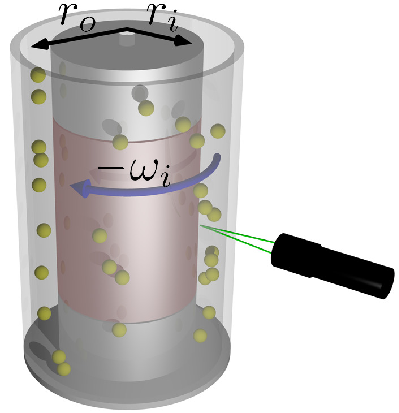
\includegraphics[height=5.5cm]{figure1.pdf}
\caption{
Schematic of the Taylor-Couette setup. Two concentric cylinders of radii
$r_{i,o}$ with a working fluid in between. Particles are not to scale. The
inner cylinder rotates with angular velocity $\omega_i$, while the outer
cylinder is kept at rest. We measure the torque on the middle section
(highlighted). The laser Doppler anemometry (LDA) probe is positioned at mid
height to measure the azimuthal velocity at mid gap.}
\label{fig:setup}
\end{figure}
The system is thermally controlled by cooling the top and bottom plates of the
setup. The temperature was kept at $T = \SI{20(1)}{\celsius}$ for all the
experiments, with a maximum spatial temperature difference of
$\SI{0.2}{\kelvin}$ within the setup, and we account for the density and
viscosity changes of water and glycerol \citep{Glycerine1963}.

Rigid polystyrene spherical particles (\textit{RGPballs S.r.l.}) were used in
the experiments, these particles have a density close to that of water
(940\,--\SI{1040}{\kilo\gram/\metre\cubed}). We chose particles with diameters
$d_p = 1.5$, 4.0, and $\SI{8.0}{\milli\metre}$. To our disposal are:
\SI{2.22}{\litre} of \SI{1.5}{\milli\metre} diameter particles,
\SI{2.22}{\litre} of \SI{4}{\milli\metre} diameter particles, and
\SI{6.66}{\litre} of \SI{8}{\milli\metre} diameter particles, resulting in
maximum volume fractions of \SI{2}{\percent}, \SI{2}{\percent}, and
\SI{6}{\percent}, respectively. The particles are found to be nearly
mono-disperse (\SI{99.9}{\percent} of the particles are within \SI{\pm
0.1}{\milli\metre} of their target diameter). Due to the fabrication process,
small air bubbles are sometimes entrapped within the particles. This results
in a slight heterogeneous density distribution of the particles. After
measuring the density distribution for each diameter, we calculated the
average for all batches, which is $\rho_p = \SI{1036 \pm
5}{\kilo\gram/\metre\cubed}$. By adding glycerol to water we match this value
in order to have neutrally buoyant particles.

Using a laser Doppler anemometry (LDA) system (BSA F80, Dantec Dynamics) we
captured the azimuthal velocity at mid-height and mid-gap of the system (see
\reff{fig:setup}) and we performed a radial scan at mid-height.
The flow was seeded with \SI{5}{\micro\metre} diameter polyamide particles
(PSP-5, Dantec Dynamics). Because of the curved surface of the outer cylinder
(OC), the beams of the LDA get refracted in a non-trivial manner, which was
corrected for using a ray-tracing technique \citep{Huisman2012}. 

Obviously, LDA measurements in a multi-phase flow are more difficult to set up
than for single phase flows, as the method relies on the reflection of
light from tiny tracer particles passing through a measurement volume
($\SI{0.07}{\milli\metre} \times \SI{0.07}{\milli\metre} \times
\SI{0.3}{\milli\metre}$).  Once we add a second type of relatively large
particles to the flow, this will affect the LDA measurements, mostly by
blocking the optical path, resulting in lower acquisition rates. These large
particles will also move through the measurement volume, but as these
particles are at least 300 times larger than the tracers and thus much larger
than the fringe pattern (fringe spacing $d_f=\SI{3.4}{\micro\metre}$), the
reflected light is substantially different from a \emph{regular} Doppler burst
and does not result in a measured value. The minimal signal-to-noise ratio for
accepting a Doppler burst was set to 4. As a post-processing step the
velocities were corrected for the velocity bias by using the transit time of
the tracer particle.
\newpage
\section{Results}\label{sec:sphereresults}
\subsection{Effect of particle size}\label{subsec:sizeEffect}
First we study the effect of changing the particle diameter on the torque of
the system. In these experiments, we kept the particle volume fraction fixed
at \SI{2}{\percent} and the density of the working fluid, $\rho_f$, at
\SI{1036}{\kilogram/\metre \cubed}, for which the particles are neutrally
buoyant. The results of these measurements are presented as
$\Nus_\omega(\Tay)$ in \reff{fig:TaNuwSize}. Our curves are practically
overlapping, suggesting that the difference in drag between the different
particle sizes is only marginal. We compare these with the bubbly drag
reduction data at similar conditions (hollow symbols) 
\citep{Verschoof2016,vanGils2013,vandenBerg2005}. At low $\Tay$ the symbols
overlap with our data. However, at larger $\Tay$, the bubbly flow data shows
much lower torque (drag) than the particle-laden cases. As we are in the
ultimate regime of turbulence where $\Nus_\omega$ effectively scales as
$\Nus_\omega \propto \Tay^{0.4}$~\citep{Huisman2012,Ostilla-Monico2013}, we
compensate the data with $\Tay^{0.40}$ in \reff{fig:TaNuwTaSize} to
emphasize the differences between the datasets. For the single phase
case, this yields a clear plateau. For the particle-laden cases, the lowest
drag corresponds to the smallest particle size. The reduction is however quite
small ($<\SI{3}{\percent}$). The compensated plots also reveal a sudden
increase in drag at a critical Taylor number $\Tay^* =\num{0.8e12}$. The jump
is more distinct for the smaller particles, and might suggest a reorganisation
of the flow \citep{Huisman2014}. Beyond $\Tay^*$, the drag reduction is
negligible for the larger particles (\SI{4}{\milli \metre} and \SI{8}{\milli
\metre} spheres). However, for the \SI{1.5}{\milli\metre} particles, the drag
reduction seems to increase, and was found to be very repeatable in
experiments. Interestingly, the size of these particles is comparable to that
of the air bubbles \citep{vanGils2013}.  This might suggest that for smaller
size particles at larger $\Tay$, one could expect drag reduction. At the
increased viscosity of the suspension, a maximum $\Tay \approx 3 \times
10^{12}$ could be reached in our experiments.   We have performed an
uncertainty analysis by repeating the measurements for the single phase, and
for the cases with \SI{8}{\milli\metre} and \SI{1.5}{\milli\metre} particles
multiple times and calculating the maximum deviation from the ensemble
average.  The left error bar indicates the maximum deviation for all
measurements combined and is $\approx \SI{1}{\percent}$.  For $\Tay \geq
\num{2e12}$, we see an increase in uncertainty of \SI{1.7}{\percent} (shown by
the right error bar in \reff{fig:TaNuwTaSize}), which is only caused by
the \SI{1.5}{\milli\metre} particles. These tiny particles can accumulate in
the \SI{2}{\milli\metre} gap between the cylinder segments and thereby
increase the uncertainty. Above $\Tay \geq \num{2e12}$, both, the
\SI{8}{\milli\metre} and \SI{4}{\milli\metre} particles, show a maximum
deviation below 0.25\%.\\
%
\begin{figure}
\centering%
\subfloat{%
    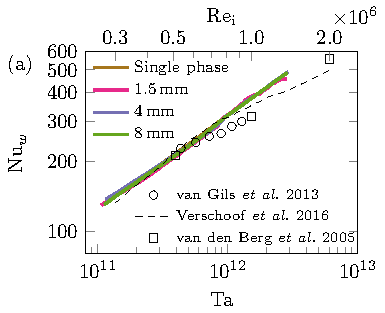
\includegraphics{figure2a.pdf}%
  \label{fig:TaNuwSize}
}%
\subfloat{%
    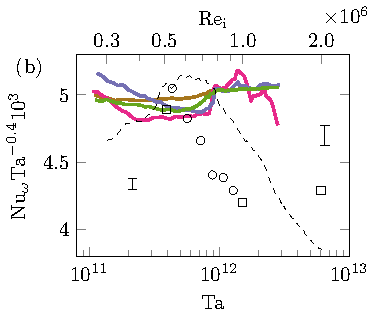
\includegraphics{figure2b.pdf}
  \label{fig:TaNuwTaSize}
}%
\caption{%
(a) $\Nus_\omega (\Tay)$ for \SI{2}{\percent} particle volume fraction with
particle diameters of \SI{1.5}{\milli\metre}, \SI{4.0}{\milli\metre}, and
\SI{8.0}{\milli\metre}, and for comparison the single phase case. Data from
comparable bubbly drag reduction studies are plotted using black markers. (b)
Same data, but now as compensated plot $\Nus_\omega / \Tay^{0.40}$ as function
of $\Tay$.   The error bar indicates the maximum deviation for repeated
measurements from all measurements combined (coloured curves) which is less
than \SI{1}{\percent}. At $\Tay \geq \num{2e12}$, the \SI{1.5}{\milli\metre}
particles show an increased uncertainty of \SI{1.7}{\percent}, which is
indicated by the right error bar.}
\label{fig:dragReductionSize}
\end{figure}
%
\indent Below $\Tay^*$, the drag reduction due to spherical particles appears to be
similar to bubbly drag reduction~\citep{vanGils2013}. However, in the lower
$\Tay$ regime, the bubble distribution was highly non-uniform due to buoyancy
of the bubbles~\citep{vandenBerg2005,vanGils2013,Verschoof2016}. Therefore,
the volume fractions reported were only the global values, and the torque
measurements were for the mid-sections of their setups. What is evident from
the above comparisons is that in the high $\Tay$ regime, air bubbles
drastically reduce the drag, reaching far beyond the drag modification by
rigid spheres.
\newpage
\subsection{Effect of particle volume fraction}\label{subsec:volumeFraction}
The next step is to investigate the effect of the particle volume fraction on
the torque. For the \SI{8}{\milli\metre} particles, we have the ability to
increase the particle volume fraction up to \SI{6}{\percent}. This was done in
steps of \SI{2}{\percent}, and the results are plotted in compensated form in
\reff{fig:TaNuwTaVF}. The normalised torque increases with the volume
fraction of particles. The \SI{6}{\percent} case shows the largest drag.
\refF{fig:TadrVF} shows the same data in terms of drag reduction as
function of $\Tay$. A \SI{2}{\percent} volume fraction of particles gives the
highest drag reduction. With increasing $\alpha$ the drag reduction decreases.
These measurements are in contrast with the findings for bubbly drag
reduction~\citep{vanGils2013}, for which the net drag decreases with
increasing gas volume fraction.
of drag in a particle-laden flow is the larger apparent viscosity.  If we
would calculate the apparent viscosity for our case with the Einstein relation
(\refe{eq:einstein}) for $\alpha=\SI{6}{\percent}$, the drag increase
would be \SI{15}{\percent}, as compared to the pure working fluid.  Including
this effect in our drag reduction calculation would result in reductions of
the same order.  However, when comparing the drag with or without particles,
the \emph{net} drag reduction is practically zero. This result is different
from the work a in turbulent channel flow where they found
that the drag increased more than the increase of the viscosity\citep{Picano2015}.

\begin{figure}
\centering%
\subfloat{%
    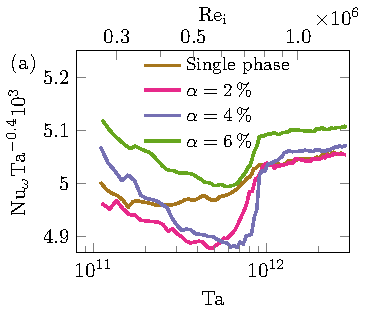
\includegraphics{figure3a.pdf}%
  \label{fig:TaNuwTaVF}
}%
\subfloat{%
    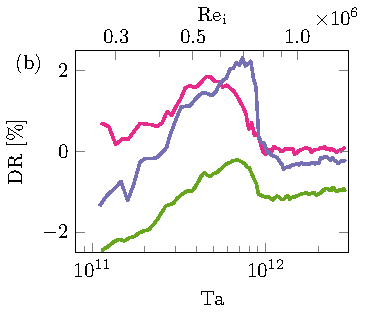
\includegraphics{figure3b.pdf}
  \label{fig:TadrVF}
}%
\caption{%
(a) $\Nus_\omega (\Tay)$, compensated by $\Tay^{0.4}$, for
\SI{8}{\milli\metre} particles with various particle volume fractions and for
comparison the single phase case.  (b) Drag reduction, defined as
$\text{DR} = \left(1 - \Nus_\omega(\alpha) / \Nus_\omega(\alpha=0) \right)$,
plotted against $\Tay$.
}
\label{fig:dragReductionVF}
\end{figure}

For a better comparison with bubbly drag reduction, we plot the drag reduction
as a function of (gas or particle) volume fraction $\alpha$; see 
\reff{fig:alphaDrAll}. Different studies are shown using different symbols, and
$\rey$ is indicated by colours. None of the datasets were compensated for the
changes in effective viscosity.   DR is defined in slightly differently
way in each study: van~den~Berg \citep{vandenBerg2005} makes use of the friction coefficient
$\left(1 - c_f(\alpha) /c_f(0) \right)$; van~Gils \citep{vanGils2013} uses the
dimensionless torque $G=\tau / (2 \pi L_{mid} \rho \nu^2)$, $\left(1 -
G(\alpha) / G(0) \right)$; and Verschoof \citep{Verschoof2016} uses the plain torque
value $\left(1 - \tau(\alpha) /\tau(0) \right)$. While the rigid particles
only showed marginal drag reduction, some studies using bubbles achieve
dramatic reduction of up to \SI{30}{\percent} and beyond. 
\refF{fig:alphaDrZoom} shows a zoomed in view of the bottom part of the plot
with the rigid sphere data. The triangles denote the data from
Verschoof \citep{Verschoof2016}, corresponding to small bubbles in the Taylor-Couette
system. The rigid particles and the small bubbles show a similar drag
response. What is remarkable is that this occurs despite the huge difference
in size. The estimated diameter of the bubbles in Verschoof \citep{Verschoof2016} is
\SI{0.1}{\milli \metre}, while the rigid spheres are about two orders in
magnitude larger. This provides key evidence that the particle size alone is
not enough to cause drag reduction, also the density ratio of the
particle and the carrier fluid is of importance.

\begin{figure}
\centering%
\subfloat{%
    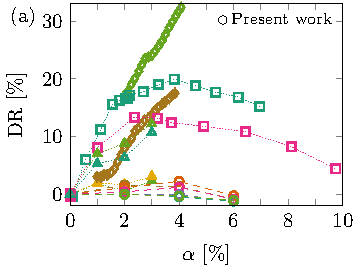
\includegraphics{figure4a.pdf}%
  \label{fig:alphaDrAll}
}%
\subfloat{%
    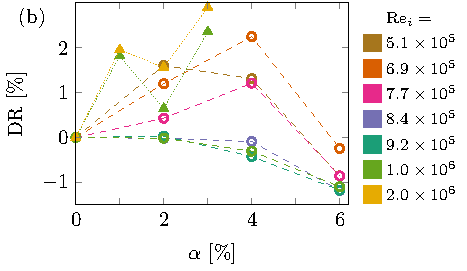
\includegraphics{figure4b.pdf}%
  \label{fig:alphaDrZoom}
}%
\caption[]{(a) Drag reduction as function of particle volume fraction from
    \marksymbol{o}{black}\,: $d_p=\SI{8}{\milli\metre}$ particles from
    present work compared to similar gas volume fractions from
    \marksymbol{square}{black}\,: van~den~Berg\citep{vandenBerg2005},
    \marksymbol{diamond}{black}\,: van~Gils\citep{vanGils2013}, and
    \marksymbol{triangle}{black}\,: Verschoof\citep{Verschoof2016}. Symbols indicate the
    different studies while colours differentiate between the Reynolds
    numbers. The current work has DR defined as $\left(1 -
        \Nus_\omega(\alpha) / \Nus_\omega(\alpha=0) \right)$; the other
        studies use dimensionless torque $G$ \citep{vanGils2013}, friction
        coefficient $c_f$ \citep{vandenBerg2005}, or plain torque $\tau$
        \citep{Verschoof2016} to define DR. (b) Zoom of the bottom part of
    (a) where the data from the present work is compared to bubbly drag
reduction data using \SI{6}{ppm} of surfactant \citep{Verschoof2016}}
\label{fig:dragReductionAlpha}
\end{figure}

\subsection{Effect of marginal changes in particle density ratio}
With the effects of particle size and volume fraction revealed, we next
address the sensitivity of the drag to marginal variations in particle
density. A change in the particle density ratio brings about a change in the
buoyancy and  centrifugal forces on the particle, both of which can affect the
particle distribution within the flow. We tune the particle to fluid density
ratio $\phi \equiv \rho_p/\rho_f$ by changing the volume fraction of glycerol
in the fluid, such that the particles are marginally buoyant ($\phi = 0.94,
0.97$), neutrally buoyant ($\phi=1.00$) and marginally heavy ($\phi=1.04$)
particles. In \reff{fig:TaNuwTaDen} we show the compensated
$\Nus_\omega$ as function of $\Tay$ for various $\phi$. $\alpha$ was fixed to
\SI{6}{\percent} and only \SI{8}{\milli\metre} particles were used. The darker
shades of colour correspond to the single phase cases, while lighter shades
correspond to particle-laden cases. In general, the single phase drag is
larger as compared to the particle-laden cases. However, there is no striking
difference between the different $\phi$.  In \reff{fig:TaDrDen}, we
present the drag reduction for particle-laden cases at different density
ratios. On average we see for all cases drag modification of approximately
$\pm$ \SI{2}{\percent}. We can also identify a small trend in the lower $\Tay$
region: the two larger $\phi$ (heavy and neutrally buoyant particles) tend to
have a drag increase, while the smaller $\phi$ cases (both light particles)
have a tendency for drag reduction. Nevertheless, the absolute difference in
DR between the cases is within 4\%. The above results provide clear evidence
that minor density mismatches do not have a serious influence on the global
drag of the system.  To investigate for strong buoyancy effects,
additional measurements were done using \SI{2}{\milli\metre} expanded
polystyrene particles ($\phi=0.02$).  However, due to the particles
accumulating between the inner cylinder segments leading to additional
mechanical friction, these measurements were inconclusive.

\begin{figure}
\centering
\subfloat{
    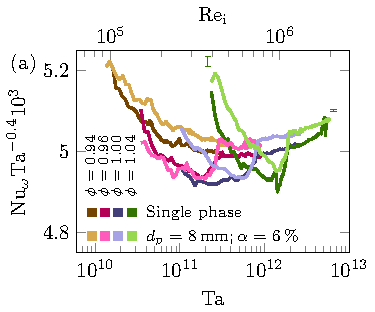
\includegraphics{figure5a.pdf}
  \label{fig:TaNuwTaDen}
}
\subfloat{
    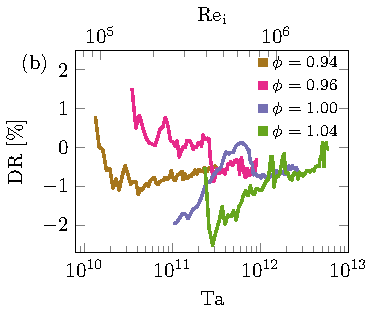
\includegraphics{figure5b.pdf}
  \label{fig:TaDrDen}
}
\caption{
(a) $\Tay$ as function of $\Nus_\omega$ compensated by $\Tay^{0.4}$ for
various density ratios $\phi=\rho_p/\rho_f$ indicated by the corresponding
colour. The darker shades indicate the single phase cases while the
lighter shades show the cases using \SI{6}{\percent} particle volume
fraction of \SI{8}{\milli\metre} diameter particles. Due to the increase
in viscosity the maximum attainable $\Tay$ is lower for larger density
ratios. The uncertainty is again estimated using the maximum
deviation from the average for multiple runs and here only shown for
the green curves. This value is slightly below \SI{1}{\percent} at
lower $\Tay$ and decreases with increasing $\Tay$ to values below
\SI{0.25}{\percent}. This trend is seen for all $\phi$.  (b) 
Drag reduction, calculated from the data of figure 5a, plotted against
$\Tay$. The drag reduction is defined as $\text{DR} = \left(1 -
\Nus_\omega(\alpha=6\%) / \Nus_\omega(\alpha=0) \right)$.
}
\label{fig:dragReductionDen}
\end{figure}
\newpage
\subsection{Flow statistics using particles} 
In the above sections, we presented the effects of changing particle size,
volume fraction, and density on the global drag of the system. Next we look
into local flow
properties using LDA while the particles are present.  First, we collected a
total of \num{1e6} data points of azimuthal velocity at mid-height and
mid-gap.  These were captured over a period of approximately $\num{3e4}$
cylinder rotations. From this data we calculate the probability density
function (PDF) of $\text{u}_\theta$ normalised by $u_i$ for various $\alpha$,
shown in \reff{fig:U_w_pdf}. The particle size was fixed to
\SI{8}{\milli\metre} and the Reynolds number was set to $\num{1e6}$. From this
figure we see a large increase in turbulent fluctuations, resulting in very
wide tails. While the difference between \SI{2}{\percent}, \SI{4}{\percent},
and \SI{6}{\percent} is not large, we can identify an increase in fluctuations
with increasing $\alpha$. These increased fluctuations can be explained by the
additional wakes produced by the particles \citep{Poelma2007,Almeras2017}. The
increase in fluctuations can also be visualized using the standard deviation
of $\sigma(u_\theta) = \left< \text{u}_\theta'^2 \right>^{1/2}$ normalised by
the standard deviation of the single phase case---see 
\reff{fig:alpha_u_rms_u0}. In this figure, $\sigma(u_\theta)$ is shown for
three different $\rey$, again for \SI{8}{\milli\metre} particles. In general,
we see a monotonically increasing trend with $\alpha$, and it seems to
approach an asymptotic value. One can speculate that there has to be an upper
limit for fluctuations which originate from wakes of the particles. For large
$\alpha$ the wakes from particles will interact with each other and with the
carried flow.

\begin{figure}
\centering%
\subfloat{%
    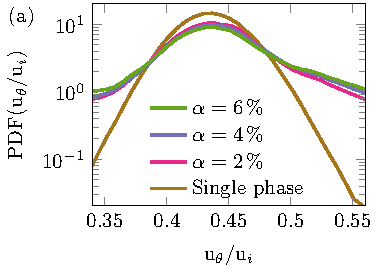
\includegraphics{figure6a.pdf}%
  \label{fig:U_w_pdf}
}%
\subfloat{%
    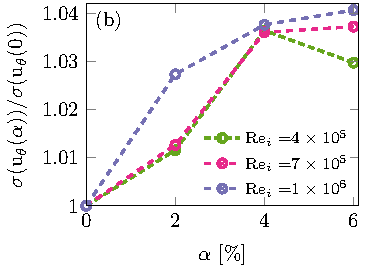
\includegraphics{figure6b.pdf}%
  \label{fig:alpha_u_rms_u0}
}%
\caption{%
(a) PDF of $\text{u}_\theta / \text{u}_i$ for various $\alpha$ and the
single phase case. The particle size was fixed to \SI{8}{\milli\metre}
and $\rey_i=\num{1e6}$ for all cases. (b) Standard deviation of the
azimuthal velocity normalized by the standard deviation of the single phase
case for three different $\rey$ for a fixed particle size of
\SI{8}{\milli\metre}.} \label{fig:ldaresults}
\end{figure}

Measurements using \SI{4}{\milli\metre} particles yielded qualitatively
similar results. It is known that in particle-laden gaseous pipe flows, large
particles can increase the turbulent fluctuations, while small particles
result in turbulence attenuation \citep{Tsuji1984,Gore1989,Vreman2015}. The
LDA measurements were not possible with the smallest particles
(\SI{1.5}{\milli\metre}), as the large amount of particles in the flow blocked
the optical paths of the laser beams.

We are confident that for these bi-disperse particle-laden LDA measurements,
the large particles do not have an influence on the measurements as these
\emph{millimetric}-sized particles are much larger than the fringe spacing
($d_f = \SI{3.4}{\micro\metre}$) and do not show a Doppler burst.  However,
during the measurements the particles get damaged and small bits of material
are fragmented off the particles. We estimate the size of these particles
slightly larger than the tracer particles and these can have an influence on
the LDA measurements as they do not act as tracers.

How the average azimuthal velocity changes with particle radius is shown in
\reff{fig:ldaradial}.  We measured a total of $\num{3e4}$ data points
during approximately 900 cylinder rotations. Again, the data were corrected
for velocity bias by using the transit time as a weighing factor. 
\refF{fig:U_theta_radius_size} shows the effect of particle size for
$\alpha=\SI{2}{\percent}$, and \reff{fig:U_theta_radius_vol} shows the
effect of particle volume fraction for \SI{8}{\milli\metre} particles. Both
figures additionally show the high-precision single phase data from another
study \citep{Huisman2013} for which our single phase measurements are practically
overlapping. Since LDA measurements close to the inner cylinder are difficult,
due to the reflecting inner cylinder surface, we limited our radial extent to
$\tilde{r}=(r - r_i) / (r_o - r_i)=[0.2,1]$. We found that the penetration
depth of our LDA measurements is the smallest for experiments with the
smallest particles and the largest $\alpha$. All differences with the single
phase case are only marginal and we can conclude that the average mean
velocity is not much affected by the particles in the flow, at least for
$\tilde{r} \geq 0.2$.

\begin{figure}
\centering%
\subfloat{%
    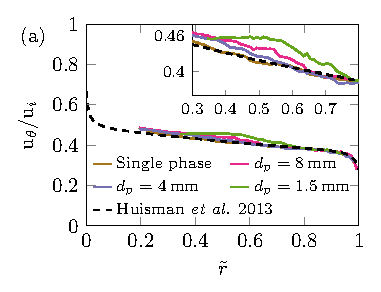
\includegraphics{figure7a.pdf}%
  \label{fig:U_theta_radius_size}
}%
\subfloat{%
    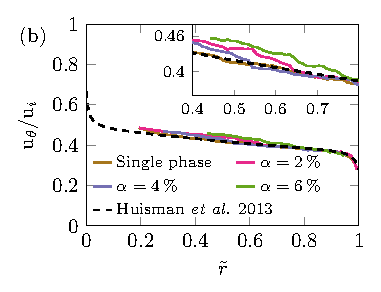
\includegraphics{figure7b.pdf}%
  \label{fig:U_theta_radius_vol}
}%
\caption{%
$\text{u}_\theta$ normalised by the velocity of the inner cylinder wall
$\text{u}_i$ as function of the normalised radius for various $d_p$ while
$\alpha=\SI{2}{\percent}$ (a) and various $\alpha$ while
$d_p=\SI{8}{\milli\metre}$ (b). In all cases $\rey_i$ is fixed to $\num{1e6}$.
For comparison, the single phase case using water at $\rey_i=\num{1e6}$ from
Huisman~\citep{Huisman2013} is also plotted in dashed black in both plots. Both figures
have an inset showing an enlargement of the centre area from the same
figure.} \label{fig:ldaradial}
\end{figure}

\begin{figure}
\centering%
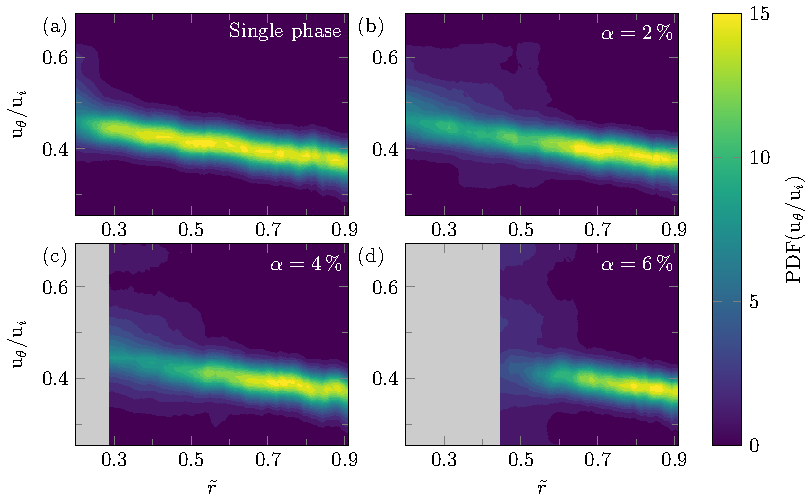
\includegraphics{figure8.pdf}%
\caption{%
\label{fig:heatmap}
PDF of the normalised azimuthal velocity as a function of normalised radial
position for various $\alpha$ for the case of \SI{8}{\milli\metre} particles
and the single phase case while keeping $\rey$ at $\num{1e6}$. With increasing
$\alpha$ the maximum penetration depth decreases. The grey areas indicate
radial positions for which no data is available.
}
\end{figure}

To get an idea of the fluctuations we can use the previous data to construct a
two-dimensional PDF of the azimuthal velocity as function of radius. These are
shown for $\rey = \num{1e6}$ using \SI{8}{\milli\metre} particles at various
$\alpha$ and the single phase case in \reff{fig:heatmap}.  First thing
to notice is again that the penetration depth is decreasing with increasing
$\alpha$.  The single phase case shows a narrow banded PDF. When $\alpha$ is
increased, for the lower values of $\tilde{r}$ the PDF is much wider.  While
it makes sense that an increase in $\alpha$ increases the fluctuations due to
the increased number of wakes of particles, this is expected everywhere in the
flow, not only closer to the inner cylinder.  It is possible that the
particles have a preferred concentration closer to the inner cylinder.  We
have tried to measure the local concentration of particles as function of
radius but failed due to limited optical accessibility.  Therefore, we can
only speculate under what circumstances there would be an inhomogeneous
particle distribution which would lead to the visible increase in
fluctuations.  The first possibility is a mismatch in density between the
particle and the fluid, which would result in light particles ($\phi < 1$) to
accumulate closer to the inner cylinder.  Another possibility is that due to
the rotation of the particle, an effective lift force arises, leading to a
different particle distribution in the flow. While this is quite plausible,
this is difficult to validate as we would need to capture the rotation.  The
fragments of plastic that are sheared off the particles can also have a bias
to the LDA measurement. While we estimate them to be larger than the tracers,
they might still be small enough to produce a signal and they might not follow
the flow faithfully.

\section{Conclusions and outlook}\label{sec:conclusions_and_outlook}
We have conducted an experimental study on the drag response of a highly
turbulent Taylor-Couette flow containing rigid neutrally buoyant spherical
particles. We have found that, unlike the case of bubbles used in prior
works~\citep{vanGils2013,Verschoof2016}, rigid particles barely reduce (or
increase) the drag on the system, even for cases where their size was
comparable to that of bubbles used in other studies.
There was no significant size effect. Even for very large particles, which can
attenuate turbulent fluctuations and generate wakes, there was no distinct
difference with the single phase flow.
We also varied the volume fraction of the particles in the range 0\%--6\%. The
particle volume fraction has no greater effect on the system drag than what is
expected due to changes in the apparent viscosity of the suspension. Further,
we tested the sensitivity of our drag measurements to marginal variations in
particle to fluid density ratio $\phi$. A trend was noticeable, towards drag
reduction when $\phi$ was reduced from 1.00 to 0.94. This suggests that a low
density of the particle could be a necessary ingredient for drag reduction.
Finally, we have also probed the local flow at the mid height and mid gap of
the system using LDA. With the addition of particles, the liquid velocity
fluctuations are enhanced, with wider tails of the distributions. A finite
relative velocity between the particle and the flow around it can cause this
increase in velocity fluctuations~\citep{Mathai2015}, as seen for bubbly flows
(pseudo-turbulence), and in situations of sedimenting particles in quiescent
or turbulent environments~\citep{Gore1989}.  In the present situation, the
relative velocity between the particle and the flow is expected, owing to the
inertia of the finite-sized particles we used.
There is only a marginal deviation from the single phase case in the average
azimuthal velocity over the radial positions measured using any size or
concentration of particles measured. From the two-dimensional PDFs, we see
that closer to the inner cylinder, using smaller $d_p$ or larger $\alpha$, the
PDF gets wider. This can be due to a preferential concentration of the
particles or a slight density mismatch.

\textcolor{black}{Our study is a step towards a better understanding of the
mechanisms of bubbly drag reduction. Bubbles are deformable, and they have
a tendency to migrate towards the walls, either due to lift
force~\citep{Dabiri2013}, or due to the centripetal
effects~\citep{vanGils2013}. When compared to the drag reducing bubbles 
\citep{vanGils2013,Verschoof2016}, our particles do not deform, and they do
not experience centripetal effects as they are density matched.  At
least one of these differences must therefore be crucial for the observed,
bubbly drag reduction in those experiments.
In a future investigation, we will conduct more experiments using very light
spherical particles that experience similar centripetal forces as the bubbles
in van~Gils~\citep{vanGils2013}, but are non-deformable.} These particle need to be
larger than the size of the gap between the inner cylinder segments and very
rigid, or the setup needs to be modified to close the gap between the IC
segments.  Such experiments can then disentangle the role of particle density
on drag reduction from that of the particle shape.

\graphicspath{{fig/}}



% Chapters
%%%%%%%%%%%%%%%%%%%%%%%%%%%
%%% Chapter definitions %%%
%%%%%%%%%%%%%%%%%%%%%%%%%%%
% Chapter title
\renewcommand{\mychaptertitle}{%
Finite-sized rigid spheres in turbulent Taylor-Couette flow: %
Effect on the overall drag%
}
% Chapter short title
\renewcommand{\mychaptershorttitle}{%
Finite-sized rigid spheres in turbulent Taylor-Couette flow%
}
% Chapter authors
\renewcommand{\mychapterauthors}{%
\textbf{Dennis~Bakhuis},
Ruben~A.~Verschoof,
Varghese~Mathai,
Sander~G.~Huisman,
Detlef~Lohse,
and
Chao~Sun
\textit{Finite-sized rigid spheres in turbulent Taylor-Couette flow:
Effect on the overall drag},
J. Fluid Mech. \textbf{850}, 246--261 (2018).
}
% Chapter abstract
\renewcommand{\mychapterabstract}{%
We report on the modification of drag by neutrally buoyant spherical
finite-sized particles in highly turbulent Taylor-Couette (TC) flow.  These
particles are used to disentangle the effects of size, deformability, and
volume fraction on the drag, and are contrasted with the drag in bubbly TC
flow.  From global torque measurements we find that rigid spheres hardly
decrease or increase the torque needed to drive the system.   The size of the
particles under investigation have a marginal effect on the drag, with smaller
diameter particles showing only slightly lower drag.  Increasing the particle
volume fraction shows a net drag increase, however this increase is much
smaller than can be explained by the increase in apparent viscosity due to the
particles.  The increase in drag for increasing particle volume fraction is
corroborated by performing laser Doppler anemometry where we find that the
turbulent velocity fluctuations also increase with increasing volume fraction.
In contrast with rigid spheres, for bubbles the effective drag reduction also
increases with increasing Reynolds number. Bubbles are also much more
effective in reducing the overall drag. 
}
\renewcommand{\mychaptermark}{Neutrally buoyant spheres}
\renewcommand{\mychapterlabel}{chap:spheres}
\renewcommand{\mychaptericon}{fig/swchapter1.png}
%%%%%%%%%%%%%%%%%%%%%%%%%%%%%
%%% Create Chapter Header %%%
%%%%%%%%%%%%%%%%%%%%%%%%%%%%%
%%%%%%%%%%%%%%%%%%%%%%
%%% Chapter header %%%
%%%%%%%%%%%%%%%%%%%%%%
\globalcolor{ChapterText}
\chapter[\mychaptershorttitle]{%
    \mychaptertitle%
    \ifdefined\starwarsfootnotes
        \textsuperscript{%
            \hspace{-1mm}%
            \includegraphics[height=\swsymsize]{\mychaptericon}%
        }%
        \blfootnote{%
            \textcolor{footnotetextcolor}{%
                \textsf{%
                    \vspace{0.5mm}\hspace{-1mm}%
                    \includegraphics[height=\swfnsymsize]{\mychaptericon}%
                    \hspace{0.5mm}%
                    Based on: \mychapterauthors%
                }
            }
        }
    \else
        \footnote{\textsf{%
             Based on: \mychapterauthors%
        }}%
    \fi
}
\pagecolor{ChapterBackground}
\afterpage{\pagecolor{White}\globalcolor{Black}} 
\label{\mychapterlabel}
\chaptermark{\mychaptermark}
\noindent\rule{\textwidth}{0.4pt}%
\vspace{0.2cm}
\noindent\textsf{\mychapterabstract}
\clearpage

%%%%%%%%%%%%%%%%%%%%%%%%
%%%% end title page %%%%
%%%%%%%%%%%%%%%%%%%%%%%%
\graphicspath{{ChapterOne/fig/}}
\section{Introduction}
Flows in nature and industry are generally turbulent, and often these flows
carry bubbles, drops, or particles of various shapes, sizes, and densities.
Examples include sediment-laden rivers, gas-liquid reactors, volcanic
eruptions, plankton in the oceans, pollutants in the atmosphere, and air
bubbles in the ocean mixing layer~\citep{Toschi2009}.  Particle-laden flows
may be characterized in terms of particle density $\rho_p$, particle diameter
$d_p$, volume fraction $\alpha$, and Reynolds number Re of the flow. When
$d_p$ is small (compared to the dissipative length scale $\eta_K$) and
$\alpha$ low ($< 10^{-3}$), the system may be modelled using a point particle
approximation with two-way
coupling~\citep{Elghobashi1994,Mazzitelli2003,Mathai2016}.  With recent
advances in computing, fully resolved simulations of particle-laden flows have
also become feasible.  Uhlmann conducted one of the first numerical
simulations of finite-sized rigid spheres in a vertical particle-laden channel
flow \citep{Uhlmann2008}.  They observed a modification of the mean velocity
profile and turbulence modulation due to the presence of particles. A number
of studies followed, which employed immersed
boundary~\citep{Peskin2002,Cisse2013}, Physalis~\citep{Naso2010, Wang2017b},
and front-tracking methods~\citep{Unverdi1992,Roghair2011,Tagawa2013} to treat
rigid particles and deformable bubbles, respectively, in channel and pipe flow
geometries~\citep{Pan1996,Lu2005,Uhlmann2008,Dabiri2013,Kidanemariam2013,Lashgari2014,Picano2015,Costa2016}. 
Flows with dispersed particles, drops, and bubbles can, under the right
conditions, reduce skin friction and result in significant energetic (and
therefore financial) savings. In industrial settings this is already achieved
using polymeric additives which disrupt the self-sustaining cycle of wall
turbulence and dampen the quasi-streamwise vortices
\citep{White2008,Procaccia2008}. Polymeric additives are impractical for
maritime applications, and therefore gas bubbles are used with varying success
rates \citep{Ceccio2010,Murai2014}. Local measurements in bubbly flows are
non-trivial and the key parameters and their optimum values are still unknown.
For example, it is impossible to fix the bubble size in experiments and
therefore to isolate the effect of bubble size. Various studies hinted that
drag reduction can also be achieved using spherical particles
\citep{Zhao2010}, also by using very large particles in a turbulent von
K\'arm\'an flow \citep{Cisse2015}. In this latter study a tremendous decrease
in turbulent kinetic energy (TKE) was observed. A similar, but less intense,
decrease in TKE was also seen using a very low particle volume
fraction\citep{Bellani2012b}. By using solid particles it is possible to
isolate the size effect on drag reduction and even though rigid particles are
fundamentally different from bubbles, this can give additional insight into
the mechanism of bubbly drag reduction.  The particle dynamics are highly
influenced by the diameter of the particle\citep{Machicoane2016}. This might
or might not have a direct influence on the global drag of the system and has
never been studied.
%
Whether and when solid particles increase or decrease the drag in a flow is
yet not fully understood and two lines of thought exist. On one side, it is
hypothesized that solid particles {\it decrease} the overall drag as they damp
turbulent fluctuations \citep{Zhao2010,Poelma2007}. On the other side, one
could expect that solid particles {\it increase} drag as they shed vortices,
which must be dissipated. In addition, they also increase the apparent
viscosity. A common way to quantify this is the so called `Einstein
relation'~\citep{Einstein1906}
\begin{equation} \nu_\alpha = \nu\left(1 +
\frac{5}{2}\alpha \right), \label{eq:einstein} \end{equation} where $\nu$ is
the viscosity of the continuous phase. This compensation is valid for the
small $\alpha$ values used in this \docname \citep{Stickel2005}. Direct
measurements of drag in flows with solid particles are scarce, and the debate
on under what condition they either enhance or decrease the friction has not
yet been settled. Particles and bubbles may show collective effects
(clustering) and experiments have revealed that this has significant influence
on the flow properties~\citep{Liu1993, Kulick1994, Muste1997, So2002,
Fujiwara2004, vandenBerg2005, vandenBerg2007, Shawkat2008, Calzavarini2008,
Colin2012, vanGils2013, Maryami2014, Mathai2015,
Almeras2017,Mathai2018}. In general, the Stokes number is used to
predict this clustering behaviour, but for neutrally buoyant particles this is
found to be insufficient \citep{Bragg2015,Fiabane2012}. In addition, the
position of the particles (or the particles clusters) is likely to have a
large influence on the skin friction.  It was shown in DNS at low Reynolds
numbers, that the particle distribution is mainly
governed by the bulk Reynolds number\citep{Kazerooni2017}.

In order to study the effects of particles on turbulence it is convenient to
use a closed setup where one can relate global and local quantities directly
through rigorous mathematical relations. In this \docname the Taylor-Couette
(TC) geometry~\citep{Grossmann2016}---the flow between two concentric rotating
cylinders---is employed as this is a closed setup with global balances. The
driving of the Taylor-Couette geometry can be described using the Reynolds
number based on the inner cylinder (IC): $\rey_i = u_i d / \nu$, where $u_i =
\omega_i r_i$ is the azimuthal velocity at the surface of the IC, $\omega_i$
the angular velocity of the IC, $d = r_o - r_i$ the gap between the cylinders,
$\nu$ the kinematic viscosity, and $r_i$($r_o$) the radius of the inner(outer)
cylinder. The geometry of Taylor-Couette flow is characterized by two
parameters: the radius ratio $\eta=r_i/r_o$ and the aspect ratio $\Gamma =
L/d$, where $L$ is the height of the cylinders. The response parameter of the
system is the torque, $\tau$, required to maintain constant rotation speed of
the inner cylinder. It was mathematically shown that in Taylor-Couette flow
the angular velocity flux defined as $J^\omega = r^3 \left(  \left
\langle u_r \omega \right \rangle_{A,t} - \nu \frac{\partial} {\partial r}
\left \langle \omega \right \rangle_{A,t} \right)$, where the subscript $A,t$
denotes averaging over a cylindrical surface and time,	is a radially
conserved quantity (Eckhardt, Grossmann, Lohse \citep{Eckhardt2007} (EGL)). One can, in analogy to
Rayleigh-B\'enard convection, normalize this flux and define a Nusselt number
based on the flux of the angular velocity:
\begin{equation}
  \Nus_\omega = \frac{J^\omega}{J^\omega_{\text{lam}}} = \frac{\tau}{2 \pi L \rho J^\omega_{\text{lam}}},
\end{equation}
where $J^\omega_{\text{lam}} = 2 \nu r^2_i r^2_o \left( \omega_i - \omega_o
\right)/\left( r^2_o - r^2_i \right)$ is the angular velocity flux for
laminar, purely azimuthal flow and $\omega_o$ is the angular velocity of the
outer cylinder. In this spirit the driving is expressed in terms of the Taylor
number:
\begin{equation}
  \Tay = \frac{1}{4} \sigma d^2 \left(r_i + r_o \right)^2 \left( \omega_i - \omega_o \right)^2 \nu^{-2}.
\end{equation}
Here $\sigma = \left( \left( 1 + \eta \right) / \left(2 \sqrt{\eta} \right)
\right)^4\;\approx\;1.057$ is a geometric parameter (``geometric Prandtl
number''), in analogy to the Prandtl number in Rayleigh-B\'enard convection.
In the presented work, where only the inner cylinder is rotated and the outer
cylinder is kept stationary, we can relate $\Tay$ to the Reynolds number of
the inner cylinder by
\begin{equation}
\rey_i = \frac{r_i \omega_i d}{\nu} = \frac{8\eta^2}{(1+\eta)^{3}} \sqrt{\Tay}.
\end{equation}
\noindent The scaling of the dimensionless angular velocity flux (torque) with
the Taylor (Reynolds) number has been analysed extensively, see e.g.
\citep{Lathrop1992,Lewis1999,Paoletti2011,vanGils2011,Ostilla-Monico2013} and
the review articles \citep{Fardin2014,Grossmann2016}, and the
different regimes are well understood. In the current Taylor number regime it
is known that $\Nus_\omega \propto \Tay^{0.4}$. Because this response is
well known, it can be exploited to study the influence of immersed bubbles and
particles
~\citep{vandenBerg2005,vandenBerg2007,vanGils2013,Maryami2014,Verschoof2016}
on the drag needed to sustain constant rotational velocity of the inner
cylinder. 

In this \docname we will use the TC geometry to study the effect of neutrally
buoyant rigid spherical particles on the drag. We study the effects of varying
the particle size $d_p$, the volume fraction $\alpha$, the density ratio
$\phi$, and the flow Reynolds number $\text{Re}$ on the global torque (drag)
of the Taylor-Couette flow. The drag reduction is expressed as $\text{DR} =
\left(1 - \Nus_\omega(\alpha) / \Nus_\omega(\alpha=0) \right)$ and as we are
interested in the net drag reduction, it is \emph{not} compensated for
increased viscosity effects using correction models, such as the Einstein
relation.

The \docname is organized as follows. \refSec{sec:experimentalSetup}
presents the experimental setup. In \refsec{sec:sphereresults} we discuss the
results. The findings are summarized and an outlook for future work is given
in the last section.

\section{Experimental setup}\label{sec:experimentalSetup}
The experiments were conducted in the Twente Turbulent Taylor-Couette
(T${}^3$C) facility \citep{vanGils2011}. A schematic of the setup is shown in
\reff{fig:setup}. In this setup, the flow is confined between two
concentric cylinders, which rotate independently. The top and bottom plates
are attached to the outer cylinder. The radius of the inner cylinder (IC) is
$r_i = \SI{0.200}{\metre}$ and the radius of the outer cylinder (OC) is $r_o =
\SI{0.2794}{\metre}$, resulting in a gap width of $d = r_o - r_i =
\SI{0.0794}{\metre}$ and a radius ratio of $\eta = r_i/r_o = 0.716$. The IC
has a total height of $L = \SI{0.927}{\metre}$ resulting in an aspect ratio of
$L / d = 11.7$. The IC is segmented axially in three parts. To minimize the
effect of the stationary end plates, the torque is measured only over the
middle section of the IC with height $L_{\text{mid}}/L = 0.58$, away from
the end plates. A hollow reaction torque sensor made by Honeywell is used to
measure the torque which has an error of roughly 1\% for the largest torques
we measured. Between the middle section and the top and bottom section of the
inner cylinder is a gap of 2mm.

The IC can be rotated up to $f_i = \omega_i/(2\pi) =
\SI{20}{\hertz}$. In these experiments only the IC is rotated and the OC is
kept at rest. The system holds a volume of $V = \SI{111}{\litre}$ of working
fluid, which is a solution of glycerol ($\rho =
\SI{1260}{\kilo\gram/\metre\cubed}$) and water. To tune the density of the
working fluid, the amount of glycerol was varied between \SI{0}{\percent} and
\SI{40}{\percent} resulting in particles being marginally heavy,
neutrally buoyant, or marginally light.
\begin{figure}
\centering
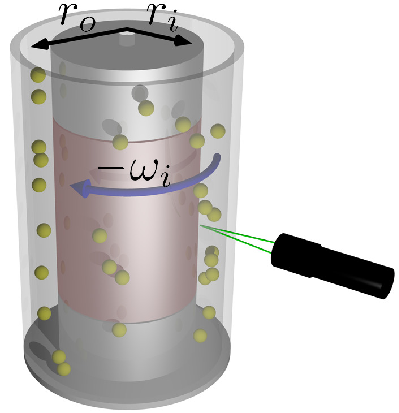
\includegraphics[height=5.5cm]{figure1.pdf}
\caption{
Schematic of the Taylor-Couette setup. Two concentric cylinders of radii
$r_{i,o}$ with a working fluid in between. Particles are not to scale. The
inner cylinder rotates with angular velocity $\omega_i$, while the outer
cylinder is kept at rest. We measure the torque on the middle section
(highlighted). The laser Doppler anemometry (LDA) probe is positioned at mid
height to measure the azimuthal velocity at mid gap.}
\label{fig:setup}
\end{figure}
The system is thermally controlled by cooling the top and bottom plates of the
setup. The temperature was kept at $T = \SI{20(1)}{\celsius}$ for all the
experiments, with a maximum spatial temperature difference of
$\SI{0.2}{\kelvin}$ within the setup, and we account for the density and
viscosity changes of water and glycerol \citep{Glycerine1963}.

Rigid polystyrene spherical particles (\textit{RGPballs S.r.l.}) were used in
the experiments, these particles have a density close to that of water
(940\,--\SI{1040}{\kilo\gram/\metre\cubed}). We chose particles with diameters
$d_p = 1.5$, 4.0, and $\SI{8.0}{\milli\metre}$. To our disposal are:
\SI{2.22}{\litre} of \SI{1.5}{\milli\metre} diameter particles,
\SI{2.22}{\litre} of \SI{4}{\milli\metre} diameter particles, and
\SI{6.66}{\litre} of \SI{8}{\milli\metre} diameter particles, resulting in
maximum volume fractions of \SI{2}{\percent}, \SI{2}{\percent}, and
\SI{6}{\percent}, respectively. The particles are found to be nearly
mono-disperse (\SI{99.9}{\percent} of the particles are within \SI{\pm
0.1}{\milli\metre} of their target diameter). Due to the fabrication process,
small air bubbles are sometimes entrapped within the particles. This results
in a slight heterogeneous density distribution of the particles. After
measuring the density distribution for each diameter, we calculated the
average for all batches, which is $\rho_p = \SI{1036 \pm
5}{\kilo\gram/\metre\cubed}$. By adding glycerol to water we match this value
in order to have neutrally buoyant particles.

Using a laser Doppler anemometry (LDA) system (BSA F80, Dantec Dynamics) we
captured the azimuthal velocity at mid-height and mid-gap of the system (see
\reff{fig:setup}) and we performed a radial scan at mid-height.
The flow was seeded with \SI{5}{\micro\metre} diameter polyamide particles
(PSP-5, Dantec Dynamics). Because of the curved surface of the outer cylinder
(OC), the beams of the LDA get refracted in a non-trivial manner, which was
corrected for using a ray-tracing technique \citep{Huisman2012}. 

Obviously, LDA measurements in a multi-phase flow are more difficult to set up
than for single phase flows, as the method relies on the reflection of
light from tiny tracer particles passing through a measurement volume
($\SI{0.07}{\milli\metre} \times \SI{0.07}{\milli\metre} \times
\SI{0.3}{\milli\metre}$).  Once we add a second type of relatively large
particles to the flow, this will affect the LDA measurements, mostly by
blocking the optical path, resulting in lower acquisition rates. These large
particles will also move through the measurement volume, but as these
particles are at least 300 times larger than the tracers and thus much larger
than the fringe pattern (fringe spacing $d_f=\SI{3.4}{\micro\metre}$), the
reflected light is substantially different from a \emph{regular} Doppler burst
and does not result in a measured value. The minimal signal-to-noise ratio for
accepting a Doppler burst was set to 4. As a post-processing step the
velocities were corrected for the velocity bias by using the transit time of
the tracer particle.
\newpage
\section{Results}\label{sec:sphereresults}
\subsection{Effect of particle size}\label{subsec:sizeEffect}
First we study the effect of changing the particle diameter on the torque of
the system. In these experiments, we kept the particle volume fraction fixed
at \SI{2}{\percent} and the density of the working fluid, $\rho_f$, at
\SI{1036}{\kilogram/\metre \cubed}, for which the particles are neutrally
buoyant. The results of these measurements are presented as
$\Nus_\omega(\Tay)$ in \reff{fig:TaNuwSize}. Our curves are practically
overlapping, suggesting that the difference in drag between the different
particle sizes is only marginal. We compare these with the bubbly drag
reduction data at similar conditions (hollow symbols) 
\citep{Verschoof2016,vanGils2013,vandenBerg2005}. At low $\Tay$ the symbols
overlap with our data. However, at larger $\Tay$, the bubbly flow data shows
much lower torque (drag) than the particle-laden cases. As we are in the
ultimate regime of turbulence where $\Nus_\omega$ effectively scales as
$\Nus_\omega \propto \Tay^{0.4}$~\citep{Huisman2012,Ostilla-Monico2013}, we
compensate the data with $\Tay^{0.40}$ in \reff{fig:TaNuwTaSize} to
emphasize the differences between the datasets. For the single phase
case, this yields a clear plateau. For the particle-laden cases, the lowest
drag corresponds to the smallest particle size. The reduction is however quite
small ($<\SI{3}{\percent}$). The compensated plots also reveal a sudden
increase in drag at a critical Taylor number $\Tay^* =\num{0.8e12}$. The jump
is more distinct for the smaller particles, and might suggest a reorganisation
of the flow \citep{Huisman2014}. Beyond $\Tay^*$, the drag reduction is
negligible for the larger particles (\SI{4}{\milli \metre} and \SI{8}{\milli
\metre} spheres). However, for the \SI{1.5}{\milli\metre} particles, the drag
reduction seems to increase, and was found to be very repeatable in
experiments. Interestingly, the size of these particles is comparable to that
of the air bubbles \citep{vanGils2013}.  This might suggest that for smaller
size particles at larger $\Tay$, one could expect drag reduction. At the
increased viscosity of the suspension, a maximum $\Tay \approx 3 \times
10^{12}$ could be reached in our experiments.   We have performed an
uncertainty analysis by repeating the measurements for the single phase, and
for the cases with \SI{8}{\milli\metre} and \SI{1.5}{\milli\metre} particles
multiple times and calculating the maximum deviation from the ensemble
average.  The left error bar indicates the maximum deviation for all
measurements combined and is $\approx \SI{1}{\percent}$.  For $\Tay \geq
\num{2e12}$, we see an increase in uncertainty of \SI{1.7}{\percent} (shown by
the right error bar in \reff{fig:TaNuwTaSize}), which is only caused by
the \SI{1.5}{\milli\metre} particles. These tiny particles can accumulate in
the \SI{2}{\milli\metre} gap between the cylinder segments and thereby
increase the uncertainty. Above $\Tay \geq \num{2e12}$, both, the
\SI{8}{\milli\metre} and \SI{4}{\milli\metre} particles, show a maximum
deviation below 0.25\%.\\
%
\begin{figure}
\centering%
\subfloat{%
    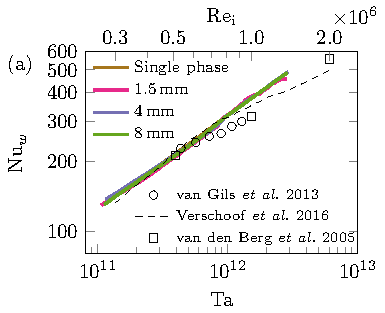
\includegraphics{figure2a.pdf}%
  \label{fig:TaNuwSize}
}%
\subfloat{%
    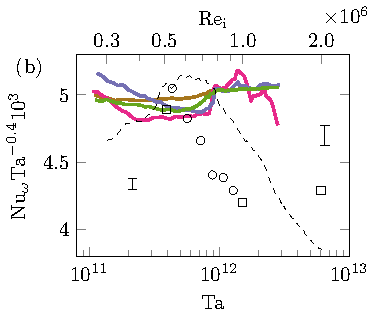
\includegraphics{figure2b.pdf}
  \label{fig:TaNuwTaSize}
}%
\caption{%
(a) $\Nus_\omega (\Tay)$ for \SI{2}{\percent} particle volume fraction with
particle diameters of \SI{1.5}{\milli\metre}, \SI{4.0}{\milli\metre}, and
\SI{8.0}{\milli\metre}, and for comparison the single phase case. Data from
comparable bubbly drag reduction studies are plotted using black markers. (b)
Same data, but now as compensated plot $\Nus_\omega / \Tay^{0.40}$ as function
of $\Tay$.   The error bar indicates the maximum deviation for repeated
measurements from all measurements combined (coloured curves) which is less
than \SI{1}{\percent}. At $\Tay \geq \num{2e12}$, the \SI{1.5}{\milli\metre}
particles show an increased uncertainty of \SI{1.7}{\percent}, which is
indicated by the right error bar.}
\label{fig:dragReductionSize}
\end{figure}
%
\indent Below $\Tay^*$, the drag reduction due to spherical particles appears to be
similar to bubbly drag reduction~\citep{vanGils2013}. However, in the lower
$\Tay$ regime, the bubble distribution was highly non-uniform due to buoyancy
of the bubbles~\citep{vandenBerg2005,vanGils2013,Verschoof2016}. Therefore,
the volume fractions reported were only the global values, and the torque
measurements were for the mid-sections of their setups. What is evident from
the above comparisons is that in the high $\Tay$ regime, air bubbles
drastically reduce the drag, reaching far beyond the drag modification by
rigid spheres.
\newpage
\subsection{Effect of particle volume fraction}\label{subsec:volumeFraction}
The next step is to investigate the effect of the particle volume fraction on
the torque. For the \SI{8}{\milli\metre} particles, we have the ability to
increase the particle volume fraction up to \SI{6}{\percent}. This was done in
steps of \SI{2}{\percent}, and the results are plotted in compensated form in
\reff{fig:TaNuwTaVF}. The normalised torque increases with the volume
fraction of particles. The \SI{6}{\percent} case shows the largest drag.
\refF{fig:TadrVF} shows the same data in terms of drag reduction as
function of $\Tay$. A \SI{2}{\percent} volume fraction of particles gives the
highest drag reduction. With increasing $\alpha$ the drag reduction decreases.
These measurements are in contrast with the findings for bubbly drag
reduction~\citep{vanGils2013}, for which the net drag decreases with
increasing gas volume fraction.
of drag in a particle-laden flow is the larger apparent viscosity.  If we
would calculate the apparent viscosity for our case with the Einstein relation
(\refe{eq:einstein}) for $\alpha=\SI{6}{\percent}$, the drag increase
would be \SI{15}{\percent}, as compared to the pure working fluid.  Including
this effect in our drag reduction calculation would result in reductions of
the same order.  However, when comparing the drag with or without particles,
the \emph{net} drag reduction is practically zero. This result is different
from the work a in turbulent channel flow where they found
that the drag increased more than the increase of the viscosity\citep{Picano2015}.

\begin{figure}
\centering%
\subfloat{%
    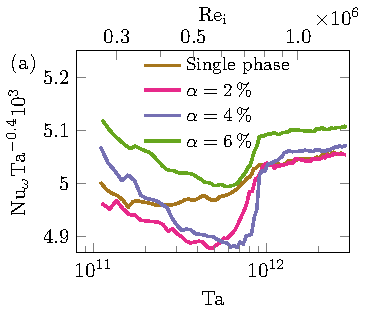
\includegraphics{figure3a.pdf}%
  \label{fig:TaNuwTaVF}
}%
\subfloat{%
    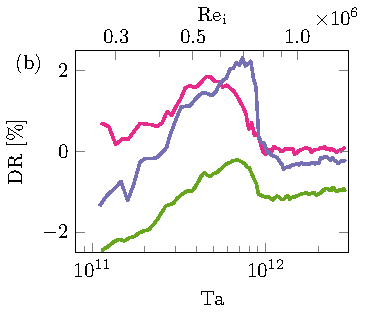
\includegraphics{figure3b.pdf}
  \label{fig:TadrVF}
}%
\caption{%
(a) $\Nus_\omega (\Tay)$, compensated by $\Tay^{0.4}$, for
\SI{8}{\milli\metre} particles with various particle volume fractions and for
comparison the single phase case.  (b) Drag reduction, defined as
$\text{DR} = \left(1 - \Nus_\omega(\alpha) / \Nus_\omega(\alpha=0) \right)$,
plotted against $\Tay$.
}
\label{fig:dragReductionVF}
\end{figure}

For a better comparison with bubbly drag reduction, we plot the drag reduction
as a function of (gas or particle) volume fraction $\alpha$; see 
\reff{fig:alphaDrAll}. Different studies are shown using different symbols, and
$\rey$ is indicated by colours. None of the datasets were compensated for the
changes in effective viscosity.   DR is defined in slightly differently
way in each study: van~den~Berg \citep{vandenBerg2005} makes use of the friction coefficient
$\left(1 - c_f(\alpha) /c_f(0) \right)$; van~Gils \citep{vanGils2013} uses the
dimensionless torque $G=\tau / (2 \pi L_{mid} \rho \nu^2)$, $\left(1 -
G(\alpha) / G(0) \right)$; and Verschoof \citep{Verschoof2016} uses the plain torque
value $\left(1 - \tau(\alpha) /\tau(0) \right)$. While the rigid particles
only showed marginal drag reduction, some studies using bubbles achieve
dramatic reduction of up to \SI{30}{\percent} and beyond. 
\refF{fig:alphaDrZoom} shows a zoomed in view of the bottom part of the plot
with the rigid sphere data. The triangles denote the data from
Verschoof \citep{Verschoof2016}, corresponding to small bubbles in the Taylor-Couette
system. The rigid particles and the small bubbles show a similar drag
response. What is remarkable is that this occurs despite the huge difference
in size. The estimated diameter of the bubbles in Verschoof \citep{Verschoof2016} is
\SI{0.1}{\milli \metre}, while the rigid spheres are about two orders in
magnitude larger. This provides key evidence that the particle size alone is
not enough to cause drag reduction, also the density ratio of the
particle and the carrier fluid is of importance.

\begin{figure}
\centering%
\subfloat{%
    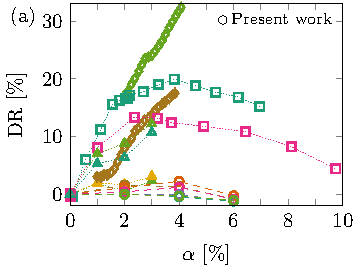
\includegraphics{figure4a.pdf}%
  \label{fig:alphaDrAll}
}%
\subfloat{%
    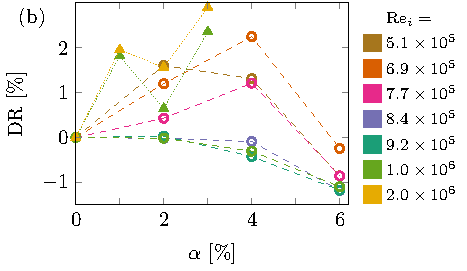
\includegraphics{figure4b.pdf}%
  \label{fig:alphaDrZoom}
}%
\caption[]{(a) Drag reduction as function of particle volume fraction from
    \marksymbol{o}{black}\,: $d_p=\SI{8}{\milli\metre}$ particles from
    present work compared to similar gas volume fractions from
    \marksymbol{square}{black}\,: van~den~Berg\citep{vandenBerg2005},
    \marksymbol{diamond}{black}\,: van~Gils\citep{vanGils2013}, and
    \marksymbol{triangle}{black}\,: Verschoof\citep{Verschoof2016}. Symbols indicate the
    different studies while colours differentiate between the Reynolds
    numbers. The current work has DR defined as $\left(1 -
        \Nus_\omega(\alpha) / \Nus_\omega(\alpha=0) \right)$; the other
        studies use dimensionless torque $G$ \citep{vanGils2013}, friction
        coefficient $c_f$ \citep{vandenBerg2005}, or plain torque $\tau$
        \citep{Verschoof2016} to define DR. (b) Zoom of the bottom part of
    (a) where the data from the present work is compared to bubbly drag
reduction data using \SI{6}{ppm} of surfactant \citep{Verschoof2016}}
\label{fig:dragReductionAlpha}
\end{figure}

\subsection{Effect of marginal changes in particle density ratio}
With the effects of particle size and volume fraction revealed, we next
address the sensitivity of the drag to marginal variations in particle
density. A change in the particle density ratio brings about a change in the
buoyancy and  centrifugal forces on the particle, both of which can affect the
particle distribution within the flow. We tune the particle to fluid density
ratio $\phi \equiv \rho_p/\rho_f$ by changing the volume fraction of glycerol
in the fluid, such that the particles are marginally buoyant ($\phi = 0.94,
0.97$), neutrally buoyant ($\phi=1.00$) and marginally heavy ($\phi=1.04$)
particles. In \reff{fig:TaNuwTaDen} we show the compensated
$\Nus_\omega$ as function of $\Tay$ for various $\phi$. $\alpha$ was fixed to
\SI{6}{\percent} and only \SI{8}{\milli\metre} particles were used. The darker
shades of colour correspond to the single phase cases, while lighter shades
correspond to particle-laden cases. In general, the single phase drag is
larger as compared to the particle-laden cases. However, there is no striking
difference between the different $\phi$.  In \reff{fig:TaDrDen}, we
present the drag reduction for particle-laden cases at different density
ratios. On average we see for all cases drag modification of approximately
$\pm$ \SI{2}{\percent}. We can also identify a small trend in the lower $\Tay$
region: the two larger $\phi$ (heavy and neutrally buoyant particles) tend to
have a drag increase, while the smaller $\phi$ cases (both light particles)
have a tendency for drag reduction. Nevertheless, the absolute difference in
DR between the cases is within 4\%. The above results provide clear evidence
that minor density mismatches do not have a serious influence on the global
drag of the system.  To investigate for strong buoyancy effects,
additional measurements were done using \SI{2}{\milli\metre} expanded
polystyrene particles ($\phi=0.02$).  However, due to the particles
accumulating between the inner cylinder segments leading to additional
mechanical friction, these measurements were inconclusive.

\begin{figure}
\centering
\subfloat{
    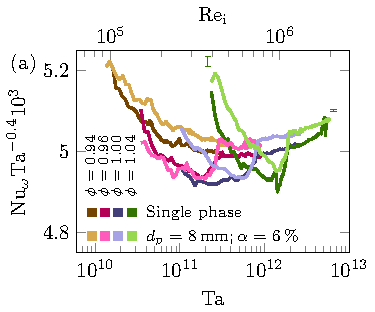
\includegraphics{figure5a.pdf}
  \label{fig:TaNuwTaDen}
}
\subfloat{
    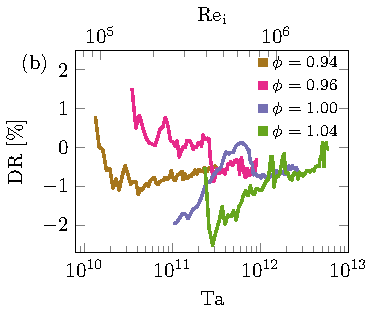
\includegraphics{figure5b.pdf}
  \label{fig:TaDrDen}
}
\caption{
(a) $\Tay$ as function of $\Nus_\omega$ compensated by $\Tay^{0.4}$ for
various density ratios $\phi=\rho_p/\rho_f$ indicated by the corresponding
colour. The darker shades indicate the single phase cases while the
lighter shades show the cases using \SI{6}{\percent} particle volume
fraction of \SI{8}{\milli\metre} diameter particles. Due to the increase
in viscosity the maximum attainable $\Tay$ is lower for larger density
ratios. The uncertainty is again estimated using the maximum
deviation from the average for multiple runs and here only shown for
the green curves. This value is slightly below \SI{1}{\percent} at
lower $\Tay$ and decreases with increasing $\Tay$ to values below
\SI{0.25}{\percent}. This trend is seen for all $\phi$.  (b) 
Drag reduction, calculated from the data of figure 5a, plotted against
$\Tay$. The drag reduction is defined as $\text{DR} = \left(1 -
\Nus_\omega(\alpha=6\%) / \Nus_\omega(\alpha=0) \right)$.
}
\label{fig:dragReductionDen}
\end{figure}
\newpage
\subsection{Flow statistics using particles} 
In the above sections, we presented the effects of changing particle size,
volume fraction, and density on the global drag of the system. Next we look
into local flow
properties using LDA while the particles are present.  First, we collected a
total of \num{1e6} data points of azimuthal velocity at mid-height and
mid-gap.  These were captured over a period of approximately $\num{3e4}$
cylinder rotations. From this data we calculate the probability density
function (PDF) of $\text{u}_\theta$ normalised by $u_i$ for various $\alpha$,
shown in \reff{fig:U_w_pdf}. The particle size was fixed to
\SI{8}{\milli\metre} and the Reynolds number was set to $\num{1e6}$. From this
figure we see a large increase in turbulent fluctuations, resulting in very
wide tails. While the difference between \SI{2}{\percent}, \SI{4}{\percent},
and \SI{6}{\percent} is not large, we can identify an increase in fluctuations
with increasing $\alpha$. These increased fluctuations can be explained by the
additional wakes produced by the particles \citep{Poelma2007,Almeras2017}. The
increase in fluctuations can also be visualized using the standard deviation
of $\sigma(u_\theta) = \left< \text{u}_\theta'^2 \right>^{1/2}$ normalised by
the standard deviation of the single phase case---see 
\reff{fig:alpha_u_rms_u0}. In this figure, $\sigma(u_\theta)$ is shown for
three different $\rey$, again for \SI{8}{\milli\metre} particles. In general,
we see a monotonically increasing trend with $\alpha$, and it seems to
approach an asymptotic value. One can speculate that there has to be an upper
limit for fluctuations which originate from wakes of the particles. For large
$\alpha$ the wakes from particles will interact with each other and with the
carried flow.

\begin{figure}
\centering%
\subfloat{%
    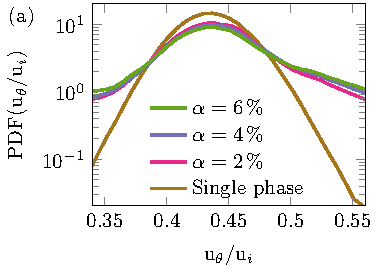
\includegraphics{figure6a.pdf}%
  \label{fig:U_w_pdf}
}%
\subfloat{%
    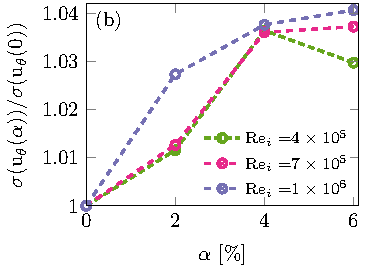
\includegraphics{figure6b.pdf}%
  \label{fig:alpha_u_rms_u0}
}%
\caption{%
(a) PDF of $\text{u}_\theta / \text{u}_i$ for various $\alpha$ and the
single phase case. The particle size was fixed to \SI{8}{\milli\metre}
and $\rey_i=\num{1e6}$ for all cases. (b) Standard deviation of the
azimuthal velocity normalized by the standard deviation of the single phase
case for three different $\rey$ for a fixed particle size of
\SI{8}{\milli\metre}.} \label{fig:ldaresults}
\end{figure}

Measurements using \SI{4}{\milli\metre} particles yielded qualitatively
similar results. It is known that in particle-laden gaseous pipe flows, large
particles can increase the turbulent fluctuations, while small particles
result in turbulence attenuation \citep{Tsuji1984,Gore1989,Vreman2015}. The
LDA measurements were not possible with the smallest particles
(\SI{1.5}{\milli\metre}), as the large amount of particles in the flow blocked
the optical paths of the laser beams.

We are confident that for these bi-disperse particle-laden LDA measurements,
the large particles do not have an influence on the measurements as these
\emph{millimetric}-sized particles are much larger than the fringe spacing
($d_f = \SI{3.4}{\micro\metre}$) and do not show a Doppler burst.  However,
during the measurements the particles get damaged and small bits of material
are fragmented off the particles. We estimate the size of these particles
slightly larger than the tracer particles and these can have an influence on
the LDA measurements as they do not act as tracers.

How the average azimuthal velocity changes with particle radius is shown in
\reff{fig:ldaradial}.  We measured a total of $\num{3e4}$ data points
during approximately 900 cylinder rotations. Again, the data were corrected
for velocity bias by using the transit time as a weighing factor. 
\refF{fig:U_theta_radius_size} shows the effect of particle size for
$\alpha=\SI{2}{\percent}$, and \reff{fig:U_theta_radius_vol} shows the
effect of particle volume fraction for \SI{8}{\milli\metre} particles. Both
figures additionally show the high-precision single phase data from another
study \citep{Huisman2013} for which our single phase measurements are practically
overlapping. Since LDA measurements close to the inner cylinder are difficult,
due to the reflecting inner cylinder surface, we limited our radial extent to
$\tilde{r}=(r - r_i) / (r_o - r_i)=[0.2,1]$. We found that the penetration
depth of our LDA measurements is the smallest for experiments with the
smallest particles and the largest $\alpha$. All differences with the single
phase case are only marginal and we can conclude that the average mean
velocity is not much affected by the particles in the flow, at least for
$\tilde{r} \geq 0.2$.

\begin{figure}
\centering%
\subfloat{%
    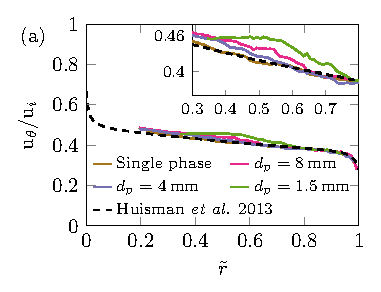
\includegraphics{figure7a.pdf}%
  \label{fig:U_theta_radius_size}
}%
\subfloat{%
    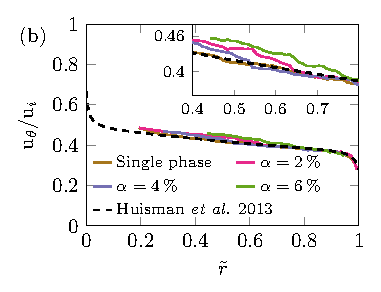
\includegraphics{figure7b.pdf}%
  \label{fig:U_theta_radius_vol}
}%
\caption{%
$\text{u}_\theta$ normalised by the velocity of the inner cylinder wall
$\text{u}_i$ as function of the normalised radius for various $d_p$ while
$\alpha=\SI{2}{\percent}$ (a) and various $\alpha$ while
$d_p=\SI{8}{\milli\metre}$ (b). In all cases $\rey_i$ is fixed to $\num{1e6}$.
For comparison, the single phase case using water at $\rey_i=\num{1e6}$ from
Huisman~\citep{Huisman2013} is also plotted in dashed black in both plots. Both figures
have an inset showing an enlargement of the centre area from the same
figure.} \label{fig:ldaradial}
\end{figure}

\begin{figure}
\centering%
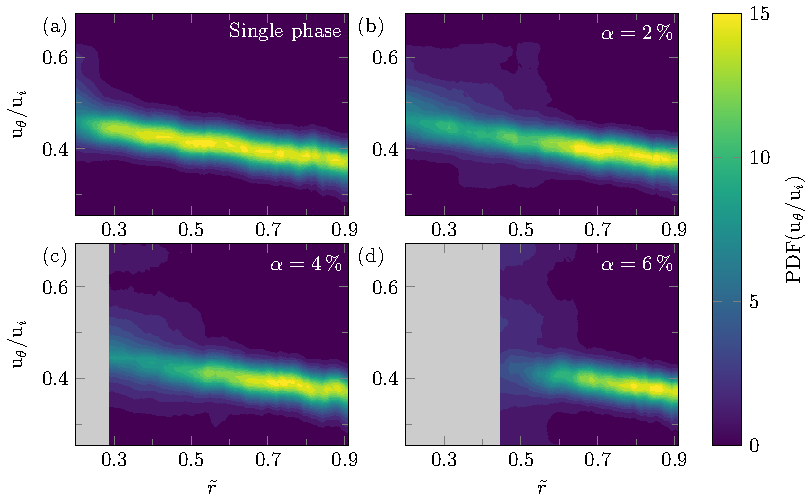
\includegraphics{figure8.pdf}%
\caption{%
\label{fig:heatmap}
PDF of the normalised azimuthal velocity as a function of normalised radial
position for various $\alpha$ for the case of \SI{8}{\milli\metre} particles
and the single phase case while keeping $\rey$ at $\num{1e6}$. With increasing
$\alpha$ the maximum penetration depth decreases. The grey areas indicate
radial positions for which no data is available.
}
\end{figure}

To get an idea of the fluctuations we can use the previous data to construct a
two-dimensional PDF of the azimuthal velocity as function of radius. These are
shown for $\rey = \num{1e6}$ using \SI{8}{\milli\metre} particles at various
$\alpha$ and the single phase case in \reff{fig:heatmap}.  First thing
to notice is again that the penetration depth is decreasing with increasing
$\alpha$.  The single phase case shows a narrow banded PDF. When $\alpha$ is
increased, for the lower values of $\tilde{r}$ the PDF is much wider.  While
it makes sense that an increase in $\alpha$ increases the fluctuations due to
the increased number of wakes of particles, this is expected everywhere in the
flow, not only closer to the inner cylinder.  It is possible that the
particles have a preferred concentration closer to the inner cylinder.  We
have tried to measure the local concentration of particles as function of
radius but failed due to limited optical accessibility.  Therefore, we can
only speculate under what circumstances there would be an inhomogeneous
particle distribution which would lead to the visible increase in
fluctuations.  The first possibility is a mismatch in density between the
particle and the fluid, which would result in light particles ($\phi < 1$) to
accumulate closer to the inner cylinder.  Another possibility is that due to
the rotation of the particle, an effective lift force arises, leading to a
different particle distribution in the flow. While this is quite plausible,
this is difficult to validate as we would need to capture the rotation.  The
fragments of plastic that are sheared off the particles can also have a bias
to the LDA measurement. While we estimate them to be larger than the tracers,
they might still be small enough to produce a signal and they might not follow
the flow faithfully.

\section{Conclusions and outlook}\label{sec:conclusions_and_outlook}
We have conducted an experimental study on the drag response of a highly
turbulent Taylor-Couette flow containing rigid neutrally buoyant spherical
particles. We have found that, unlike the case of bubbles used in prior
works~\citep{vanGils2013,Verschoof2016}, rigid particles barely reduce (or
increase) the drag on the system, even for cases where their size was
comparable to that of bubbles used in other studies.
There was no significant size effect. Even for very large particles, which can
attenuate turbulent fluctuations and generate wakes, there was no distinct
difference with the single phase flow.
We also varied the volume fraction of the particles in the range 0\%--6\%. The
particle volume fraction has no greater effect on the system drag than what is
expected due to changes in the apparent viscosity of the suspension. Further,
we tested the sensitivity of our drag measurements to marginal variations in
particle to fluid density ratio $\phi$. A trend was noticeable, towards drag
reduction when $\phi$ was reduced from 1.00 to 0.94. This suggests that a low
density of the particle could be a necessary ingredient for drag reduction.
Finally, we have also probed the local flow at the mid height and mid gap of
the system using LDA. With the addition of particles, the liquid velocity
fluctuations are enhanced, with wider tails of the distributions. A finite
relative velocity between the particle and the flow around it can cause this
increase in velocity fluctuations~\citep{Mathai2015}, as seen for bubbly flows
(pseudo-turbulence), and in situations of sedimenting particles in quiescent
or turbulent environments~\citep{Gore1989}.  In the present situation, the
relative velocity between the particle and the flow is expected, owing to the
inertia of the finite-sized particles we used.
There is only a marginal deviation from the single phase case in the average
azimuthal velocity over the radial positions measured using any size or
concentration of particles measured. From the two-dimensional PDFs, we see
that closer to the inner cylinder, using smaller $d_p$ or larger $\alpha$, the
PDF gets wider. This can be due to a preferential concentration of the
particles or a slight density mismatch.

\textcolor{black}{Our study is a step towards a better understanding of the
mechanisms of bubbly drag reduction. Bubbles are deformable, and they have
a tendency to migrate towards the walls, either due to lift
force~\citep{Dabiri2013}, or due to the centripetal
effects~\citep{vanGils2013}. When compared to the drag reducing bubbles 
\citep{vanGils2013,Verschoof2016}, our particles do not deform, and they do
not experience centripetal effects as they are density matched.  At
least one of these differences must therefore be crucial for the observed,
bubbly drag reduction in those experiments.
In a future investigation, we will conduct more experiments using very light
spherical particles that experience similar centripetal forces as the bubbles
in van~Gils~\citep{vanGils2013}, but are non-deformable.} These particle need to be
larger than the size of the gap between the inner cylinder segments and very
rigid, or the setup needs to be modified to close the gap between the IC
segments.  Such experiments can then disentangle the role of particle density
on drag reduction from that of the particle shape.

\graphicspath{{fig/}}

   % Spheres
%%%%%%%%%%%%%%%%%%%%%%%%%%%
%%% Chapter definitions %%%
%%%%%%%%%%%%%%%%%%%%%%%%%%%
% Chapter title
\renewcommand{\mychaptertitle}{%
Finite-sized rigid spheres in turbulent Taylor-Couette flow: %
Effect on the overall drag%
}
% Chapter short title
\renewcommand{\mychaptershorttitle}{%
Finite-sized rigid spheres in turbulent Taylor-Couette flow%
}
% Chapter authors
\renewcommand{\mychapterauthors}{%
\textbf{Dennis~Bakhuis},
Ruben~A.~Verschoof,
Varghese~Mathai,
Sander~G.~Huisman,
Detlef~Lohse,
and
Chao~Sun
\textit{Finite-sized rigid spheres in turbulent Taylor-Couette flow:
Effect on the overall drag},
J. Fluid Mech. \textbf{850}, 246--261 (2018).
}
% Chapter abstract
\renewcommand{\mychapterabstract}{%
We report on the modification of drag by neutrally buoyant spherical
finite-sized particles in highly turbulent Taylor-Couette (TC) flow.  These
particles are used to disentangle the effects of size, deformability, and
volume fraction on the drag, and are contrasted with the drag in bubbly TC
flow.  From global torque measurements we find that rigid spheres hardly
decrease or increase the torque needed to drive the system.   The size of the
particles under investigation have a marginal effect on the drag, with smaller
diameter particles showing only slightly lower drag.  Increasing the particle
volume fraction shows a net drag increase, however this increase is much
smaller than can be explained by the increase in apparent viscosity due to the
particles.  The increase in drag for increasing particle volume fraction is
corroborated by performing laser Doppler anemometry where we find that the
turbulent velocity fluctuations also increase with increasing volume fraction.
In contrast with rigid spheres, for bubbles the effective drag reduction also
increases with increasing Reynolds number. Bubbles are also much more
effective in reducing the overall drag. 
}
\renewcommand{\mychaptermark}{Neutrally buoyant spheres}
\renewcommand{\mychapterlabel}{chap:spheres}
\renewcommand{\mychaptericon}{fig/swchapter1.png}
%%%%%%%%%%%%%%%%%%%%%%%%%%%%%
%%% Create Chapter Header %%%
%%%%%%%%%%%%%%%%%%%%%%%%%%%%%
%%%%%%%%%%%%%%%%%%%%%%
%%% Chapter header %%%
%%%%%%%%%%%%%%%%%%%%%%
\globalcolor{ChapterText}
\chapter[\mychaptershorttitle]{%
    \mychaptertitle%
    \ifdefined\starwarsfootnotes
        \textsuperscript{%
            \hspace{-1mm}%
            \includegraphics[height=\swsymsize]{\mychaptericon}%
        }%
        \blfootnote{%
            \textcolor{footnotetextcolor}{%
                \textsf{%
                    \vspace{0.5mm}\hspace{-1mm}%
                    \includegraphics[height=\swfnsymsize]{\mychaptericon}%
                    \hspace{0.5mm}%
                    Based on: \mychapterauthors%
                }
            }
        }
    \else
        \footnote{\textsf{%
             Based on: \mychapterauthors%
        }}%
    \fi
}
\pagecolor{ChapterBackground}
\afterpage{\pagecolor{White}\globalcolor{Black}} 
\label{\mychapterlabel}
\chaptermark{\mychaptermark}
\noindent\rule{\textwidth}{0.4pt}%
\vspace{0.2cm}
\noindent\textsf{\mychapterabstract}
\clearpage

%%%%%%%%%%%%%%%%%%%%%%%%
%%%% end title page %%%%
%%%%%%%%%%%%%%%%%%%%%%%%
\graphicspath{{ChapterOne/fig/}}
\section{Introduction}
Flows in nature and industry are generally turbulent, and often these flows
carry bubbles, drops, or particles of various shapes, sizes, and densities.
Examples include sediment-laden rivers, gas-liquid reactors, volcanic
eruptions, plankton in the oceans, pollutants in the atmosphere, and air
bubbles in the ocean mixing layer~\citep{Toschi2009}.  Particle-laden flows
may be characterized in terms of particle density $\rho_p$, particle diameter
$d_p$, volume fraction $\alpha$, and Reynolds number Re of the flow. When
$d_p$ is small (compared to the dissipative length scale $\eta_K$) and
$\alpha$ low ($< 10^{-3}$), the system may be modelled using a point particle
approximation with two-way
coupling~\citep{Elghobashi1994,Mazzitelli2003,Mathai2016}.  With recent
advances in computing, fully resolved simulations of particle-laden flows have
also become feasible.  Uhlmann conducted one of the first numerical
simulations of finite-sized rigid spheres in a vertical particle-laden channel
flow \citep{Uhlmann2008}.  They observed a modification of the mean velocity
profile and turbulence modulation due to the presence of particles. A number
of studies followed, which employed immersed
boundary~\citep{Peskin2002,Cisse2013}, Physalis~\citep{Naso2010, Wang2017b},
and front-tracking methods~\citep{Unverdi1992,Roghair2011,Tagawa2013} to treat
rigid particles and deformable bubbles, respectively, in channel and pipe flow
geometries~\citep{Pan1996,Lu2005,Uhlmann2008,Dabiri2013,Kidanemariam2013,Lashgari2014,Picano2015,Costa2016}. 
Flows with dispersed particles, drops, and bubbles can, under the right
conditions, reduce skin friction and result in significant energetic (and
therefore financial) savings. In industrial settings this is already achieved
using polymeric additives which disrupt the self-sustaining cycle of wall
turbulence and dampen the quasi-streamwise vortices
\citep{White2008,Procaccia2008}. Polymeric additives are impractical for
maritime applications, and therefore gas bubbles are used with varying success
rates \citep{Ceccio2010,Murai2014}. Local measurements in bubbly flows are
non-trivial and the key parameters and their optimum values are still unknown.
For example, it is impossible to fix the bubble size in experiments and
therefore to isolate the effect of bubble size. Various studies hinted that
drag reduction can also be achieved using spherical particles
\citep{Zhao2010}, also by using very large particles in a turbulent von
K\'arm\'an flow \citep{Cisse2015}. In this latter study a tremendous decrease
in turbulent kinetic energy (TKE) was observed. A similar, but less intense,
decrease in TKE was also seen using a very low particle volume
fraction\citep{Bellani2012b}. By using solid particles it is possible to
isolate the size effect on drag reduction and even though rigid particles are
fundamentally different from bubbles, this can give additional insight into
the mechanism of bubbly drag reduction.  The particle dynamics are highly
influenced by the diameter of the particle\citep{Machicoane2016}. This might
or might not have a direct influence on the global drag of the system and has
never been studied.
%
Whether and when solid particles increase or decrease the drag in a flow is
yet not fully understood and two lines of thought exist. On one side, it is
hypothesized that solid particles {\it decrease} the overall drag as they damp
turbulent fluctuations \citep{Zhao2010,Poelma2007}. On the other side, one
could expect that solid particles {\it increase} drag as they shed vortices,
which must be dissipated. In addition, they also increase the apparent
viscosity. A common way to quantify this is the so called `Einstein
relation'~\citep{Einstein1906}
\begin{equation} \nu_\alpha = \nu\left(1 +
\frac{5}{2}\alpha \right), \label{eq:einstein} \end{equation} where $\nu$ is
the viscosity of the continuous phase. This compensation is valid for the
small $\alpha$ values used in this \docname \citep{Stickel2005}. Direct
measurements of drag in flows with solid particles are scarce, and the debate
on under what condition they either enhance or decrease the friction has not
yet been settled. Particles and bubbles may show collective effects
(clustering) and experiments have revealed that this has significant influence
on the flow properties~\citep{Liu1993, Kulick1994, Muste1997, So2002,
Fujiwara2004, vandenBerg2005, vandenBerg2007, Shawkat2008, Calzavarini2008,
Colin2012, vanGils2013, Maryami2014, Mathai2015,
Almeras2017,Mathai2018}. In general, the Stokes number is used to
predict this clustering behaviour, but for neutrally buoyant particles this is
found to be insufficient \citep{Bragg2015,Fiabane2012}. In addition, the
position of the particles (or the particles clusters) is likely to have a
large influence on the skin friction.  It was shown in DNS at low Reynolds
numbers, that the particle distribution is mainly
governed by the bulk Reynolds number\citep{Kazerooni2017}.

In order to study the effects of particles on turbulence it is convenient to
use a closed setup where one can relate global and local quantities directly
through rigorous mathematical relations. In this \docname the Taylor-Couette
(TC) geometry~\citep{Grossmann2016}---the flow between two concentric rotating
cylinders---is employed as this is a closed setup with global balances. The
driving of the Taylor-Couette geometry can be described using the Reynolds
number based on the inner cylinder (IC): $\rey_i = u_i d / \nu$, where $u_i =
\omega_i r_i$ is the azimuthal velocity at the surface of the IC, $\omega_i$
the angular velocity of the IC, $d = r_o - r_i$ the gap between the cylinders,
$\nu$ the kinematic viscosity, and $r_i$($r_o$) the radius of the inner(outer)
cylinder. The geometry of Taylor-Couette flow is characterized by two
parameters: the radius ratio $\eta=r_i/r_o$ and the aspect ratio $\Gamma =
L/d$, where $L$ is the height of the cylinders. The response parameter of the
system is the torque, $\tau$, required to maintain constant rotation speed of
the inner cylinder. It was mathematically shown that in Taylor-Couette flow
the angular velocity flux defined as $J^\omega = r^3 \left(  \left
\langle u_r \omega \right \rangle_{A,t} - \nu \frac{\partial} {\partial r}
\left \langle \omega \right \rangle_{A,t} \right)$, where the subscript $A,t$
denotes averaging over a cylindrical surface and time,	is a radially
conserved quantity (Eckhardt, Grossmann, Lohse \citep{Eckhardt2007} (EGL)). One can, in analogy to
Rayleigh-B\'enard convection, normalize this flux and define a Nusselt number
based on the flux of the angular velocity:
\begin{equation}
  \Nus_\omega = \frac{J^\omega}{J^\omega_{\text{lam}}} = \frac{\tau}{2 \pi L \rho J^\omega_{\text{lam}}},
\end{equation}
where $J^\omega_{\text{lam}} = 2 \nu r^2_i r^2_o \left( \omega_i - \omega_o
\right)/\left( r^2_o - r^2_i \right)$ is the angular velocity flux for
laminar, purely azimuthal flow and $\omega_o$ is the angular velocity of the
outer cylinder. In this spirit the driving is expressed in terms of the Taylor
number:
\begin{equation}
  \Tay = \frac{1}{4} \sigma d^2 \left(r_i + r_o \right)^2 \left( \omega_i - \omega_o \right)^2 \nu^{-2}.
\end{equation}
Here $\sigma = \left( \left( 1 + \eta \right) / \left(2 \sqrt{\eta} \right)
\right)^4\;\approx\;1.057$ is a geometric parameter (``geometric Prandtl
number''), in analogy to the Prandtl number in Rayleigh-B\'enard convection.
In the presented work, where only the inner cylinder is rotated and the outer
cylinder is kept stationary, we can relate $\Tay$ to the Reynolds number of
the inner cylinder by
\begin{equation}
\rey_i = \frac{r_i \omega_i d}{\nu} = \frac{8\eta^2}{(1+\eta)^{3}} \sqrt{\Tay}.
\end{equation}
\noindent The scaling of the dimensionless angular velocity flux (torque) with
the Taylor (Reynolds) number has been analysed extensively, see e.g.
\citep{Lathrop1992,Lewis1999,Paoletti2011,vanGils2011,Ostilla-Monico2013} and
the review articles \citep{Fardin2014,Grossmann2016}, and the
different regimes are well understood. In the current Taylor number regime it
is known that $\Nus_\omega \propto \Tay^{0.4}$. Because this response is
well known, it can be exploited to study the influence of immersed bubbles and
particles
~\citep{vandenBerg2005,vandenBerg2007,vanGils2013,Maryami2014,Verschoof2016}
on the drag needed to sustain constant rotational velocity of the inner
cylinder. 

In this \docname we will use the TC geometry to study the effect of neutrally
buoyant rigid spherical particles on the drag. We study the effects of varying
the particle size $d_p$, the volume fraction $\alpha$, the density ratio
$\phi$, and the flow Reynolds number $\text{Re}$ on the global torque (drag)
of the Taylor-Couette flow. The drag reduction is expressed as $\text{DR} =
\left(1 - \Nus_\omega(\alpha) / \Nus_\omega(\alpha=0) \right)$ and as we are
interested in the net drag reduction, it is \emph{not} compensated for
increased viscosity effects using correction models, such as the Einstein
relation.

The \docname is organized as follows. \refSec{sec:experimentalSetup}
presents the experimental setup. In \refsec{sec:sphereresults} we discuss the
results. The findings are summarized and an outlook for future work is given
in the last section.

\section{Experimental setup}\label{sec:experimentalSetup}
The experiments were conducted in the Twente Turbulent Taylor-Couette
(T${}^3$C) facility \citep{vanGils2011}. A schematic of the setup is shown in
\reff{fig:setup}. In this setup, the flow is confined between two
concentric cylinders, which rotate independently. The top and bottom plates
are attached to the outer cylinder. The radius of the inner cylinder (IC) is
$r_i = \SI{0.200}{\metre}$ and the radius of the outer cylinder (OC) is $r_o =
\SI{0.2794}{\metre}$, resulting in a gap width of $d = r_o - r_i =
\SI{0.0794}{\metre}$ and a radius ratio of $\eta = r_i/r_o = 0.716$. The IC
has a total height of $L = \SI{0.927}{\metre}$ resulting in an aspect ratio of
$L / d = 11.7$. The IC is segmented axially in three parts. To minimize the
effect of the stationary end plates, the torque is measured only over the
middle section of the IC with height $L_{\text{mid}}/L = 0.58$, away from
the end plates. A hollow reaction torque sensor made by Honeywell is used to
measure the torque which has an error of roughly 1\% for the largest torques
we measured. Between the middle section and the top and bottom section of the
inner cylinder is a gap of 2mm.

The IC can be rotated up to $f_i = \omega_i/(2\pi) =
\SI{20}{\hertz}$. In these experiments only the IC is rotated and the OC is
kept at rest. The system holds a volume of $V = \SI{111}{\litre}$ of working
fluid, which is a solution of glycerol ($\rho =
\SI{1260}{\kilo\gram/\metre\cubed}$) and water. To tune the density of the
working fluid, the amount of glycerol was varied between \SI{0}{\percent} and
\SI{40}{\percent} resulting in particles being marginally heavy,
neutrally buoyant, or marginally light.
\begin{figure}
\centering
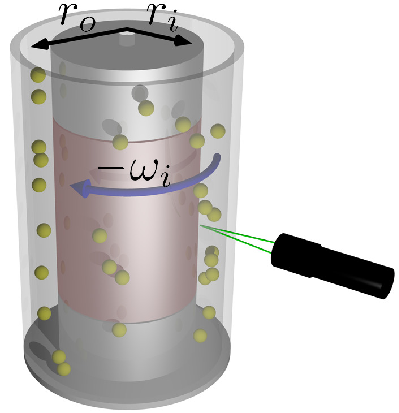
\includegraphics[height=5.5cm]{figure1.pdf}
\caption{
Schematic of the Taylor-Couette setup. Two concentric cylinders of radii
$r_{i,o}$ with a working fluid in between. Particles are not to scale. The
inner cylinder rotates with angular velocity $\omega_i$, while the outer
cylinder is kept at rest. We measure the torque on the middle section
(highlighted). The laser Doppler anemometry (LDA) probe is positioned at mid
height to measure the azimuthal velocity at mid gap.}
\label{fig:setup}
\end{figure}
The system is thermally controlled by cooling the top and bottom plates of the
setup. The temperature was kept at $T = \SI{20(1)}{\celsius}$ for all the
experiments, with a maximum spatial temperature difference of
$\SI{0.2}{\kelvin}$ within the setup, and we account for the density and
viscosity changes of water and glycerol \citep{Glycerine1963}.

Rigid polystyrene spherical particles (\textit{RGPballs S.r.l.}) were used in
the experiments, these particles have a density close to that of water
(940\,--\SI{1040}{\kilo\gram/\metre\cubed}). We chose particles with diameters
$d_p = 1.5$, 4.0, and $\SI{8.0}{\milli\metre}$. To our disposal are:
\SI{2.22}{\litre} of \SI{1.5}{\milli\metre} diameter particles,
\SI{2.22}{\litre} of \SI{4}{\milli\metre} diameter particles, and
\SI{6.66}{\litre} of \SI{8}{\milli\metre} diameter particles, resulting in
maximum volume fractions of \SI{2}{\percent}, \SI{2}{\percent}, and
\SI{6}{\percent}, respectively. The particles are found to be nearly
mono-disperse (\SI{99.9}{\percent} of the particles are within \SI{\pm
0.1}{\milli\metre} of their target diameter). Due to the fabrication process,
small air bubbles are sometimes entrapped within the particles. This results
in a slight heterogeneous density distribution of the particles. After
measuring the density distribution for each diameter, we calculated the
average for all batches, which is $\rho_p = \SI{1036 \pm
5}{\kilo\gram/\metre\cubed}$. By adding glycerol to water we match this value
in order to have neutrally buoyant particles.

Using a laser Doppler anemometry (LDA) system (BSA F80, Dantec Dynamics) we
captured the azimuthal velocity at mid-height and mid-gap of the system (see
\reff{fig:setup}) and we performed a radial scan at mid-height.
The flow was seeded with \SI{5}{\micro\metre} diameter polyamide particles
(PSP-5, Dantec Dynamics). Because of the curved surface of the outer cylinder
(OC), the beams of the LDA get refracted in a non-trivial manner, which was
corrected for using a ray-tracing technique \citep{Huisman2012}. 

Obviously, LDA measurements in a multi-phase flow are more difficult to set up
than for single phase flows, as the method relies on the reflection of
light from tiny tracer particles passing through a measurement volume
($\SI{0.07}{\milli\metre} \times \SI{0.07}{\milli\metre} \times
\SI{0.3}{\milli\metre}$).  Once we add a second type of relatively large
particles to the flow, this will affect the LDA measurements, mostly by
blocking the optical path, resulting in lower acquisition rates. These large
particles will also move through the measurement volume, but as these
particles are at least 300 times larger than the tracers and thus much larger
than the fringe pattern (fringe spacing $d_f=\SI{3.4}{\micro\metre}$), the
reflected light is substantially different from a \emph{regular} Doppler burst
and does not result in a measured value. The minimal signal-to-noise ratio for
accepting a Doppler burst was set to 4. As a post-processing step the
velocities were corrected for the velocity bias by using the transit time of
the tracer particle.
\newpage
\section{Results}\label{sec:sphereresults}
\subsection{Effect of particle size}\label{subsec:sizeEffect}
First we study the effect of changing the particle diameter on the torque of
the system. In these experiments, we kept the particle volume fraction fixed
at \SI{2}{\percent} and the density of the working fluid, $\rho_f$, at
\SI{1036}{\kilogram/\metre \cubed}, for which the particles are neutrally
buoyant. The results of these measurements are presented as
$\Nus_\omega(\Tay)$ in \reff{fig:TaNuwSize}. Our curves are practically
overlapping, suggesting that the difference in drag between the different
particle sizes is only marginal. We compare these with the bubbly drag
reduction data at similar conditions (hollow symbols) 
\citep{Verschoof2016,vanGils2013,vandenBerg2005}. At low $\Tay$ the symbols
overlap with our data. However, at larger $\Tay$, the bubbly flow data shows
much lower torque (drag) than the particle-laden cases. As we are in the
ultimate regime of turbulence where $\Nus_\omega$ effectively scales as
$\Nus_\omega \propto \Tay^{0.4}$~\citep{Huisman2012,Ostilla-Monico2013}, we
compensate the data with $\Tay^{0.40}$ in \reff{fig:TaNuwTaSize} to
emphasize the differences between the datasets. For the single phase
case, this yields a clear plateau. For the particle-laden cases, the lowest
drag corresponds to the smallest particle size. The reduction is however quite
small ($<\SI{3}{\percent}$). The compensated plots also reveal a sudden
increase in drag at a critical Taylor number $\Tay^* =\num{0.8e12}$. The jump
is more distinct for the smaller particles, and might suggest a reorganisation
of the flow \citep{Huisman2014}. Beyond $\Tay^*$, the drag reduction is
negligible for the larger particles (\SI{4}{\milli \metre} and \SI{8}{\milli
\metre} spheres). However, for the \SI{1.5}{\milli\metre} particles, the drag
reduction seems to increase, and was found to be very repeatable in
experiments. Interestingly, the size of these particles is comparable to that
of the air bubbles \citep{vanGils2013}.  This might suggest that for smaller
size particles at larger $\Tay$, one could expect drag reduction. At the
increased viscosity of the suspension, a maximum $\Tay \approx 3 \times
10^{12}$ could be reached in our experiments.   We have performed an
uncertainty analysis by repeating the measurements for the single phase, and
for the cases with \SI{8}{\milli\metre} and \SI{1.5}{\milli\metre} particles
multiple times and calculating the maximum deviation from the ensemble
average.  The left error bar indicates the maximum deviation for all
measurements combined and is $\approx \SI{1}{\percent}$.  For $\Tay \geq
\num{2e12}$, we see an increase in uncertainty of \SI{1.7}{\percent} (shown by
the right error bar in \reff{fig:TaNuwTaSize}), which is only caused by
the \SI{1.5}{\milli\metre} particles. These tiny particles can accumulate in
the \SI{2}{\milli\metre} gap between the cylinder segments and thereby
increase the uncertainty. Above $\Tay \geq \num{2e12}$, both, the
\SI{8}{\milli\metre} and \SI{4}{\milli\metre} particles, show a maximum
deviation below 0.25\%.\\
%
\begin{figure}
\centering%
\subfloat{%
    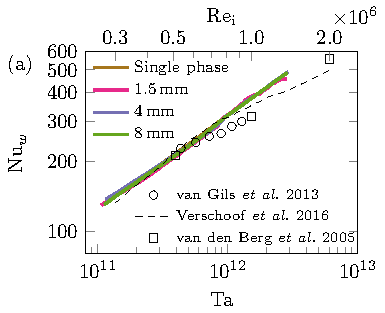
\includegraphics{figure2a.pdf}%
  \label{fig:TaNuwSize}
}%
\subfloat{%
    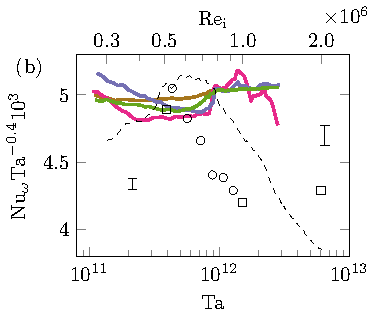
\includegraphics{figure2b.pdf}
  \label{fig:TaNuwTaSize}
}%
\caption{%
(a) $\Nus_\omega (\Tay)$ for \SI{2}{\percent} particle volume fraction with
particle diameters of \SI{1.5}{\milli\metre}, \SI{4.0}{\milli\metre}, and
\SI{8.0}{\milli\metre}, and for comparison the single phase case. Data from
comparable bubbly drag reduction studies are plotted using black markers. (b)
Same data, but now as compensated plot $\Nus_\omega / \Tay^{0.40}$ as function
of $\Tay$.   The error bar indicates the maximum deviation for repeated
measurements from all measurements combined (coloured curves) which is less
than \SI{1}{\percent}. At $\Tay \geq \num{2e12}$, the \SI{1.5}{\milli\metre}
particles show an increased uncertainty of \SI{1.7}{\percent}, which is
indicated by the right error bar.}
\label{fig:dragReductionSize}
\end{figure}
%
\indent Below $\Tay^*$, the drag reduction due to spherical particles appears to be
similar to bubbly drag reduction~\citep{vanGils2013}. However, in the lower
$\Tay$ regime, the bubble distribution was highly non-uniform due to buoyancy
of the bubbles~\citep{vandenBerg2005,vanGils2013,Verschoof2016}. Therefore,
the volume fractions reported were only the global values, and the torque
measurements were for the mid-sections of their setups. What is evident from
the above comparisons is that in the high $\Tay$ regime, air bubbles
drastically reduce the drag, reaching far beyond the drag modification by
rigid spheres.
\newpage
\subsection{Effect of particle volume fraction}\label{subsec:volumeFraction}
The next step is to investigate the effect of the particle volume fraction on
the torque. For the \SI{8}{\milli\metre} particles, we have the ability to
increase the particle volume fraction up to \SI{6}{\percent}. This was done in
steps of \SI{2}{\percent}, and the results are plotted in compensated form in
\reff{fig:TaNuwTaVF}. The normalised torque increases with the volume
fraction of particles. The \SI{6}{\percent} case shows the largest drag.
\refF{fig:TadrVF} shows the same data in terms of drag reduction as
function of $\Tay$. A \SI{2}{\percent} volume fraction of particles gives the
highest drag reduction. With increasing $\alpha$ the drag reduction decreases.
These measurements are in contrast with the findings for bubbly drag
reduction~\citep{vanGils2013}, for which the net drag decreases with
increasing gas volume fraction.
of drag in a particle-laden flow is the larger apparent viscosity.  If we
would calculate the apparent viscosity for our case with the Einstein relation
(\refe{eq:einstein}) for $\alpha=\SI{6}{\percent}$, the drag increase
would be \SI{15}{\percent}, as compared to the pure working fluid.  Including
this effect in our drag reduction calculation would result in reductions of
the same order.  However, when comparing the drag with or without particles,
the \emph{net} drag reduction is practically zero. This result is different
from the work a in turbulent channel flow where they found
that the drag increased more than the increase of the viscosity\citep{Picano2015}.

\begin{figure}
\centering%
\subfloat{%
    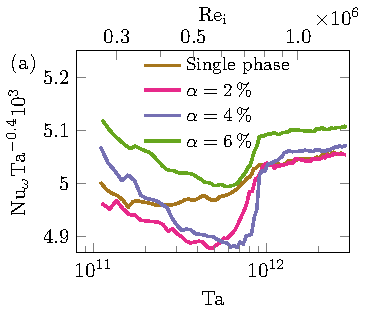
\includegraphics{figure3a.pdf}%
  \label{fig:TaNuwTaVF}
}%
\subfloat{%
    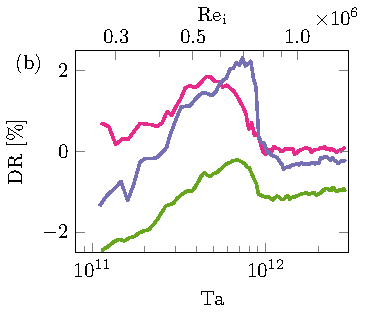
\includegraphics{figure3b.pdf}
  \label{fig:TadrVF}
}%
\caption{%
(a) $\Nus_\omega (\Tay)$, compensated by $\Tay^{0.4}$, for
\SI{8}{\milli\metre} particles with various particle volume fractions and for
comparison the single phase case.  (b) Drag reduction, defined as
$\text{DR} = \left(1 - \Nus_\omega(\alpha) / \Nus_\omega(\alpha=0) \right)$,
plotted against $\Tay$.
}
\label{fig:dragReductionVF}
\end{figure}

For a better comparison with bubbly drag reduction, we plot the drag reduction
as a function of (gas or particle) volume fraction $\alpha$; see 
\reff{fig:alphaDrAll}. Different studies are shown using different symbols, and
$\rey$ is indicated by colours. None of the datasets were compensated for the
changes in effective viscosity.   DR is defined in slightly differently
way in each study: van~den~Berg \citep{vandenBerg2005} makes use of the friction coefficient
$\left(1 - c_f(\alpha) /c_f(0) \right)$; van~Gils \citep{vanGils2013} uses the
dimensionless torque $G=\tau / (2 \pi L_{mid} \rho \nu^2)$, $\left(1 -
G(\alpha) / G(0) \right)$; and Verschoof \citep{Verschoof2016} uses the plain torque
value $\left(1 - \tau(\alpha) /\tau(0) \right)$. While the rigid particles
only showed marginal drag reduction, some studies using bubbles achieve
dramatic reduction of up to \SI{30}{\percent} and beyond. 
\refF{fig:alphaDrZoom} shows a zoomed in view of the bottom part of the plot
with the rigid sphere data. The triangles denote the data from
Verschoof \citep{Verschoof2016}, corresponding to small bubbles in the Taylor-Couette
system. The rigid particles and the small bubbles show a similar drag
response. What is remarkable is that this occurs despite the huge difference
in size. The estimated diameter of the bubbles in Verschoof \citep{Verschoof2016} is
\SI{0.1}{\milli \metre}, while the rigid spheres are about two orders in
magnitude larger. This provides key evidence that the particle size alone is
not enough to cause drag reduction, also the density ratio of the
particle and the carrier fluid is of importance.

\begin{figure}
\centering%
\subfloat{%
    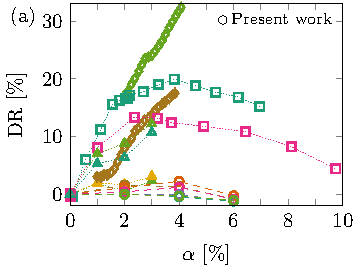
\includegraphics{figure4a.pdf}%
  \label{fig:alphaDrAll}
}%
\subfloat{%
    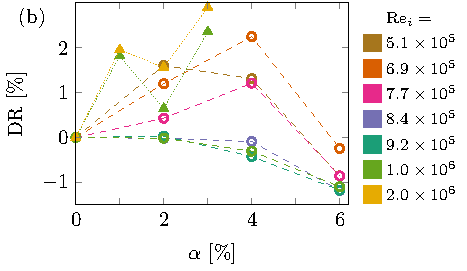
\includegraphics{figure4b.pdf}%
  \label{fig:alphaDrZoom}
}%
\caption[]{(a) Drag reduction as function of particle volume fraction from
    \marksymbol{o}{black}\,: $d_p=\SI{8}{\milli\metre}$ particles from
    present work compared to similar gas volume fractions from
    \marksymbol{square}{black}\,: van~den~Berg\citep{vandenBerg2005},
    \marksymbol{diamond}{black}\,: van~Gils\citep{vanGils2013}, and
    \marksymbol{triangle}{black}\,: Verschoof\citep{Verschoof2016}. Symbols indicate the
    different studies while colours differentiate between the Reynolds
    numbers. The current work has DR defined as $\left(1 -
        \Nus_\omega(\alpha) / \Nus_\omega(\alpha=0) \right)$; the other
        studies use dimensionless torque $G$ \citep{vanGils2013}, friction
        coefficient $c_f$ \citep{vandenBerg2005}, or plain torque $\tau$
        \citep{Verschoof2016} to define DR. (b) Zoom of the bottom part of
    (a) where the data from the present work is compared to bubbly drag
reduction data using \SI{6}{ppm} of surfactant \citep{Verschoof2016}}
\label{fig:dragReductionAlpha}
\end{figure}

\subsection{Effect of marginal changes in particle density ratio}
With the effects of particle size and volume fraction revealed, we next
address the sensitivity of the drag to marginal variations in particle
density. A change in the particle density ratio brings about a change in the
buoyancy and  centrifugal forces on the particle, both of which can affect the
particle distribution within the flow. We tune the particle to fluid density
ratio $\phi \equiv \rho_p/\rho_f$ by changing the volume fraction of glycerol
in the fluid, such that the particles are marginally buoyant ($\phi = 0.94,
0.97$), neutrally buoyant ($\phi=1.00$) and marginally heavy ($\phi=1.04$)
particles. In \reff{fig:TaNuwTaDen} we show the compensated
$\Nus_\omega$ as function of $\Tay$ for various $\phi$. $\alpha$ was fixed to
\SI{6}{\percent} and only \SI{8}{\milli\metre} particles were used. The darker
shades of colour correspond to the single phase cases, while lighter shades
correspond to particle-laden cases. In general, the single phase drag is
larger as compared to the particle-laden cases. However, there is no striking
difference between the different $\phi$.  In \reff{fig:TaDrDen}, we
present the drag reduction for particle-laden cases at different density
ratios. On average we see for all cases drag modification of approximately
$\pm$ \SI{2}{\percent}. We can also identify a small trend in the lower $\Tay$
region: the two larger $\phi$ (heavy and neutrally buoyant particles) tend to
have a drag increase, while the smaller $\phi$ cases (both light particles)
have a tendency for drag reduction. Nevertheless, the absolute difference in
DR between the cases is within 4\%. The above results provide clear evidence
that minor density mismatches do not have a serious influence on the global
drag of the system.  To investigate for strong buoyancy effects,
additional measurements were done using \SI{2}{\milli\metre} expanded
polystyrene particles ($\phi=0.02$).  However, due to the particles
accumulating between the inner cylinder segments leading to additional
mechanical friction, these measurements were inconclusive.

\begin{figure}
\centering
\subfloat{
    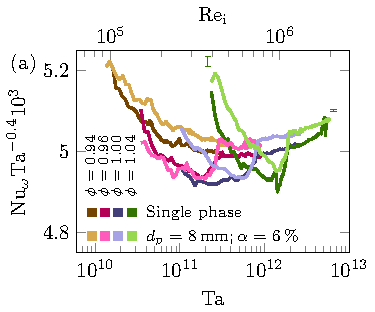
\includegraphics{figure5a.pdf}
  \label{fig:TaNuwTaDen}
}
\subfloat{
    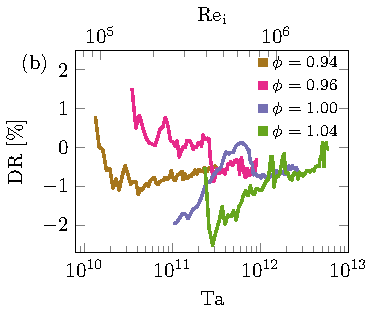
\includegraphics{figure5b.pdf}
  \label{fig:TaDrDen}
}
\caption{
(a) $\Tay$ as function of $\Nus_\omega$ compensated by $\Tay^{0.4}$ for
various density ratios $\phi=\rho_p/\rho_f$ indicated by the corresponding
colour. The darker shades indicate the single phase cases while the
lighter shades show the cases using \SI{6}{\percent} particle volume
fraction of \SI{8}{\milli\metre} diameter particles. Due to the increase
in viscosity the maximum attainable $\Tay$ is lower for larger density
ratios. The uncertainty is again estimated using the maximum
deviation from the average for multiple runs and here only shown for
the green curves. This value is slightly below \SI{1}{\percent} at
lower $\Tay$ and decreases with increasing $\Tay$ to values below
\SI{0.25}{\percent}. This trend is seen for all $\phi$.  (b) 
Drag reduction, calculated from the data of figure 5a, plotted against
$\Tay$. The drag reduction is defined as $\text{DR} = \left(1 -
\Nus_\omega(\alpha=6\%) / \Nus_\omega(\alpha=0) \right)$.
}
\label{fig:dragReductionDen}
\end{figure}
\newpage
\subsection{Flow statistics using particles} 
In the above sections, we presented the effects of changing particle size,
volume fraction, and density on the global drag of the system. Next we look
into local flow
properties using LDA while the particles are present.  First, we collected a
total of \num{1e6} data points of azimuthal velocity at mid-height and
mid-gap.  These were captured over a period of approximately $\num{3e4}$
cylinder rotations. From this data we calculate the probability density
function (PDF) of $\text{u}_\theta$ normalised by $u_i$ for various $\alpha$,
shown in \reff{fig:U_w_pdf}. The particle size was fixed to
\SI{8}{\milli\metre} and the Reynolds number was set to $\num{1e6}$. From this
figure we see a large increase in turbulent fluctuations, resulting in very
wide tails. While the difference between \SI{2}{\percent}, \SI{4}{\percent},
and \SI{6}{\percent} is not large, we can identify an increase in fluctuations
with increasing $\alpha$. These increased fluctuations can be explained by the
additional wakes produced by the particles \citep{Poelma2007,Almeras2017}. The
increase in fluctuations can also be visualized using the standard deviation
of $\sigma(u_\theta) = \left< \text{u}_\theta'^2 \right>^{1/2}$ normalised by
the standard deviation of the single phase case---see 
\reff{fig:alpha_u_rms_u0}. In this figure, $\sigma(u_\theta)$ is shown for
three different $\rey$, again for \SI{8}{\milli\metre} particles. In general,
we see a monotonically increasing trend with $\alpha$, and it seems to
approach an asymptotic value. One can speculate that there has to be an upper
limit for fluctuations which originate from wakes of the particles. For large
$\alpha$ the wakes from particles will interact with each other and with the
carried flow.

\begin{figure}
\centering%
\subfloat{%
    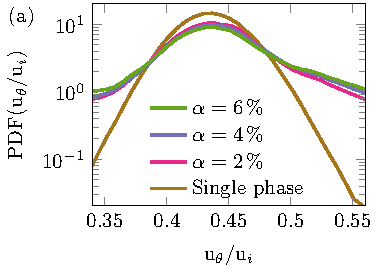
\includegraphics{figure6a.pdf}%
  \label{fig:U_w_pdf}
}%
\subfloat{%
    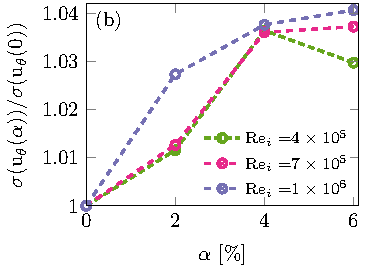
\includegraphics{figure6b.pdf}%
  \label{fig:alpha_u_rms_u0}
}%
\caption{%
(a) PDF of $\text{u}_\theta / \text{u}_i$ for various $\alpha$ and the
single phase case. The particle size was fixed to \SI{8}{\milli\metre}
and $\rey_i=\num{1e6}$ for all cases. (b) Standard deviation of the
azimuthal velocity normalized by the standard deviation of the single phase
case for three different $\rey$ for a fixed particle size of
\SI{8}{\milli\metre}.} \label{fig:ldaresults}
\end{figure}

Measurements using \SI{4}{\milli\metre} particles yielded qualitatively
similar results. It is known that in particle-laden gaseous pipe flows, large
particles can increase the turbulent fluctuations, while small particles
result in turbulence attenuation \citep{Tsuji1984,Gore1989,Vreman2015}. The
LDA measurements were not possible with the smallest particles
(\SI{1.5}{\milli\metre}), as the large amount of particles in the flow blocked
the optical paths of the laser beams.

We are confident that for these bi-disperse particle-laden LDA measurements,
the large particles do not have an influence on the measurements as these
\emph{millimetric}-sized particles are much larger than the fringe spacing
($d_f = \SI{3.4}{\micro\metre}$) and do not show a Doppler burst.  However,
during the measurements the particles get damaged and small bits of material
are fragmented off the particles. We estimate the size of these particles
slightly larger than the tracer particles and these can have an influence on
the LDA measurements as they do not act as tracers.

How the average azimuthal velocity changes with particle radius is shown in
\reff{fig:ldaradial}.  We measured a total of $\num{3e4}$ data points
during approximately 900 cylinder rotations. Again, the data were corrected
for velocity bias by using the transit time as a weighing factor. 
\refF{fig:U_theta_radius_size} shows the effect of particle size for
$\alpha=\SI{2}{\percent}$, and \reff{fig:U_theta_radius_vol} shows the
effect of particle volume fraction for \SI{8}{\milli\metre} particles. Both
figures additionally show the high-precision single phase data from another
study \citep{Huisman2013} for which our single phase measurements are practically
overlapping. Since LDA measurements close to the inner cylinder are difficult,
due to the reflecting inner cylinder surface, we limited our radial extent to
$\tilde{r}=(r - r_i) / (r_o - r_i)=[0.2,1]$. We found that the penetration
depth of our LDA measurements is the smallest for experiments with the
smallest particles and the largest $\alpha$. All differences with the single
phase case are only marginal and we can conclude that the average mean
velocity is not much affected by the particles in the flow, at least for
$\tilde{r} \geq 0.2$.

\begin{figure}
\centering%
\subfloat{%
    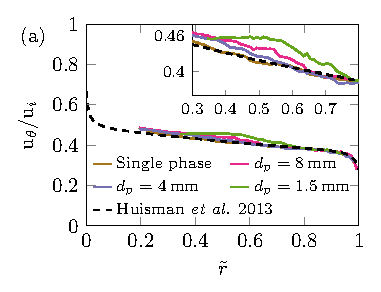
\includegraphics{figure7a.pdf}%
  \label{fig:U_theta_radius_size}
}%
\subfloat{%
    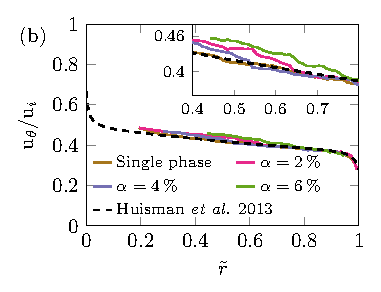
\includegraphics{figure7b.pdf}%
  \label{fig:U_theta_radius_vol}
}%
\caption{%
$\text{u}_\theta$ normalised by the velocity of the inner cylinder wall
$\text{u}_i$ as function of the normalised radius for various $d_p$ while
$\alpha=\SI{2}{\percent}$ (a) and various $\alpha$ while
$d_p=\SI{8}{\milli\metre}$ (b). In all cases $\rey_i$ is fixed to $\num{1e6}$.
For comparison, the single phase case using water at $\rey_i=\num{1e6}$ from
Huisman~\citep{Huisman2013} is also plotted in dashed black in both plots. Both figures
have an inset showing an enlargement of the centre area from the same
figure.} \label{fig:ldaradial}
\end{figure}

\begin{figure}
\centering%
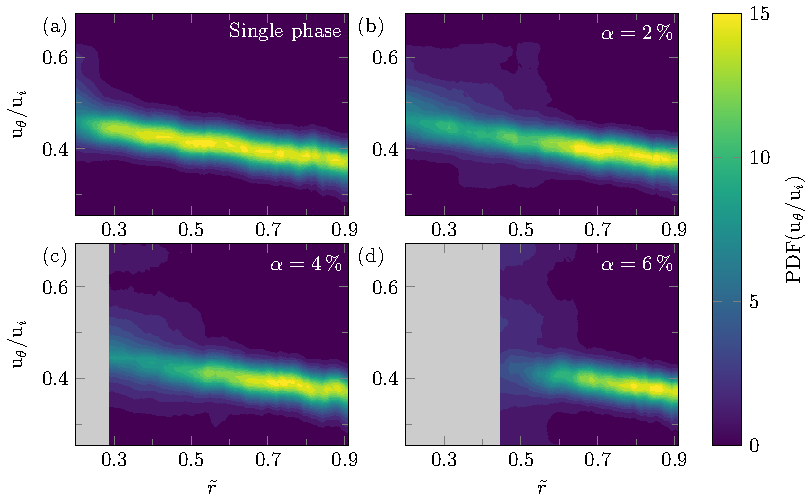
\includegraphics{figure8.pdf}%
\caption{%
\label{fig:heatmap}
PDF of the normalised azimuthal velocity as a function of normalised radial
position for various $\alpha$ for the case of \SI{8}{\milli\metre} particles
and the single phase case while keeping $\rey$ at $\num{1e6}$. With increasing
$\alpha$ the maximum penetration depth decreases. The grey areas indicate
radial positions for which no data is available.
}
\end{figure}

To get an idea of the fluctuations we can use the previous data to construct a
two-dimensional PDF of the azimuthal velocity as function of radius. These are
shown for $\rey = \num{1e6}$ using \SI{8}{\milli\metre} particles at various
$\alpha$ and the single phase case in \reff{fig:heatmap}.  First thing
to notice is again that the penetration depth is decreasing with increasing
$\alpha$.  The single phase case shows a narrow banded PDF. When $\alpha$ is
increased, for the lower values of $\tilde{r}$ the PDF is much wider.  While
it makes sense that an increase in $\alpha$ increases the fluctuations due to
the increased number of wakes of particles, this is expected everywhere in the
flow, not only closer to the inner cylinder.  It is possible that the
particles have a preferred concentration closer to the inner cylinder.  We
have tried to measure the local concentration of particles as function of
radius but failed due to limited optical accessibility.  Therefore, we can
only speculate under what circumstances there would be an inhomogeneous
particle distribution which would lead to the visible increase in
fluctuations.  The first possibility is a mismatch in density between the
particle and the fluid, which would result in light particles ($\phi < 1$) to
accumulate closer to the inner cylinder.  Another possibility is that due to
the rotation of the particle, an effective lift force arises, leading to a
different particle distribution in the flow. While this is quite plausible,
this is difficult to validate as we would need to capture the rotation.  The
fragments of plastic that are sheared off the particles can also have a bias
to the LDA measurement. While we estimate them to be larger than the tracers,
they might still be small enough to produce a signal and they might not follow
the flow faithfully.

\section{Conclusions and outlook}\label{sec:conclusions_and_outlook}
We have conducted an experimental study on the drag response of a highly
turbulent Taylor-Couette flow containing rigid neutrally buoyant spherical
particles. We have found that, unlike the case of bubbles used in prior
works~\citep{vanGils2013,Verschoof2016}, rigid particles barely reduce (or
increase) the drag on the system, even for cases where their size was
comparable to that of bubbles used in other studies.
There was no significant size effect. Even for very large particles, which can
attenuate turbulent fluctuations and generate wakes, there was no distinct
difference with the single phase flow.
We also varied the volume fraction of the particles in the range 0\%--6\%. The
particle volume fraction has no greater effect on the system drag than what is
expected due to changes in the apparent viscosity of the suspension. Further,
we tested the sensitivity of our drag measurements to marginal variations in
particle to fluid density ratio $\phi$. A trend was noticeable, towards drag
reduction when $\phi$ was reduced from 1.00 to 0.94. This suggests that a low
density of the particle could be a necessary ingredient for drag reduction.
Finally, we have also probed the local flow at the mid height and mid gap of
the system using LDA. With the addition of particles, the liquid velocity
fluctuations are enhanced, with wider tails of the distributions. A finite
relative velocity between the particle and the flow around it can cause this
increase in velocity fluctuations~\citep{Mathai2015}, as seen for bubbly flows
(pseudo-turbulence), and in situations of sedimenting particles in quiescent
or turbulent environments~\citep{Gore1989}.  In the present situation, the
relative velocity between the particle and the flow is expected, owing to the
inertia of the finite-sized particles we used.
There is only a marginal deviation from the single phase case in the average
azimuthal velocity over the radial positions measured using any size or
concentration of particles measured. From the two-dimensional PDFs, we see
that closer to the inner cylinder, using smaller $d_p$ or larger $\alpha$, the
PDF gets wider. This can be due to a preferential concentration of the
particles or a slight density mismatch.

\textcolor{black}{Our study is a step towards a better understanding of the
mechanisms of bubbly drag reduction. Bubbles are deformable, and they have
a tendency to migrate towards the walls, either due to lift
force~\citep{Dabiri2013}, or due to the centripetal
effects~\citep{vanGils2013}. When compared to the drag reducing bubbles 
\citep{vanGils2013,Verschoof2016}, our particles do not deform, and they do
not experience centripetal effects as they are density matched.  At
least one of these differences must therefore be crucial for the observed,
bubbly drag reduction in those experiments.
In a future investigation, we will conduct more experiments using very light
spherical particles that experience similar centripetal forces as the bubbles
in van~Gils~\citep{vanGils2013}, but are non-deformable.} These particle need to be
larger than the size of the gap between the inner cylinder segments and very
rigid, or the setup needs to be modified to close the gap between the IC
segments.  Such experiments can then disentangle the role of particle density
on drag reduction from that of the particle shape.

\graphicspath{{fig/}}

   % Fibers
%%%%%%%%%%%%%%%%%%%%%%%%%%%
%%% Chapter definitions %%%
%%%%%%%%%%%%%%%%%%%%%%%%%%%
% Chapter title
\renewcommand{\mychaptertitle}{%
Finite-sized rigid spheres in turbulent Taylor-Couette flow: %
Effect on the overall drag%
}
% Chapter short title
\renewcommand{\mychaptershorttitle}{%
Finite-sized rigid spheres in turbulent Taylor-Couette flow%
}
% Chapter authors
\renewcommand{\mychapterauthors}{%
\textbf{Dennis~Bakhuis},
Ruben~A.~Verschoof,
Varghese~Mathai,
Sander~G.~Huisman,
Detlef~Lohse,
and
Chao~Sun
\textit{Finite-sized rigid spheres in turbulent Taylor-Couette flow:
Effect on the overall drag},
J. Fluid Mech. \textbf{850}, 246--261 (2018).
}
% Chapter abstract
\renewcommand{\mychapterabstract}{%
We report on the modification of drag by neutrally buoyant spherical
finite-sized particles in highly turbulent Taylor-Couette (TC) flow.  These
particles are used to disentangle the effects of size, deformability, and
volume fraction on the drag, and are contrasted with the drag in bubbly TC
flow.  From global torque measurements we find that rigid spheres hardly
decrease or increase the torque needed to drive the system.   The size of the
particles under investigation have a marginal effect on the drag, with smaller
diameter particles showing only slightly lower drag.  Increasing the particle
volume fraction shows a net drag increase, however this increase is much
smaller than can be explained by the increase in apparent viscosity due to the
particles.  The increase in drag for increasing particle volume fraction is
corroborated by performing laser Doppler anemometry where we find that the
turbulent velocity fluctuations also increase with increasing volume fraction.
In contrast with rigid spheres, for bubbles the effective drag reduction also
increases with increasing Reynolds number. Bubbles are also much more
effective in reducing the overall drag. 
}
\renewcommand{\mychaptermark}{Neutrally buoyant spheres}
\renewcommand{\mychapterlabel}{chap:spheres}
\renewcommand{\mychaptericon}{fig/swchapter1.png}
%%%%%%%%%%%%%%%%%%%%%%%%%%%%%
%%% Create Chapter Header %%%
%%%%%%%%%%%%%%%%%%%%%%%%%%%%%
%%%%%%%%%%%%%%%%%%%%%%
%%% Chapter header %%%
%%%%%%%%%%%%%%%%%%%%%%
\globalcolor{ChapterText}
\chapter[\mychaptershorttitle]{%
    \mychaptertitle%
    \ifdefined\starwarsfootnotes
        \textsuperscript{%
            \hspace{-1mm}%
            \includegraphics[height=\swsymsize]{\mychaptericon}%
        }%
        \blfootnote{%
            \textcolor{footnotetextcolor}{%
                \textsf{%
                    \vspace{0.5mm}\hspace{-1mm}%
                    \includegraphics[height=\swfnsymsize]{\mychaptericon}%
                    \hspace{0.5mm}%
                    Based on: \mychapterauthors%
                }
            }
        }
    \else
        \footnote{\textsf{%
             Based on: \mychapterauthors%
        }}%
    \fi
}
\pagecolor{ChapterBackground}
\afterpage{\pagecolor{White}\globalcolor{Black}} 
\label{\mychapterlabel}
\chaptermark{\mychaptermark}
\noindent\rule{\textwidth}{0.4pt}%
\vspace{0.2cm}
\noindent\textsf{\mychapterabstract}
\clearpage

%%%%%%%%%%%%%%%%%%%%%%%%
%%%% end title page %%%%
%%%%%%%%%%%%%%%%%%%%%%%%
\graphicspath{{ChapterOne/fig/}}
\section{Introduction}
Flows in nature and industry are generally turbulent, and often these flows
carry bubbles, drops, or particles of various shapes, sizes, and densities.
Examples include sediment-laden rivers, gas-liquid reactors, volcanic
eruptions, plankton in the oceans, pollutants in the atmosphere, and air
bubbles in the ocean mixing layer~\citep{Toschi2009}.  Particle-laden flows
may be characterized in terms of particle density $\rho_p$, particle diameter
$d_p$, volume fraction $\alpha$, and Reynolds number Re of the flow. When
$d_p$ is small (compared to the dissipative length scale $\eta_K$) and
$\alpha$ low ($< 10^{-3}$), the system may be modelled using a point particle
approximation with two-way
coupling~\citep{Elghobashi1994,Mazzitelli2003,Mathai2016}.  With recent
advances in computing, fully resolved simulations of particle-laden flows have
also become feasible.  Uhlmann conducted one of the first numerical
simulations of finite-sized rigid spheres in a vertical particle-laden channel
flow \citep{Uhlmann2008}.  They observed a modification of the mean velocity
profile and turbulence modulation due to the presence of particles. A number
of studies followed, which employed immersed
boundary~\citep{Peskin2002,Cisse2013}, Physalis~\citep{Naso2010, Wang2017b},
and front-tracking methods~\citep{Unverdi1992,Roghair2011,Tagawa2013} to treat
rigid particles and deformable bubbles, respectively, in channel and pipe flow
geometries~\citep{Pan1996,Lu2005,Uhlmann2008,Dabiri2013,Kidanemariam2013,Lashgari2014,Picano2015,Costa2016}. 
Flows with dispersed particles, drops, and bubbles can, under the right
conditions, reduce skin friction and result in significant energetic (and
therefore financial) savings. In industrial settings this is already achieved
using polymeric additives which disrupt the self-sustaining cycle of wall
turbulence and dampen the quasi-streamwise vortices
\citep{White2008,Procaccia2008}. Polymeric additives are impractical for
maritime applications, and therefore gas bubbles are used with varying success
rates \citep{Ceccio2010,Murai2014}. Local measurements in bubbly flows are
non-trivial and the key parameters and their optimum values are still unknown.
For example, it is impossible to fix the bubble size in experiments and
therefore to isolate the effect of bubble size. Various studies hinted that
drag reduction can also be achieved using spherical particles
\citep{Zhao2010}, also by using very large particles in a turbulent von
K\'arm\'an flow \citep{Cisse2015}. In this latter study a tremendous decrease
in turbulent kinetic energy (TKE) was observed. A similar, but less intense,
decrease in TKE was also seen using a very low particle volume
fraction\citep{Bellani2012b}. By using solid particles it is possible to
isolate the size effect on drag reduction and even though rigid particles are
fundamentally different from bubbles, this can give additional insight into
the mechanism of bubbly drag reduction.  The particle dynamics are highly
influenced by the diameter of the particle\citep{Machicoane2016}. This might
or might not have a direct influence on the global drag of the system and has
never been studied.
%
Whether and when solid particles increase or decrease the drag in a flow is
yet not fully understood and two lines of thought exist. On one side, it is
hypothesized that solid particles {\it decrease} the overall drag as they damp
turbulent fluctuations \citep{Zhao2010,Poelma2007}. On the other side, one
could expect that solid particles {\it increase} drag as they shed vortices,
which must be dissipated. In addition, they also increase the apparent
viscosity. A common way to quantify this is the so called `Einstein
relation'~\citep{Einstein1906}
\begin{equation} \nu_\alpha = \nu\left(1 +
\frac{5}{2}\alpha \right), \label{eq:einstein} \end{equation} where $\nu$ is
the viscosity of the continuous phase. This compensation is valid for the
small $\alpha$ values used in this \docname \citep{Stickel2005}. Direct
measurements of drag in flows with solid particles are scarce, and the debate
on under what condition they either enhance or decrease the friction has not
yet been settled. Particles and bubbles may show collective effects
(clustering) and experiments have revealed that this has significant influence
on the flow properties~\citep{Liu1993, Kulick1994, Muste1997, So2002,
Fujiwara2004, vandenBerg2005, vandenBerg2007, Shawkat2008, Calzavarini2008,
Colin2012, vanGils2013, Maryami2014, Mathai2015,
Almeras2017,Mathai2018}. In general, the Stokes number is used to
predict this clustering behaviour, but for neutrally buoyant particles this is
found to be insufficient \citep{Bragg2015,Fiabane2012}. In addition, the
position of the particles (or the particles clusters) is likely to have a
large influence on the skin friction.  It was shown in DNS at low Reynolds
numbers, that the particle distribution is mainly
governed by the bulk Reynolds number\citep{Kazerooni2017}.

In order to study the effects of particles on turbulence it is convenient to
use a closed setup where one can relate global and local quantities directly
through rigorous mathematical relations. In this \docname the Taylor-Couette
(TC) geometry~\citep{Grossmann2016}---the flow between two concentric rotating
cylinders---is employed as this is a closed setup with global balances. The
driving of the Taylor-Couette geometry can be described using the Reynolds
number based on the inner cylinder (IC): $\rey_i = u_i d / \nu$, where $u_i =
\omega_i r_i$ is the azimuthal velocity at the surface of the IC, $\omega_i$
the angular velocity of the IC, $d = r_o - r_i$ the gap between the cylinders,
$\nu$ the kinematic viscosity, and $r_i$($r_o$) the radius of the inner(outer)
cylinder. The geometry of Taylor-Couette flow is characterized by two
parameters: the radius ratio $\eta=r_i/r_o$ and the aspect ratio $\Gamma =
L/d$, where $L$ is the height of the cylinders. The response parameter of the
system is the torque, $\tau$, required to maintain constant rotation speed of
the inner cylinder. It was mathematically shown that in Taylor-Couette flow
the angular velocity flux defined as $J^\omega = r^3 \left(  \left
\langle u_r \omega \right \rangle_{A,t} - \nu \frac{\partial} {\partial r}
\left \langle \omega \right \rangle_{A,t} \right)$, where the subscript $A,t$
denotes averaging over a cylindrical surface and time,	is a radially
conserved quantity (Eckhardt, Grossmann, Lohse \citep{Eckhardt2007} (EGL)). One can, in analogy to
Rayleigh-B\'enard convection, normalize this flux and define a Nusselt number
based on the flux of the angular velocity:
\begin{equation}
  \Nus_\omega = \frac{J^\omega}{J^\omega_{\text{lam}}} = \frac{\tau}{2 \pi L \rho J^\omega_{\text{lam}}},
\end{equation}
where $J^\omega_{\text{lam}} = 2 \nu r^2_i r^2_o \left( \omega_i - \omega_o
\right)/\left( r^2_o - r^2_i \right)$ is the angular velocity flux for
laminar, purely azimuthal flow and $\omega_o$ is the angular velocity of the
outer cylinder. In this spirit the driving is expressed in terms of the Taylor
number:
\begin{equation}
  \Tay = \frac{1}{4} \sigma d^2 \left(r_i + r_o \right)^2 \left( \omega_i - \omega_o \right)^2 \nu^{-2}.
\end{equation}
Here $\sigma = \left( \left( 1 + \eta \right) / \left(2 \sqrt{\eta} \right)
\right)^4\;\approx\;1.057$ is a geometric parameter (``geometric Prandtl
number''), in analogy to the Prandtl number in Rayleigh-B\'enard convection.
In the presented work, where only the inner cylinder is rotated and the outer
cylinder is kept stationary, we can relate $\Tay$ to the Reynolds number of
the inner cylinder by
\begin{equation}
\rey_i = \frac{r_i \omega_i d}{\nu} = \frac{8\eta^2}{(1+\eta)^{3}} \sqrt{\Tay}.
\end{equation}
\noindent The scaling of the dimensionless angular velocity flux (torque) with
the Taylor (Reynolds) number has been analysed extensively, see e.g.
\citep{Lathrop1992,Lewis1999,Paoletti2011,vanGils2011,Ostilla-Monico2013} and
the review articles \citep{Fardin2014,Grossmann2016}, and the
different regimes are well understood. In the current Taylor number regime it
is known that $\Nus_\omega \propto \Tay^{0.4}$. Because this response is
well known, it can be exploited to study the influence of immersed bubbles and
particles
~\citep{vandenBerg2005,vandenBerg2007,vanGils2013,Maryami2014,Verschoof2016}
on the drag needed to sustain constant rotational velocity of the inner
cylinder. 

In this \docname we will use the TC geometry to study the effect of neutrally
buoyant rigid spherical particles on the drag. We study the effects of varying
the particle size $d_p$, the volume fraction $\alpha$, the density ratio
$\phi$, and the flow Reynolds number $\text{Re}$ on the global torque (drag)
of the Taylor-Couette flow. The drag reduction is expressed as $\text{DR} =
\left(1 - \Nus_\omega(\alpha) / \Nus_\omega(\alpha=0) \right)$ and as we are
interested in the net drag reduction, it is \emph{not} compensated for
increased viscosity effects using correction models, such as the Einstein
relation.

The \docname is organized as follows. \refSec{sec:experimentalSetup}
presents the experimental setup. In \refsec{sec:sphereresults} we discuss the
results. The findings are summarized and an outlook for future work is given
in the last section.

\section{Experimental setup}\label{sec:experimentalSetup}
The experiments were conducted in the Twente Turbulent Taylor-Couette
(T${}^3$C) facility \citep{vanGils2011}. A schematic of the setup is shown in
\reff{fig:setup}. In this setup, the flow is confined between two
concentric cylinders, which rotate independently. The top and bottom plates
are attached to the outer cylinder. The radius of the inner cylinder (IC) is
$r_i = \SI{0.200}{\metre}$ and the radius of the outer cylinder (OC) is $r_o =
\SI{0.2794}{\metre}$, resulting in a gap width of $d = r_o - r_i =
\SI{0.0794}{\metre}$ and a radius ratio of $\eta = r_i/r_o = 0.716$. The IC
has a total height of $L = \SI{0.927}{\metre}$ resulting in an aspect ratio of
$L / d = 11.7$. The IC is segmented axially in three parts. To minimize the
effect of the stationary end plates, the torque is measured only over the
middle section of the IC with height $L_{\text{mid}}/L = 0.58$, away from
the end plates. A hollow reaction torque sensor made by Honeywell is used to
measure the torque which has an error of roughly 1\% for the largest torques
we measured. Between the middle section and the top and bottom section of the
inner cylinder is a gap of 2mm.

The IC can be rotated up to $f_i = \omega_i/(2\pi) =
\SI{20}{\hertz}$. In these experiments only the IC is rotated and the OC is
kept at rest. The system holds a volume of $V = \SI{111}{\litre}$ of working
fluid, which is a solution of glycerol ($\rho =
\SI{1260}{\kilo\gram/\metre\cubed}$) and water. To tune the density of the
working fluid, the amount of glycerol was varied between \SI{0}{\percent} and
\SI{40}{\percent} resulting in particles being marginally heavy,
neutrally buoyant, or marginally light.
\begin{figure}
\centering
\includegraphics[height=5.5cm]{figure1.pdf}
\caption{
Schematic of the Taylor-Couette setup. Two concentric cylinders of radii
$r_{i,o}$ with a working fluid in between. Particles are not to scale. The
inner cylinder rotates with angular velocity $\omega_i$, while the outer
cylinder is kept at rest. We measure the torque on the middle section
(highlighted). The laser Doppler anemometry (LDA) probe is positioned at mid
height to measure the azimuthal velocity at mid gap.}
\label{fig:setup}
\end{figure}
The system is thermally controlled by cooling the top and bottom plates of the
setup. The temperature was kept at $T = \SI{20(1)}{\celsius}$ for all the
experiments, with a maximum spatial temperature difference of
$\SI{0.2}{\kelvin}$ within the setup, and we account for the density and
viscosity changes of water and glycerol \citep{Glycerine1963}.

Rigid polystyrene spherical particles (\textit{RGPballs S.r.l.}) were used in
the experiments, these particles have a density close to that of water
(940\,--\SI{1040}{\kilo\gram/\metre\cubed}). We chose particles with diameters
$d_p = 1.5$, 4.0, and $\SI{8.0}{\milli\metre}$. To our disposal are:
\SI{2.22}{\litre} of \SI{1.5}{\milli\metre} diameter particles,
\SI{2.22}{\litre} of \SI{4}{\milli\metre} diameter particles, and
\SI{6.66}{\litre} of \SI{8}{\milli\metre} diameter particles, resulting in
maximum volume fractions of \SI{2}{\percent}, \SI{2}{\percent}, and
\SI{6}{\percent}, respectively. The particles are found to be nearly
mono-disperse (\SI{99.9}{\percent} of the particles are within \SI{\pm
0.1}{\milli\metre} of their target diameter). Due to the fabrication process,
small air bubbles are sometimes entrapped within the particles. This results
in a slight heterogeneous density distribution of the particles. After
measuring the density distribution for each diameter, we calculated the
average for all batches, which is $\rho_p = \SI{1036 \pm
5}{\kilo\gram/\metre\cubed}$. By adding glycerol to water we match this value
in order to have neutrally buoyant particles.

Using a laser Doppler anemometry (LDA) system (BSA F80, Dantec Dynamics) we
captured the azimuthal velocity at mid-height and mid-gap of the system (see
\reff{fig:setup}) and we performed a radial scan at mid-height.
The flow was seeded with \SI{5}{\micro\metre} diameter polyamide particles
(PSP-5, Dantec Dynamics). Because of the curved surface of the outer cylinder
(OC), the beams of the LDA get refracted in a non-trivial manner, which was
corrected for using a ray-tracing technique \citep{Huisman2012}. 

Obviously, LDA measurements in a multi-phase flow are more difficult to set up
than for single phase flows, as the method relies on the reflection of
light from tiny tracer particles passing through a measurement volume
($\SI{0.07}{\milli\metre} \times \SI{0.07}{\milli\metre} \times
\SI{0.3}{\milli\metre}$).  Once we add a second type of relatively large
particles to the flow, this will affect the LDA measurements, mostly by
blocking the optical path, resulting in lower acquisition rates. These large
particles will also move through the measurement volume, but as these
particles are at least 300 times larger than the tracers and thus much larger
than the fringe pattern (fringe spacing $d_f=\SI{3.4}{\micro\metre}$), the
reflected light is substantially different from a \emph{regular} Doppler burst
and does not result in a measured value. The minimal signal-to-noise ratio for
accepting a Doppler burst was set to 4. As a post-processing step the
velocities were corrected for the velocity bias by using the transit time of
the tracer particle.
\newpage
\section{Results}\label{sec:sphereresults}
\subsection{Effect of particle size}\label{subsec:sizeEffect}
First we study the effect of changing the particle diameter on the torque of
the system. In these experiments, we kept the particle volume fraction fixed
at \SI{2}{\percent} and the density of the working fluid, $\rho_f$, at
\SI{1036}{\kilogram/\metre \cubed}, for which the particles are neutrally
buoyant. The results of these measurements are presented as
$\Nus_\omega(\Tay)$ in \reff{fig:TaNuwSize}. Our curves are practically
overlapping, suggesting that the difference in drag between the different
particle sizes is only marginal. We compare these with the bubbly drag
reduction data at similar conditions (hollow symbols) 
\citep{Verschoof2016,vanGils2013,vandenBerg2005}. At low $\Tay$ the symbols
overlap with our data. However, at larger $\Tay$, the bubbly flow data shows
much lower torque (drag) than the particle-laden cases. As we are in the
ultimate regime of turbulence where $\Nus_\omega$ effectively scales as
$\Nus_\omega \propto \Tay^{0.4}$~\citep{Huisman2012,Ostilla-Monico2013}, we
compensate the data with $\Tay^{0.40}$ in \reff{fig:TaNuwTaSize} to
emphasize the differences between the datasets. For the single phase
case, this yields a clear plateau. For the particle-laden cases, the lowest
drag corresponds to the smallest particle size. The reduction is however quite
small ($<\SI{3}{\percent}$). The compensated plots also reveal a sudden
increase in drag at a critical Taylor number $\Tay^* =\num{0.8e12}$. The jump
is more distinct for the smaller particles, and might suggest a reorganisation
of the flow \citep{Huisman2014}. Beyond $\Tay^*$, the drag reduction is
negligible for the larger particles (\SI{4}{\milli \metre} and \SI{8}{\milli
\metre} spheres). However, for the \SI{1.5}{\milli\metre} particles, the drag
reduction seems to increase, and was found to be very repeatable in
experiments. Interestingly, the size of these particles is comparable to that
of the air bubbles \citep{vanGils2013}.  This might suggest that for smaller
size particles at larger $\Tay$, one could expect drag reduction. At the
increased viscosity of the suspension, a maximum $\Tay \approx 3 \times
10^{12}$ could be reached in our experiments.   We have performed an
uncertainty analysis by repeating the measurements for the single phase, and
for the cases with \SI{8}{\milli\metre} and \SI{1.5}{\milli\metre} particles
multiple times and calculating the maximum deviation from the ensemble
average.  The left error bar indicates the maximum deviation for all
measurements combined and is $\approx \SI{1}{\percent}$.  For $\Tay \geq
\num{2e12}$, we see an increase in uncertainty of \SI{1.7}{\percent} (shown by
the right error bar in \reff{fig:TaNuwTaSize}), which is only caused by
the \SI{1.5}{\milli\metre} particles. These tiny particles can accumulate in
the \SI{2}{\milli\metre} gap between the cylinder segments and thereby
increase the uncertainty. Above $\Tay \geq \num{2e12}$, both, the
\SI{8}{\milli\metre} and \SI{4}{\milli\metre} particles, show a maximum
deviation below 0.25\%.\\
%
\begin{figure}
\centering%
\subfloat{%
    \includegraphics{figure2a.pdf}%
  \label{fig:TaNuwSize}
}%
\subfloat{%
    \includegraphics{figure2b.pdf}
  \label{fig:TaNuwTaSize}
}%
\caption{%
(a) $\Nus_\omega (\Tay)$ for \SI{2}{\percent} particle volume fraction with
particle diameters of \SI{1.5}{\milli\metre}, \SI{4.0}{\milli\metre}, and
\SI{8.0}{\milli\metre}, and for comparison the single phase case. Data from
comparable bubbly drag reduction studies are plotted using black markers. (b)
Same data, but now as compensated plot $\Nus_\omega / \Tay^{0.40}$ as function
of $\Tay$.   The error bar indicates the maximum deviation for repeated
measurements from all measurements combined (coloured curves) which is less
than \SI{1}{\percent}. At $\Tay \geq \num{2e12}$, the \SI{1.5}{\milli\metre}
particles show an increased uncertainty of \SI{1.7}{\percent}, which is
indicated by the right error bar.}
\label{fig:dragReductionSize}
\end{figure}
%
\indent Below $\Tay^*$, the drag reduction due to spherical particles appears to be
similar to bubbly drag reduction~\citep{vanGils2013}. However, in the lower
$\Tay$ regime, the bubble distribution was highly non-uniform due to buoyancy
of the bubbles~\citep{vandenBerg2005,vanGils2013,Verschoof2016}. Therefore,
the volume fractions reported were only the global values, and the torque
measurements were for the mid-sections of their setups. What is evident from
the above comparisons is that in the high $\Tay$ regime, air bubbles
drastically reduce the drag, reaching far beyond the drag modification by
rigid spheres.
\newpage
\subsection{Effect of particle volume fraction}\label{subsec:volumeFraction}
The next step is to investigate the effect of the particle volume fraction on
the torque. For the \SI{8}{\milli\metre} particles, we have the ability to
increase the particle volume fraction up to \SI{6}{\percent}. This was done in
steps of \SI{2}{\percent}, and the results are plotted in compensated form in
\reff{fig:TaNuwTaVF}. The normalised torque increases with the volume
fraction of particles. The \SI{6}{\percent} case shows the largest drag.
\refF{fig:TadrVF} shows the same data in terms of drag reduction as
function of $\Tay$. A \SI{2}{\percent} volume fraction of particles gives the
highest drag reduction. With increasing $\alpha$ the drag reduction decreases.
These measurements are in contrast with the findings for bubbly drag
reduction~\citep{vanGils2013}, for which the net drag decreases with
increasing gas volume fraction.
of drag in a particle-laden flow is the larger apparent viscosity.  If we
would calculate the apparent viscosity for our case with the Einstein relation
(\refe{eq:einstein}) for $\alpha=\SI{6}{\percent}$, the drag increase
would be \SI{15}{\percent}, as compared to the pure working fluid.  Including
this effect in our drag reduction calculation would result in reductions of
the same order.  However, when comparing the drag with or without particles,
the \emph{net} drag reduction is practically zero. This result is different
from the work a in turbulent channel flow where they found
that the drag increased more than the increase of the viscosity\citep{Picano2015}.

\begin{figure}
\centering%
\subfloat{%
    \includegraphics{figure3a.pdf}%
  \label{fig:TaNuwTaVF}
}%
\subfloat{%
    \includegraphics{figure3b.pdf}
  \label{fig:TadrVF}
}%
\caption{%
(a) $\Nus_\omega (\Tay)$, compensated by $\Tay^{0.4}$, for
\SI{8}{\milli\metre} particles with various particle volume fractions and for
comparison the single phase case.  (b) Drag reduction, defined as
$\text{DR} = \left(1 - \Nus_\omega(\alpha) / \Nus_\omega(\alpha=0) \right)$,
plotted against $\Tay$.
}
\label{fig:dragReductionVF}
\end{figure}

For a better comparison with bubbly drag reduction, we plot the drag reduction
as a function of (gas or particle) volume fraction $\alpha$; see 
\reff{fig:alphaDrAll}. Different studies are shown using different symbols, and
$\rey$ is indicated by colours. None of the datasets were compensated for the
changes in effective viscosity.   DR is defined in slightly differently
way in each study: van~den~Berg \citep{vandenBerg2005} makes use of the friction coefficient
$\left(1 - c_f(\alpha) /c_f(0) \right)$; van~Gils \citep{vanGils2013} uses the
dimensionless torque $G=\tau / (2 \pi L_{mid} \rho \nu^2)$, $\left(1 -
G(\alpha) / G(0) \right)$; and Verschoof \citep{Verschoof2016} uses the plain torque
value $\left(1 - \tau(\alpha) /\tau(0) \right)$. While the rigid particles
only showed marginal drag reduction, some studies using bubbles achieve
dramatic reduction of up to \SI{30}{\percent} and beyond. 
\refF{fig:alphaDrZoom} shows a zoomed in view of the bottom part of the plot
with the rigid sphere data. The triangles denote the data from
Verschoof \citep{Verschoof2016}, corresponding to small bubbles in the Taylor-Couette
system. The rigid particles and the small bubbles show a similar drag
response. What is remarkable is that this occurs despite the huge difference
in size. The estimated diameter of the bubbles in Verschoof \citep{Verschoof2016} is
\SI{0.1}{\milli \metre}, while the rigid spheres are about two orders in
magnitude larger. This provides key evidence that the particle size alone is
not enough to cause drag reduction, also the density ratio of the
particle and the carrier fluid is of importance.

\begin{figure}
\centering%
\subfloat{%
    \includegraphics{figure4a.pdf}%
  \label{fig:alphaDrAll}
}%
\subfloat{%
    \includegraphics{figure4b.pdf}%
  \label{fig:alphaDrZoom}
}%
\caption[]{(a) Drag reduction as function of particle volume fraction from
    \marksymbol{o}{black}\,: $d_p=\SI{8}{\milli\metre}$ particles from
    present work compared to similar gas volume fractions from
    \marksymbol{square}{black}\,: van~den~Berg\citep{vandenBerg2005},
    \marksymbol{diamond}{black}\,: van~Gils\citep{vanGils2013}, and
    \marksymbol{triangle}{black}\,: Verschoof\citep{Verschoof2016}. Symbols indicate the
    different studies while colours differentiate between the Reynolds
    numbers. The current work has DR defined as $\left(1 -
        \Nus_\omega(\alpha) / \Nus_\omega(\alpha=0) \right)$; the other
        studies use dimensionless torque $G$ \citep{vanGils2013}, friction
        coefficient $c_f$ \citep{vandenBerg2005}, or plain torque $\tau$
        \citep{Verschoof2016} to define DR. (b) Zoom of the bottom part of
    (a) where the data from the present work is compared to bubbly drag
reduction data using \SI{6}{ppm} of surfactant \citep{Verschoof2016}}
\label{fig:dragReductionAlpha}
\end{figure}

\subsection{Effect of marginal changes in particle density ratio}
With the effects of particle size and volume fraction revealed, we next
address the sensitivity of the drag to marginal variations in particle
density. A change in the particle density ratio brings about a change in the
buoyancy and  centrifugal forces on the particle, both of which can affect the
particle distribution within the flow. We tune the particle to fluid density
ratio $\phi \equiv \rho_p/\rho_f$ by changing the volume fraction of glycerol
in the fluid, such that the particles are marginally buoyant ($\phi = 0.94,
0.97$), neutrally buoyant ($\phi=1.00$) and marginally heavy ($\phi=1.04$)
particles. In \reff{fig:TaNuwTaDen} we show the compensated
$\Nus_\omega$ as function of $\Tay$ for various $\phi$. $\alpha$ was fixed to
\SI{6}{\percent} and only \SI{8}{\milli\metre} particles were used. The darker
shades of colour correspond to the single phase cases, while lighter shades
correspond to particle-laden cases. In general, the single phase drag is
larger as compared to the particle-laden cases. However, there is no striking
difference between the different $\phi$.  In \reff{fig:TaDrDen}, we
present the drag reduction for particle-laden cases at different density
ratios. On average we see for all cases drag modification of approximately
$\pm$ \SI{2}{\percent}. We can also identify a small trend in the lower $\Tay$
region: the two larger $\phi$ (heavy and neutrally buoyant particles) tend to
have a drag increase, while the smaller $\phi$ cases (both light particles)
have a tendency for drag reduction. Nevertheless, the absolute difference in
DR between the cases is within 4\%. The above results provide clear evidence
that minor density mismatches do not have a serious influence on the global
drag of the system.  To investigate for strong buoyancy effects,
additional measurements were done using \SI{2}{\milli\metre} expanded
polystyrene particles ($\phi=0.02$).  However, due to the particles
accumulating between the inner cylinder segments leading to additional
mechanical friction, these measurements were inconclusive.

\begin{figure}
\centering
\subfloat{
    \includegraphics{figure5a.pdf}
  \label{fig:TaNuwTaDen}
}
\subfloat{
    \includegraphics{figure5b.pdf}
  \label{fig:TaDrDen}
}
\caption{
(a) $\Tay$ as function of $\Nus_\omega$ compensated by $\Tay^{0.4}$ for
various density ratios $\phi=\rho_p/\rho_f$ indicated by the corresponding
colour. The darker shades indicate the single phase cases while the
lighter shades show the cases using \SI{6}{\percent} particle volume
fraction of \SI{8}{\milli\metre} diameter particles. Due to the increase
in viscosity the maximum attainable $\Tay$ is lower for larger density
ratios. The uncertainty is again estimated using the maximum
deviation from the average for multiple runs and here only shown for
the green curves. This value is slightly below \SI{1}{\percent} at
lower $\Tay$ and decreases with increasing $\Tay$ to values below
\SI{0.25}{\percent}. This trend is seen for all $\phi$.  (b) 
Drag reduction, calculated from the data of figure 5a, plotted against
$\Tay$. The drag reduction is defined as $\text{DR} = \left(1 -
\Nus_\omega(\alpha=6\%) / \Nus_\omega(\alpha=0) \right)$.
}
\label{fig:dragReductionDen}
\end{figure}
\newpage
\subsection{Flow statistics using particles} 
In the above sections, we presented the effects of changing particle size,
volume fraction, and density on the global drag of the system. Next we look
into local flow
properties using LDA while the particles are present.  First, we collected a
total of \num{1e6} data points of azimuthal velocity at mid-height and
mid-gap.  These were captured over a period of approximately $\num{3e4}$
cylinder rotations. From this data we calculate the probability density
function (PDF) of $\text{u}_\theta$ normalised by $u_i$ for various $\alpha$,
shown in \reff{fig:U_w_pdf}. The particle size was fixed to
\SI{8}{\milli\metre} and the Reynolds number was set to $\num{1e6}$. From this
figure we see a large increase in turbulent fluctuations, resulting in very
wide tails. While the difference between \SI{2}{\percent}, \SI{4}{\percent},
and \SI{6}{\percent} is not large, we can identify an increase in fluctuations
with increasing $\alpha$. These increased fluctuations can be explained by the
additional wakes produced by the particles \citep{Poelma2007,Almeras2017}. The
increase in fluctuations can also be visualized using the standard deviation
of $\sigma(u_\theta) = \left< \text{u}_\theta'^2 \right>^{1/2}$ normalised by
the standard deviation of the single phase case---see 
\reff{fig:alpha_u_rms_u0}. In this figure, $\sigma(u_\theta)$ is shown for
three different $\rey$, again for \SI{8}{\milli\metre} particles. In general,
we see a monotonically increasing trend with $\alpha$, and it seems to
approach an asymptotic value. One can speculate that there has to be an upper
limit for fluctuations which originate from wakes of the particles. For large
$\alpha$ the wakes from particles will interact with each other and with the
carried flow.

\begin{figure}
\centering%
\subfloat{%
    \includegraphics{figure6a.pdf}%
  \label{fig:U_w_pdf}
}%
\subfloat{%
    \includegraphics{figure6b.pdf}%
  \label{fig:alpha_u_rms_u0}
}%
\caption{%
(a) PDF of $\text{u}_\theta / \text{u}_i$ for various $\alpha$ and the
single phase case. The particle size was fixed to \SI{8}{\milli\metre}
and $\rey_i=\num{1e6}$ for all cases. (b) Standard deviation of the
azimuthal velocity normalized by the standard deviation of the single phase
case for three different $\rey$ for a fixed particle size of
\SI{8}{\milli\metre}.} \label{fig:ldaresults}
\end{figure}

Measurements using \SI{4}{\milli\metre} particles yielded qualitatively
similar results. It is known that in particle-laden gaseous pipe flows, large
particles can increase the turbulent fluctuations, while small particles
result in turbulence attenuation \citep{Tsuji1984,Gore1989,Vreman2015}. The
LDA measurements were not possible with the smallest particles
(\SI{1.5}{\milli\metre}), as the large amount of particles in the flow blocked
the optical paths of the laser beams.

We are confident that for these bi-disperse particle-laden LDA measurements,
the large particles do not have an influence on the measurements as these
\emph{millimetric}-sized particles are much larger than the fringe spacing
($d_f = \SI{3.4}{\micro\metre}$) and do not show a Doppler burst.  However,
during the measurements the particles get damaged and small bits of material
are fragmented off the particles. We estimate the size of these particles
slightly larger than the tracer particles and these can have an influence on
the LDA measurements as they do not act as tracers.

How the average azimuthal velocity changes with particle radius is shown in
\reff{fig:ldaradial}.  We measured a total of $\num{3e4}$ data points
during approximately 900 cylinder rotations. Again, the data were corrected
for velocity bias by using the transit time as a weighing factor. 
\refF{fig:U_theta_radius_size} shows the effect of particle size for
$\alpha=\SI{2}{\percent}$, and \reff{fig:U_theta_radius_vol} shows the
effect of particle volume fraction for \SI{8}{\milli\metre} particles. Both
figures additionally show the high-precision single phase data from another
study \citep{Huisman2013} for which our single phase measurements are practically
overlapping. Since LDA measurements close to the inner cylinder are difficult,
due to the reflecting inner cylinder surface, we limited our radial extent to
$\tilde{r}=(r - r_i) / (r_o - r_i)=[0.2,1]$. We found that the penetration
depth of our LDA measurements is the smallest for experiments with the
smallest particles and the largest $\alpha$. All differences with the single
phase case are only marginal and we can conclude that the average mean
velocity is not much affected by the particles in the flow, at least for
$\tilde{r} \geq 0.2$.

\begin{figure}
\centering%
\subfloat{%
    \includegraphics{figure7a.pdf}%
  \label{fig:U_theta_radius_size}
}%
\subfloat{%
    \includegraphics{figure7b.pdf}%
  \label{fig:U_theta_radius_vol}
}%
\caption{%
$\text{u}_\theta$ normalised by the velocity of the inner cylinder wall
$\text{u}_i$ as function of the normalised radius for various $d_p$ while
$\alpha=\SI{2}{\percent}$ (a) and various $\alpha$ while
$d_p=\SI{8}{\milli\metre}$ (b). In all cases $\rey_i$ is fixed to $\num{1e6}$.
For comparison, the single phase case using water at $\rey_i=\num{1e6}$ from
Huisman~\citep{Huisman2013} is also plotted in dashed black in both plots. Both figures
have an inset showing an enlargement of the centre area from the same
figure.} \label{fig:ldaradial}
\end{figure}

\begin{figure}
\centering%
\includegraphics{figure8.pdf}%
\caption{%
\label{fig:heatmap}
PDF of the normalised azimuthal velocity as a function of normalised radial
position for various $\alpha$ for the case of \SI{8}{\milli\metre} particles
and the single phase case while keeping $\rey$ at $\num{1e6}$. With increasing
$\alpha$ the maximum penetration depth decreases. The grey areas indicate
radial positions for which no data is available.
}
\end{figure}

To get an idea of the fluctuations we can use the previous data to construct a
two-dimensional PDF of the azimuthal velocity as function of radius. These are
shown for $\rey = \num{1e6}$ using \SI{8}{\milli\metre} particles at various
$\alpha$ and the single phase case in \reff{fig:heatmap}.  First thing
to notice is again that the penetration depth is decreasing with increasing
$\alpha$.  The single phase case shows a narrow banded PDF. When $\alpha$ is
increased, for the lower values of $\tilde{r}$ the PDF is much wider.  While
it makes sense that an increase in $\alpha$ increases the fluctuations due to
the increased number of wakes of particles, this is expected everywhere in the
flow, not only closer to the inner cylinder.  It is possible that the
particles have a preferred concentration closer to the inner cylinder.  We
have tried to measure the local concentration of particles as function of
radius but failed due to limited optical accessibility.  Therefore, we can
only speculate under what circumstances there would be an inhomogeneous
particle distribution which would lead to the visible increase in
fluctuations.  The first possibility is a mismatch in density between the
particle and the fluid, which would result in light particles ($\phi < 1$) to
accumulate closer to the inner cylinder.  Another possibility is that due to
the rotation of the particle, an effective lift force arises, leading to a
different particle distribution in the flow. While this is quite plausible,
this is difficult to validate as we would need to capture the rotation.  The
fragments of plastic that are sheared off the particles can also have a bias
to the LDA measurement. While we estimate them to be larger than the tracers,
they might still be small enough to produce a signal and they might not follow
the flow faithfully.

\section{Conclusions and outlook}\label{sec:conclusions_and_outlook}
We have conducted an experimental study on the drag response of a highly
turbulent Taylor-Couette flow containing rigid neutrally buoyant spherical
particles. We have found that, unlike the case of bubbles used in prior
works~\citep{vanGils2013,Verschoof2016}, rigid particles barely reduce (or
increase) the drag on the system, even for cases where their size was
comparable to that of bubbles used in other studies.
There was no significant size effect. Even for very large particles, which can
attenuate turbulent fluctuations and generate wakes, there was no distinct
difference with the single phase flow.
We also varied the volume fraction of the particles in the range 0\%--6\%. The
particle volume fraction has no greater effect on the system drag than what is
expected due to changes in the apparent viscosity of the suspension. Further,
we tested the sensitivity of our drag measurements to marginal variations in
particle to fluid density ratio $\phi$. A trend was noticeable, towards drag
reduction when $\phi$ was reduced from 1.00 to 0.94. This suggests that a low
density of the particle could be a necessary ingredient for drag reduction.
Finally, we have also probed the local flow at the mid height and mid gap of
the system using LDA. With the addition of particles, the liquid velocity
fluctuations are enhanced, with wider tails of the distributions. A finite
relative velocity between the particle and the flow around it can cause this
increase in velocity fluctuations~\citep{Mathai2015}, as seen for bubbly flows
(pseudo-turbulence), and in situations of sedimenting particles in quiescent
or turbulent environments~\citep{Gore1989}.  In the present situation, the
relative velocity between the particle and the flow is expected, owing to the
inertia of the finite-sized particles we used.
There is only a marginal deviation from the single phase case in the average
azimuthal velocity over the radial positions measured using any size or
concentration of particles measured. From the two-dimensional PDFs, we see
that closer to the inner cylinder, using smaller $d_p$ or larger $\alpha$, the
PDF gets wider. This can be due to a preferential concentration of the
particles or a slight density mismatch.

\textcolor{black}{Our study is a step towards a better understanding of the
mechanisms of bubbly drag reduction. Bubbles are deformable, and they have
a tendency to migrate towards the walls, either due to lift
force~\citep{Dabiri2013}, or due to the centripetal
effects~\citep{vanGils2013}. When compared to the drag reducing bubbles 
\citep{vanGils2013,Verschoof2016}, our particles do not deform, and they do
not experience centripetal effects as they are density matched.  At
least one of these differences must therefore be crucial for the observed,
bubbly drag reduction in those experiments.
In a future investigation, we will conduct more experiments using very light
spherical particles that experience similar centripetal forces as the bubbles
in van~Gils~\citep{vanGils2013}, but are non-deformable.} These particle need to be
larger than the size of the gap between the inner cylinder segments and very
rigid, or the setup needs to be modified to close the gap between the IC
segments.  Such experiments can then disentangle the role of particle density
on drag reduction from that of the particle shape.

\graphicspath{{fig/}}

 % Emulsion
%%%%%%%%%%%%%%%%%%%%%%%%%%%
%%% Chapter definitions %%%
%%%%%%%%%%%%%%%%%%%%%%%%%%%
% Chapter title
\renewcommand{\mychaptertitle}{%
Finite-sized rigid spheres in turbulent Taylor-Couette flow: %
Effect on the overall drag%
}
% Chapter short title
\renewcommand{\mychaptershorttitle}{%
Finite-sized rigid spheres in turbulent Taylor-Couette flow%
}
% Chapter authors
\renewcommand{\mychapterauthors}{%
\textbf{Dennis~Bakhuis},
Ruben~A.~Verschoof,
Varghese~Mathai,
Sander~G.~Huisman,
Detlef~Lohse,
and
Chao~Sun
\textit{Finite-sized rigid spheres in turbulent Taylor-Couette flow:
Effect on the overall drag},
J. Fluid Mech. \textbf{850}, 246--261 (2018).
}
% Chapter abstract
\renewcommand{\mychapterabstract}{%
We report on the modification of drag by neutrally buoyant spherical
finite-sized particles in highly turbulent Taylor-Couette (TC) flow.  These
particles are used to disentangle the effects of size, deformability, and
volume fraction on the drag, and are contrasted with the drag in bubbly TC
flow.  From global torque measurements we find that rigid spheres hardly
decrease or increase the torque needed to drive the system.   The size of the
particles under investigation have a marginal effect on the drag, with smaller
diameter particles showing only slightly lower drag.  Increasing the particle
volume fraction shows a net drag increase, however this increase is much
smaller than can be explained by the increase in apparent viscosity due to the
particles.  The increase in drag for increasing particle volume fraction is
corroborated by performing laser Doppler anemometry where we find that the
turbulent velocity fluctuations also increase with increasing volume fraction.
In contrast with rigid spheres, for bubbles the effective drag reduction also
increases with increasing Reynolds number. Bubbles are also much more
effective in reducing the overall drag. 
}
\renewcommand{\mychaptermark}{Neutrally buoyant spheres}
\renewcommand{\mychapterlabel}{chap:spheres}
\renewcommand{\mychaptericon}{fig/swchapter1.png}
%%%%%%%%%%%%%%%%%%%%%%%%%%%%%
%%% Create Chapter Header %%%
%%%%%%%%%%%%%%%%%%%%%%%%%%%%%
%%%%%%%%%%%%%%%%%%%%%%
%%% Chapter header %%%
%%%%%%%%%%%%%%%%%%%%%%
\globalcolor{ChapterText}
\chapter[\mychaptershorttitle]{%
    \mychaptertitle%
    \ifdefined\starwarsfootnotes
        \textsuperscript{%
            \hspace{-1mm}%
            \includegraphics[height=\swsymsize]{\mychaptericon}%
        }%
        \blfootnote{%
            \textcolor{footnotetextcolor}{%
                \textsf{%
                    \vspace{0.5mm}\hspace{-1mm}%
                    \includegraphics[height=\swfnsymsize]{\mychaptericon}%
                    \hspace{0.5mm}%
                    Based on: \mychapterauthors%
                }
            }
        }
    \else
        \footnote{\textsf{%
             Based on: \mychapterauthors%
        }}%
    \fi
}
\pagecolor{ChapterBackground}
\afterpage{\pagecolor{White}\globalcolor{Black}} 
\label{\mychapterlabel}
\chaptermark{\mychaptermark}
\noindent\rule{\textwidth}{0.4pt}%
\vspace{0.2cm}
\noindent\textsf{\mychapterabstract}
\clearpage

%%%%%%%%%%%%%%%%%%%%%%%%
%%%% end title page %%%%
%%%%%%%%%%%%%%%%%%%%%%%%
\graphicspath{{ChapterOne/fig/}}
\section{Introduction}
Flows in nature and industry are generally turbulent, and often these flows
carry bubbles, drops, or particles of various shapes, sizes, and densities.
Examples include sediment-laden rivers, gas-liquid reactors, volcanic
eruptions, plankton in the oceans, pollutants in the atmosphere, and air
bubbles in the ocean mixing layer~\citep{Toschi2009}.  Particle-laden flows
may be characterized in terms of particle density $\rho_p$, particle diameter
$d_p$, volume fraction $\alpha$, and Reynolds number Re of the flow. When
$d_p$ is small (compared to the dissipative length scale $\eta_K$) and
$\alpha$ low ($< 10^{-3}$), the system may be modelled using a point particle
approximation with two-way
coupling~\citep{Elghobashi1994,Mazzitelli2003,Mathai2016}.  With recent
advances in computing, fully resolved simulations of particle-laden flows have
also become feasible.  Uhlmann conducted one of the first numerical
simulations of finite-sized rigid spheres in a vertical particle-laden channel
flow \citep{Uhlmann2008}.  They observed a modification of the mean velocity
profile and turbulence modulation due to the presence of particles. A number
of studies followed, which employed immersed
boundary~\citep{Peskin2002,Cisse2013}, Physalis~\citep{Naso2010, Wang2017b},
and front-tracking methods~\citep{Unverdi1992,Roghair2011,Tagawa2013} to treat
rigid particles and deformable bubbles, respectively, in channel and pipe flow
geometries~\citep{Pan1996,Lu2005,Uhlmann2008,Dabiri2013,Kidanemariam2013,Lashgari2014,Picano2015,Costa2016}. 
Flows with dispersed particles, drops, and bubbles can, under the right
conditions, reduce skin friction and result in significant energetic (and
therefore financial) savings. In industrial settings this is already achieved
using polymeric additives which disrupt the self-sustaining cycle of wall
turbulence and dampen the quasi-streamwise vortices
\citep{White2008,Procaccia2008}. Polymeric additives are impractical for
maritime applications, and therefore gas bubbles are used with varying success
rates \citep{Ceccio2010,Murai2014}. Local measurements in bubbly flows are
non-trivial and the key parameters and their optimum values are still unknown.
For example, it is impossible to fix the bubble size in experiments and
therefore to isolate the effect of bubble size. Various studies hinted that
drag reduction can also be achieved using spherical particles
\citep{Zhao2010}, also by using very large particles in a turbulent von
K\'arm\'an flow \citep{Cisse2015}. In this latter study a tremendous decrease
in turbulent kinetic energy (TKE) was observed. A similar, but less intense,
decrease in TKE was also seen using a very low particle volume
fraction\citep{Bellani2012b}. By using solid particles it is possible to
isolate the size effect on drag reduction and even though rigid particles are
fundamentally different from bubbles, this can give additional insight into
the mechanism of bubbly drag reduction.  The particle dynamics are highly
influenced by the diameter of the particle\citep{Machicoane2016}. This might
or might not have a direct influence on the global drag of the system and has
never been studied.
%
Whether and when solid particles increase or decrease the drag in a flow is
yet not fully understood and two lines of thought exist. On one side, it is
hypothesized that solid particles {\it decrease} the overall drag as they damp
turbulent fluctuations \citep{Zhao2010,Poelma2007}. On the other side, one
could expect that solid particles {\it increase} drag as they shed vortices,
which must be dissipated. In addition, they also increase the apparent
viscosity. A common way to quantify this is the so called `Einstein
relation'~\citep{Einstein1906}
\begin{equation} \nu_\alpha = \nu\left(1 +
\frac{5}{2}\alpha \right), \label{eq:einstein} \end{equation} where $\nu$ is
the viscosity of the continuous phase. This compensation is valid for the
small $\alpha$ values used in this \docname \citep{Stickel2005}. Direct
measurements of drag in flows with solid particles are scarce, and the debate
on under what condition they either enhance or decrease the friction has not
yet been settled. Particles and bubbles may show collective effects
(clustering) and experiments have revealed that this has significant influence
on the flow properties~\citep{Liu1993, Kulick1994, Muste1997, So2002,
Fujiwara2004, vandenBerg2005, vandenBerg2007, Shawkat2008, Calzavarini2008,
Colin2012, vanGils2013, Maryami2014, Mathai2015,
Almeras2017,Mathai2018}. In general, the Stokes number is used to
predict this clustering behaviour, but for neutrally buoyant particles this is
found to be insufficient \citep{Bragg2015,Fiabane2012}. In addition, the
position of the particles (or the particles clusters) is likely to have a
large influence on the skin friction.  It was shown in DNS at low Reynolds
numbers, that the particle distribution is mainly
governed by the bulk Reynolds number\citep{Kazerooni2017}.

In order to study the effects of particles on turbulence it is convenient to
use a closed setup where one can relate global and local quantities directly
through rigorous mathematical relations. In this \docname the Taylor-Couette
(TC) geometry~\citep{Grossmann2016}---the flow between two concentric rotating
cylinders---is employed as this is a closed setup with global balances. The
driving of the Taylor-Couette geometry can be described using the Reynolds
number based on the inner cylinder (IC): $\rey_i = u_i d / \nu$, where $u_i =
\omega_i r_i$ is the azimuthal velocity at the surface of the IC, $\omega_i$
the angular velocity of the IC, $d = r_o - r_i$ the gap between the cylinders,
$\nu$ the kinematic viscosity, and $r_i$($r_o$) the radius of the inner(outer)
cylinder. The geometry of Taylor-Couette flow is characterized by two
parameters: the radius ratio $\eta=r_i/r_o$ and the aspect ratio $\Gamma =
L/d$, where $L$ is the height of the cylinders. The response parameter of the
system is the torque, $\tau$, required to maintain constant rotation speed of
the inner cylinder. It was mathematically shown that in Taylor-Couette flow
the angular velocity flux defined as $J^\omega = r^3 \left(  \left
\langle u_r \omega \right \rangle_{A,t} - \nu \frac{\partial} {\partial r}
\left \langle \omega \right \rangle_{A,t} \right)$, where the subscript $A,t$
denotes averaging over a cylindrical surface and time,	is a radially
conserved quantity (Eckhardt, Grossmann, Lohse \citep{Eckhardt2007} (EGL)). One can, in analogy to
Rayleigh-B\'enard convection, normalize this flux and define a Nusselt number
based on the flux of the angular velocity:
\begin{equation}
  \Nus_\omega = \frac{J^\omega}{J^\omega_{\text{lam}}} = \frac{\tau}{2 \pi L \rho J^\omega_{\text{lam}}},
\end{equation}
where $J^\omega_{\text{lam}} = 2 \nu r^2_i r^2_o \left( \omega_i - \omega_o
\right)/\left( r^2_o - r^2_i \right)$ is the angular velocity flux for
laminar, purely azimuthal flow and $\omega_o$ is the angular velocity of the
outer cylinder. In this spirit the driving is expressed in terms of the Taylor
number:
\begin{equation}
  \Tay = \frac{1}{4} \sigma d^2 \left(r_i + r_o \right)^2 \left( \omega_i - \omega_o \right)^2 \nu^{-2}.
\end{equation}
Here $\sigma = \left( \left( 1 + \eta \right) / \left(2 \sqrt{\eta} \right)
\right)^4\;\approx\;1.057$ is a geometric parameter (``geometric Prandtl
number''), in analogy to the Prandtl number in Rayleigh-B\'enard convection.
In the presented work, where only the inner cylinder is rotated and the outer
cylinder is kept stationary, we can relate $\Tay$ to the Reynolds number of
the inner cylinder by
\begin{equation}
\rey_i = \frac{r_i \omega_i d}{\nu} = \frac{8\eta^2}{(1+\eta)^{3}} \sqrt{\Tay}.
\end{equation}
\noindent The scaling of the dimensionless angular velocity flux (torque) with
the Taylor (Reynolds) number has been analysed extensively, see e.g.
\citep{Lathrop1992,Lewis1999,Paoletti2011,vanGils2011,Ostilla-Monico2013} and
the review articles \citep{Fardin2014,Grossmann2016}, and the
different regimes are well understood. In the current Taylor number regime it
is known that $\Nus_\omega \propto \Tay^{0.4}$. Because this response is
well known, it can be exploited to study the influence of immersed bubbles and
particles
~\citep{vandenBerg2005,vandenBerg2007,vanGils2013,Maryami2014,Verschoof2016}
on the drag needed to sustain constant rotational velocity of the inner
cylinder. 

In this \docname we will use the TC geometry to study the effect of neutrally
buoyant rigid spherical particles on the drag. We study the effects of varying
the particle size $d_p$, the volume fraction $\alpha$, the density ratio
$\phi$, and the flow Reynolds number $\text{Re}$ on the global torque (drag)
of the Taylor-Couette flow. The drag reduction is expressed as $\text{DR} =
\left(1 - \Nus_\omega(\alpha) / \Nus_\omega(\alpha=0) \right)$ and as we are
interested in the net drag reduction, it is \emph{not} compensated for
increased viscosity effects using correction models, such as the Einstein
relation.

The \docname is organized as follows. \refSec{sec:experimentalSetup}
presents the experimental setup. In \refsec{sec:sphereresults} we discuss the
results. The findings are summarized and an outlook for future work is given
in the last section.

\section{Experimental setup}\label{sec:experimentalSetup}
The experiments were conducted in the Twente Turbulent Taylor-Couette
(T${}^3$C) facility \citep{vanGils2011}. A schematic of the setup is shown in
\reff{fig:setup}. In this setup, the flow is confined between two
concentric cylinders, which rotate independently. The top and bottom plates
are attached to the outer cylinder. The radius of the inner cylinder (IC) is
$r_i = \SI{0.200}{\metre}$ and the radius of the outer cylinder (OC) is $r_o =
\SI{0.2794}{\metre}$, resulting in a gap width of $d = r_o - r_i =
\SI{0.0794}{\metre}$ and a radius ratio of $\eta = r_i/r_o = 0.716$. The IC
has a total height of $L = \SI{0.927}{\metre}$ resulting in an aspect ratio of
$L / d = 11.7$. The IC is segmented axially in three parts. To minimize the
effect of the stationary end plates, the torque is measured only over the
middle section of the IC with height $L_{\text{mid}}/L = 0.58$, away from
the end plates. A hollow reaction torque sensor made by Honeywell is used to
measure the torque which has an error of roughly 1\% for the largest torques
we measured. Between the middle section and the top and bottom section of the
inner cylinder is a gap of 2mm.

The IC can be rotated up to $f_i = \omega_i/(2\pi) =
\SI{20}{\hertz}$. In these experiments only the IC is rotated and the OC is
kept at rest. The system holds a volume of $V = \SI{111}{\litre}$ of working
fluid, which is a solution of glycerol ($\rho =
\SI{1260}{\kilo\gram/\metre\cubed}$) and water. To tune the density of the
working fluid, the amount of glycerol was varied between \SI{0}{\percent} and
\SI{40}{\percent} resulting in particles being marginally heavy,
neutrally buoyant, or marginally light.
\begin{figure}
\centering
\includegraphics[height=5.5cm]{figure1.pdf}
\caption{
Schematic of the Taylor-Couette setup. Two concentric cylinders of radii
$r_{i,o}$ with a working fluid in between. Particles are not to scale. The
inner cylinder rotates with angular velocity $\omega_i$, while the outer
cylinder is kept at rest. We measure the torque on the middle section
(highlighted). The laser Doppler anemometry (LDA) probe is positioned at mid
height to measure the azimuthal velocity at mid gap.}
\label{fig:setup}
\end{figure}
The system is thermally controlled by cooling the top and bottom plates of the
setup. The temperature was kept at $T = \SI{20(1)}{\celsius}$ for all the
experiments, with a maximum spatial temperature difference of
$\SI{0.2}{\kelvin}$ within the setup, and we account for the density and
viscosity changes of water and glycerol \citep{Glycerine1963}.

Rigid polystyrene spherical particles (\textit{RGPballs S.r.l.}) were used in
the experiments, these particles have a density close to that of water
(940\,--\SI{1040}{\kilo\gram/\metre\cubed}). We chose particles with diameters
$d_p = 1.5$, 4.0, and $\SI{8.0}{\milli\metre}$. To our disposal are:
\SI{2.22}{\litre} of \SI{1.5}{\milli\metre} diameter particles,
\SI{2.22}{\litre} of \SI{4}{\milli\metre} diameter particles, and
\SI{6.66}{\litre} of \SI{8}{\milli\metre} diameter particles, resulting in
maximum volume fractions of \SI{2}{\percent}, \SI{2}{\percent}, and
\SI{6}{\percent}, respectively. The particles are found to be nearly
mono-disperse (\SI{99.9}{\percent} of the particles are within \SI{\pm
0.1}{\milli\metre} of their target diameter). Due to the fabrication process,
small air bubbles are sometimes entrapped within the particles. This results
in a slight heterogeneous density distribution of the particles. After
measuring the density distribution for each diameter, we calculated the
average for all batches, which is $\rho_p = \SI{1036 \pm
5}{\kilo\gram/\metre\cubed}$. By adding glycerol to water we match this value
in order to have neutrally buoyant particles.

Using a laser Doppler anemometry (LDA) system (BSA F80, Dantec Dynamics) we
captured the azimuthal velocity at mid-height and mid-gap of the system (see
\reff{fig:setup}) and we performed a radial scan at mid-height.
The flow was seeded with \SI{5}{\micro\metre} diameter polyamide particles
(PSP-5, Dantec Dynamics). Because of the curved surface of the outer cylinder
(OC), the beams of the LDA get refracted in a non-trivial manner, which was
corrected for using a ray-tracing technique \citep{Huisman2012}. 

Obviously, LDA measurements in a multi-phase flow are more difficult to set up
than for single phase flows, as the method relies on the reflection of
light from tiny tracer particles passing through a measurement volume
($\SI{0.07}{\milli\metre} \times \SI{0.07}{\milli\metre} \times
\SI{0.3}{\milli\metre}$).  Once we add a second type of relatively large
particles to the flow, this will affect the LDA measurements, mostly by
blocking the optical path, resulting in lower acquisition rates. These large
particles will also move through the measurement volume, but as these
particles are at least 300 times larger than the tracers and thus much larger
than the fringe pattern (fringe spacing $d_f=\SI{3.4}{\micro\metre}$), the
reflected light is substantially different from a \emph{regular} Doppler burst
and does not result in a measured value. The minimal signal-to-noise ratio for
accepting a Doppler burst was set to 4. As a post-processing step the
velocities were corrected for the velocity bias by using the transit time of
the tracer particle.
\newpage
\section{Results}\label{sec:sphereresults}
\subsection{Effect of particle size}\label{subsec:sizeEffect}
First we study the effect of changing the particle diameter on the torque of
the system. In these experiments, we kept the particle volume fraction fixed
at \SI{2}{\percent} and the density of the working fluid, $\rho_f$, at
\SI{1036}{\kilogram/\metre \cubed}, for which the particles are neutrally
buoyant. The results of these measurements are presented as
$\Nus_\omega(\Tay)$ in \reff{fig:TaNuwSize}. Our curves are practically
overlapping, suggesting that the difference in drag between the different
particle sizes is only marginal. We compare these with the bubbly drag
reduction data at similar conditions (hollow symbols) 
\citep{Verschoof2016,vanGils2013,vandenBerg2005}. At low $\Tay$ the symbols
overlap with our data. However, at larger $\Tay$, the bubbly flow data shows
much lower torque (drag) than the particle-laden cases. As we are in the
ultimate regime of turbulence where $\Nus_\omega$ effectively scales as
$\Nus_\omega \propto \Tay^{0.4}$~\citep{Huisman2012,Ostilla-Monico2013}, we
compensate the data with $\Tay^{0.40}$ in \reff{fig:TaNuwTaSize} to
emphasize the differences between the datasets. For the single phase
case, this yields a clear plateau. For the particle-laden cases, the lowest
drag corresponds to the smallest particle size. The reduction is however quite
small ($<\SI{3}{\percent}$). The compensated plots also reveal a sudden
increase in drag at a critical Taylor number $\Tay^* =\num{0.8e12}$. The jump
is more distinct for the smaller particles, and might suggest a reorganisation
of the flow \citep{Huisman2014}. Beyond $\Tay^*$, the drag reduction is
negligible for the larger particles (\SI{4}{\milli \metre} and \SI{8}{\milli
\metre} spheres). However, for the \SI{1.5}{\milli\metre} particles, the drag
reduction seems to increase, and was found to be very repeatable in
experiments. Interestingly, the size of these particles is comparable to that
of the air bubbles \citep{vanGils2013}.  This might suggest that for smaller
size particles at larger $\Tay$, one could expect drag reduction. At the
increased viscosity of the suspension, a maximum $\Tay \approx 3 \times
10^{12}$ could be reached in our experiments.   We have performed an
uncertainty analysis by repeating the measurements for the single phase, and
for the cases with \SI{8}{\milli\metre} and \SI{1.5}{\milli\metre} particles
multiple times and calculating the maximum deviation from the ensemble
average.  The left error bar indicates the maximum deviation for all
measurements combined and is $\approx \SI{1}{\percent}$.  For $\Tay \geq
\num{2e12}$, we see an increase in uncertainty of \SI{1.7}{\percent} (shown by
the right error bar in \reff{fig:TaNuwTaSize}), which is only caused by
the \SI{1.5}{\milli\metre} particles. These tiny particles can accumulate in
the \SI{2}{\milli\metre} gap between the cylinder segments and thereby
increase the uncertainty. Above $\Tay \geq \num{2e12}$, both, the
\SI{8}{\milli\metre} and \SI{4}{\milli\metre} particles, show a maximum
deviation below 0.25\%.\\
%
\begin{figure}
\centering%
\subfloat{%
    \includegraphics{figure2a.pdf}%
  \label{fig:TaNuwSize}
}%
\subfloat{%
    \includegraphics{figure2b.pdf}
  \label{fig:TaNuwTaSize}
}%
\caption{%
(a) $\Nus_\omega (\Tay)$ for \SI{2}{\percent} particle volume fraction with
particle diameters of \SI{1.5}{\milli\metre}, \SI{4.0}{\milli\metre}, and
\SI{8.0}{\milli\metre}, and for comparison the single phase case. Data from
comparable bubbly drag reduction studies are plotted using black markers. (b)
Same data, but now as compensated plot $\Nus_\omega / \Tay^{0.40}$ as function
of $\Tay$.   The error bar indicates the maximum deviation for repeated
measurements from all measurements combined (coloured curves) which is less
than \SI{1}{\percent}. At $\Tay \geq \num{2e12}$, the \SI{1.5}{\milli\metre}
particles show an increased uncertainty of \SI{1.7}{\percent}, which is
indicated by the right error bar.}
\label{fig:dragReductionSize}
\end{figure}
%
\indent Below $\Tay^*$, the drag reduction due to spherical particles appears to be
similar to bubbly drag reduction~\citep{vanGils2013}. However, in the lower
$\Tay$ regime, the bubble distribution was highly non-uniform due to buoyancy
of the bubbles~\citep{vandenBerg2005,vanGils2013,Verschoof2016}. Therefore,
the volume fractions reported were only the global values, and the torque
measurements were for the mid-sections of their setups. What is evident from
the above comparisons is that in the high $\Tay$ regime, air bubbles
drastically reduce the drag, reaching far beyond the drag modification by
rigid spheres.
\newpage
\subsection{Effect of particle volume fraction}\label{subsec:volumeFraction}
The next step is to investigate the effect of the particle volume fraction on
the torque. For the \SI{8}{\milli\metre} particles, we have the ability to
increase the particle volume fraction up to \SI{6}{\percent}. This was done in
steps of \SI{2}{\percent}, and the results are plotted in compensated form in
\reff{fig:TaNuwTaVF}. The normalised torque increases with the volume
fraction of particles. The \SI{6}{\percent} case shows the largest drag.
\refF{fig:TadrVF} shows the same data in terms of drag reduction as
function of $\Tay$. A \SI{2}{\percent} volume fraction of particles gives the
highest drag reduction. With increasing $\alpha$ the drag reduction decreases.
These measurements are in contrast with the findings for bubbly drag
reduction~\citep{vanGils2013}, for which the net drag decreases with
increasing gas volume fraction.
of drag in a particle-laden flow is the larger apparent viscosity.  If we
would calculate the apparent viscosity for our case with the Einstein relation
(\refe{eq:einstein}) for $\alpha=\SI{6}{\percent}$, the drag increase
would be \SI{15}{\percent}, as compared to the pure working fluid.  Including
this effect in our drag reduction calculation would result in reductions of
the same order.  However, when comparing the drag with or without particles,
the \emph{net} drag reduction is practically zero. This result is different
from the work a in turbulent channel flow where they found
that the drag increased more than the increase of the viscosity\citep{Picano2015}.

\begin{figure}
\centering%
\subfloat{%
    \includegraphics{figure3a.pdf}%
  \label{fig:TaNuwTaVF}
}%
\subfloat{%
    \includegraphics{figure3b.pdf}
  \label{fig:TadrVF}
}%
\caption{%
(a) $\Nus_\omega (\Tay)$, compensated by $\Tay^{0.4}$, for
\SI{8}{\milli\metre} particles with various particle volume fractions and for
comparison the single phase case.  (b) Drag reduction, defined as
$\text{DR} = \left(1 - \Nus_\omega(\alpha) / \Nus_\omega(\alpha=0) \right)$,
plotted against $\Tay$.
}
\label{fig:dragReductionVF}
\end{figure}

For a better comparison with bubbly drag reduction, we plot the drag reduction
as a function of (gas or particle) volume fraction $\alpha$; see 
\reff{fig:alphaDrAll}. Different studies are shown using different symbols, and
$\rey$ is indicated by colours. None of the datasets were compensated for the
changes in effective viscosity.   DR is defined in slightly differently
way in each study: van~den~Berg \citep{vandenBerg2005} makes use of the friction coefficient
$\left(1 - c_f(\alpha) /c_f(0) \right)$; van~Gils \citep{vanGils2013} uses the
dimensionless torque $G=\tau / (2 \pi L_{mid} \rho \nu^2)$, $\left(1 -
G(\alpha) / G(0) \right)$; and Verschoof \citep{Verschoof2016} uses the plain torque
value $\left(1 - \tau(\alpha) /\tau(0) \right)$. While the rigid particles
only showed marginal drag reduction, some studies using bubbles achieve
dramatic reduction of up to \SI{30}{\percent} and beyond. 
\refF{fig:alphaDrZoom} shows a zoomed in view of the bottom part of the plot
with the rigid sphere data. The triangles denote the data from
Verschoof \citep{Verschoof2016}, corresponding to small bubbles in the Taylor-Couette
system. The rigid particles and the small bubbles show a similar drag
response. What is remarkable is that this occurs despite the huge difference
in size. The estimated diameter of the bubbles in Verschoof \citep{Verschoof2016} is
\SI{0.1}{\milli \metre}, while the rigid spheres are about two orders in
magnitude larger. This provides key evidence that the particle size alone is
not enough to cause drag reduction, also the density ratio of the
particle and the carrier fluid is of importance.

\begin{figure}
\centering%
\subfloat{%
    \includegraphics{figure4a.pdf}%
  \label{fig:alphaDrAll}
}%
\subfloat{%
    \includegraphics{figure4b.pdf}%
  \label{fig:alphaDrZoom}
}%
\caption[]{(a) Drag reduction as function of particle volume fraction from
    \marksymbol{o}{black}\,: $d_p=\SI{8}{\milli\metre}$ particles from
    present work compared to similar gas volume fractions from
    \marksymbol{square}{black}\,: van~den~Berg\citep{vandenBerg2005},
    \marksymbol{diamond}{black}\,: van~Gils\citep{vanGils2013}, and
    \marksymbol{triangle}{black}\,: Verschoof\citep{Verschoof2016}. Symbols indicate the
    different studies while colours differentiate between the Reynolds
    numbers. The current work has DR defined as $\left(1 -
        \Nus_\omega(\alpha) / \Nus_\omega(\alpha=0) \right)$; the other
        studies use dimensionless torque $G$ \citep{vanGils2013}, friction
        coefficient $c_f$ \citep{vandenBerg2005}, or plain torque $\tau$
        \citep{Verschoof2016} to define DR. (b) Zoom of the bottom part of
    (a) where the data from the present work is compared to bubbly drag
reduction data using \SI{6}{ppm} of surfactant \citep{Verschoof2016}}
\label{fig:dragReductionAlpha}
\end{figure}

\subsection{Effect of marginal changes in particle density ratio}
With the effects of particle size and volume fraction revealed, we next
address the sensitivity of the drag to marginal variations in particle
density. A change in the particle density ratio brings about a change in the
buoyancy and  centrifugal forces on the particle, both of which can affect the
particle distribution within the flow. We tune the particle to fluid density
ratio $\phi \equiv \rho_p/\rho_f$ by changing the volume fraction of glycerol
in the fluid, such that the particles are marginally buoyant ($\phi = 0.94,
0.97$), neutrally buoyant ($\phi=1.00$) and marginally heavy ($\phi=1.04$)
particles. In \reff{fig:TaNuwTaDen} we show the compensated
$\Nus_\omega$ as function of $\Tay$ for various $\phi$. $\alpha$ was fixed to
\SI{6}{\percent} and only \SI{8}{\milli\metre} particles were used. The darker
shades of colour correspond to the single phase cases, while lighter shades
correspond to particle-laden cases. In general, the single phase drag is
larger as compared to the particle-laden cases. However, there is no striking
difference between the different $\phi$.  In \reff{fig:TaDrDen}, we
present the drag reduction for particle-laden cases at different density
ratios. On average we see for all cases drag modification of approximately
$\pm$ \SI{2}{\percent}. We can also identify a small trend in the lower $\Tay$
region: the two larger $\phi$ (heavy and neutrally buoyant particles) tend to
have a drag increase, while the smaller $\phi$ cases (both light particles)
have a tendency for drag reduction. Nevertheless, the absolute difference in
DR between the cases is within 4\%. The above results provide clear evidence
that minor density mismatches do not have a serious influence on the global
drag of the system.  To investigate for strong buoyancy effects,
additional measurements were done using \SI{2}{\milli\metre} expanded
polystyrene particles ($\phi=0.02$).  However, due to the particles
accumulating between the inner cylinder segments leading to additional
mechanical friction, these measurements were inconclusive.

\begin{figure}
\centering
\subfloat{
    \includegraphics{figure5a.pdf}
  \label{fig:TaNuwTaDen}
}
\subfloat{
    \includegraphics{figure5b.pdf}
  \label{fig:TaDrDen}
}
\caption{
(a) $\Tay$ as function of $\Nus_\omega$ compensated by $\Tay^{0.4}$ for
various density ratios $\phi=\rho_p/\rho_f$ indicated by the corresponding
colour. The darker shades indicate the single phase cases while the
lighter shades show the cases using \SI{6}{\percent} particle volume
fraction of \SI{8}{\milli\metre} diameter particles. Due to the increase
in viscosity the maximum attainable $\Tay$ is lower for larger density
ratios. The uncertainty is again estimated using the maximum
deviation from the average for multiple runs and here only shown for
the green curves. This value is slightly below \SI{1}{\percent} at
lower $\Tay$ and decreases with increasing $\Tay$ to values below
\SI{0.25}{\percent}. This trend is seen for all $\phi$.  (b) 
Drag reduction, calculated from the data of figure 5a, plotted against
$\Tay$. The drag reduction is defined as $\text{DR} = \left(1 -
\Nus_\omega(\alpha=6\%) / \Nus_\omega(\alpha=0) \right)$.
}
\label{fig:dragReductionDen}
\end{figure}
\newpage
\subsection{Flow statistics using particles} 
In the above sections, we presented the effects of changing particle size,
volume fraction, and density on the global drag of the system. Next we look
into local flow
properties using LDA while the particles are present.  First, we collected a
total of \num{1e6} data points of azimuthal velocity at mid-height and
mid-gap.  These were captured over a period of approximately $\num{3e4}$
cylinder rotations. From this data we calculate the probability density
function (PDF) of $\text{u}_\theta$ normalised by $u_i$ for various $\alpha$,
shown in \reff{fig:U_w_pdf}. The particle size was fixed to
\SI{8}{\milli\metre} and the Reynolds number was set to $\num{1e6}$. From this
figure we see a large increase in turbulent fluctuations, resulting in very
wide tails. While the difference between \SI{2}{\percent}, \SI{4}{\percent},
and \SI{6}{\percent} is not large, we can identify an increase in fluctuations
with increasing $\alpha$. These increased fluctuations can be explained by the
additional wakes produced by the particles \citep{Poelma2007,Almeras2017}. The
increase in fluctuations can also be visualized using the standard deviation
of $\sigma(u_\theta) = \left< \text{u}_\theta'^2 \right>^{1/2}$ normalised by
the standard deviation of the single phase case---see 
\reff{fig:alpha_u_rms_u0}. In this figure, $\sigma(u_\theta)$ is shown for
three different $\rey$, again for \SI{8}{\milli\metre} particles. In general,
we see a monotonically increasing trend with $\alpha$, and it seems to
approach an asymptotic value. One can speculate that there has to be an upper
limit for fluctuations which originate from wakes of the particles. For large
$\alpha$ the wakes from particles will interact with each other and with the
carried flow.

\begin{figure}
\centering%
\subfloat{%
    \includegraphics{figure6a.pdf}%
  \label{fig:U_w_pdf}
}%
\subfloat{%
    \includegraphics{figure6b.pdf}%
  \label{fig:alpha_u_rms_u0}
}%
\caption{%
(a) PDF of $\text{u}_\theta / \text{u}_i$ for various $\alpha$ and the
single phase case. The particle size was fixed to \SI{8}{\milli\metre}
and $\rey_i=\num{1e6}$ for all cases. (b) Standard deviation of the
azimuthal velocity normalized by the standard deviation of the single phase
case for three different $\rey$ for a fixed particle size of
\SI{8}{\milli\metre}.} \label{fig:ldaresults}
\end{figure}

Measurements using \SI{4}{\milli\metre} particles yielded qualitatively
similar results. It is known that in particle-laden gaseous pipe flows, large
particles can increase the turbulent fluctuations, while small particles
result in turbulence attenuation \citep{Tsuji1984,Gore1989,Vreman2015}. The
LDA measurements were not possible with the smallest particles
(\SI{1.5}{\milli\metre}), as the large amount of particles in the flow blocked
the optical paths of the laser beams.

We are confident that for these bi-disperse particle-laden LDA measurements,
the large particles do not have an influence on the measurements as these
\emph{millimetric}-sized particles are much larger than the fringe spacing
($d_f = \SI{3.4}{\micro\metre}$) and do not show a Doppler burst.  However,
during the measurements the particles get damaged and small bits of material
are fragmented off the particles. We estimate the size of these particles
slightly larger than the tracer particles and these can have an influence on
the LDA measurements as they do not act as tracers.

How the average azimuthal velocity changes with particle radius is shown in
\reff{fig:ldaradial}.  We measured a total of $\num{3e4}$ data points
during approximately 900 cylinder rotations. Again, the data were corrected
for velocity bias by using the transit time as a weighing factor. 
\refF{fig:U_theta_radius_size} shows the effect of particle size for
$\alpha=\SI{2}{\percent}$, and \reff{fig:U_theta_radius_vol} shows the
effect of particle volume fraction for \SI{8}{\milli\metre} particles. Both
figures additionally show the high-precision single phase data from another
study \citep{Huisman2013} for which our single phase measurements are practically
overlapping. Since LDA measurements close to the inner cylinder are difficult,
due to the reflecting inner cylinder surface, we limited our radial extent to
$\tilde{r}=(r - r_i) / (r_o - r_i)=[0.2,1]$. We found that the penetration
depth of our LDA measurements is the smallest for experiments with the
smallest particles and the largest $\alpha$. All differences with the single
phase case are only marginal and we can conclude that the average mean
velocity is not much affected by the particles in the flow, at least for
$\tilde{r} \geq 0.2$.

\begin{figure}
\centering%
\subfloat{%
    \includegraphics{figure7a.pdf}%
  \label{fig:U_theta_radius_size}
}%
\subfloat{%
    \includegraphics{figure7b.pdf}%
  \label{fig:U_theta_radius_vol}
}%
\caption{%
$\text{u}_\theta$ normalised by the velocity of the inner cylinder wall
$\text{u}_i$ as function of the normalised radius for various $d_p$ while
$\alpha=\SI{2}{\percent}$ (a) and various $\alpha$ while
$d_p=\SI{8}{\milli\metre}$ (b). In all cases $\rey_i$ is fixed to $\num{1e6}$.
For comparison, the single phase case using water at $\rey_i=\num{1e6}$ from
Huisman~\citep{Huisman2013} is also plotted in dashed black in both plots. Both figures
have an inset showing an enlargement of the centre area from the same
figure.} \label{fig:ldaradial}
\end{figure}

\begin{figure}
\centering%
\includegraphics{figure8.pdf}%
\caption{%
\label{fig:heatmap}
PDF of the normalised azimuthal velocity as a function of normalised radial
position for various $\alpha$ for the case of \SI{8}{\milli\metre} particles
and the single phase case while keeping $\rey$ at $\num{1e6}$. With increasing
$\alpha$ the maximum penetration depth decreases. The grey areas indicate
radial positions for which no data is available.
}
\end{figure}

To get an idea of the fluctuations we can use the previous data to construct a
two-dimensional PDF of the azimuthal velocity as function of radius. These are
shown for $\rey = \num{1e6}$ using \SI{8}{\milli\metre} particles at various
$\alpha$ and the single phase case in \reff{fig:heatmap}.  First thing
to notice is again that the penetration depth is decreasing with increasing
$\alpha$.  The single phase case shows a narrow banded PDF. When $\alpha$ is
increased, for the lower values of $\tilde{r}$ the PDF is much wider.  While
it makes sense that an increase in $\alpha$ increases the fluctuations due to
the increased number of wakes of particles, this is expected everywhere in the
flow, not only closer to the inner cylinder.  It is possible that the
particles have a preferred concentration closer to the inner cylinder.  We
have tried to measure the local concentration of particles as function of
radius but failed due to limited optical accessibility.  Therefore, we can
only speculate under what circumstances there would be an inhomogeneous
particle distribution which would lead to the visible increase in
fluctuations.  The first possibility is a mismatch in density between the
particle and the fluid, which would result in light particles ($\phi < 1$) to
accumulate closer to the inner cylinder.  Another possibility is that due to
the rotation of the particle, an effective lift force arises, leading to a
different particle distribution in the flow. While this is quite plausible,
this is difficult to validate as we would need to capture the rotation.  The
fragments of plastic that are sheared off the particles can also have a bias
to the LDA measurement. While we estimate them to be larger than the tracers,
they might still be small enough to produce a signal and they might not follow
the flow faithfully.

\section{Conclusions and outlook}\label{sec:conclusions_and_outlook}
We have conducted an experimental study on the drag response of a highly
turbulent Taylor-Couette flow containing rigid neutrally buoyant spherical
particles. We have found that, unlike the case of bubbles used in prior
works~\citep{vanGils2013,Verschoof2016}, rigid particles barely reduce (or
increase) the drag on the system, even for cases where their size was
comparable to that of bubbles used in other studies.
There was no significant size effect. Even for very large particles, which can
attenuate turbulent fluctuations and generate wakes, there was no distinct
difference with the single phase flow.
We also varied the volume fraction of the particles in the range 0\%--6\%. The
particle volume fraction has no greater effect on the system drag than what is
expected due to changes in the apparent viscosity of the suspension. Further,
we tested the sensitivity of our drag measurements to marginal variations in
particle to fluid density ratio $\phi$. A trend was noticeable, towards drag
reduction when $\phi$ was reduced from 1.00 to 0.94. This suggests that a low
density of the particle could be a necessary ingredient for drag reduction.
Finally, we have also probed the local flow at the mid height and mid gap of
the system using LDA. With the addition of particles, the liquid velocity
fluctuations are enhanced, with wider tails of the distributions. A finite
relative velocity between the particle and the flow around it can cause this
increase in velocity fluctuations~\citep{Mathai2015}, as seen for bubbly flows
(pseudo-turbulence), and in situations of sedimenting particles in quiescent
or turbulent environments~\citep{Gore1989}.  In the present situation, the
relative velocity between the particle and the flow is expected, owing to the
inertia of the finite-sized particles we used.
There is only a marginal deviation from the single phase case in the average
azimuthal velocity over the radial positions measured using any size or
concentration of particles measured. From the two-dimensional PDFs, we see
that closer to the inner cylinder, using smaller $d_p$ or larger $\alpha$, the
PDF gets wider. This can be due to a preferential concentration of the
particles or a slight density mismatch.

\textcolor{black}{Our study is a step towards a better understanding of the
mechanisms of bubbly drag reduction. Bubbles are deformable, and they have
a tendency to migrate towards the walls, either due to lift
force~\citep{Dabiri2013}, or due to the centripetal
effects~\citep{vanGils2013}. When compared to the drag reducing bubbles 
\citep{vanGils2013,Verschoof2016}, our particles do not deform, and they do
not experience centripetal effects as they are density matched.  At
least one of these differences must therefore be crucial for the observed,
bubbly drag reduction in those experiments.
In a future investigation, we will conduct more experiments using very light
spherical particles that experience similar centripetal forces as the bubbles
in van~Gils~\citep{vanGils2013}, but are non-deformable.} These particle need to be
larger than the size of the gap between the inner cylinder segments and very
rigid, or the setup needs to be modified to close the gap between the IC
segments.  Such experiments can then disentangle the role of particle density
on drag reduction from that of the particle shape.

\graphicspath{{fig/}}

  % Mixed boundaries
%%%%%%%%%%%%%%%%%%%%%%%%%%%
%%% Chapter definitions %%%
%%%%%%%%%%%%%%%%%%%%%%%%%%%
% Chapter title
\renewcommand{\mychaptertitle}{%
Finite-sized rigid spheres in turbulent Taylor-Couette flow: %
Effect on the overall drag%
}
% Chapter short title
\renewcommand{\mychaptershorttitle}{%
Finite-sized rigid spheres in turbulent Taylor-Couette flow%
}
% Chapter authors
\renewcommand{\mychapterauthors}{%
\textbf{Dennis~Bakhuis},
Ruben~A.~Verschoof,
Varghese~Mathai,
Sander~G.~Huisman,
Detlef~Lohse,
and
Chao~Sun
\textit{Finite-sized rigid spheres in turbulent Taylor-Couette flow:
Effect on the overall drag},
J. Fluid Mech. \textbf{850}, 246--261 (2018).
}
% Chapter abstract
\renewcommand{\mychapterabstract}{%
We report on the modification of drag by neutrally buoyant spherical
finite-sized particles in highly turbulent Taylor-Couette (TC) flow.  These
particles are used to disentangle the effects of size, deformability, and
volume fraction on the drag, and are contrasted with the drag in bubbly TC
flow.  From global torque measurements we find that rigid spheres hardly
decrease or increase the torque needed to drive the system.   The size of the
particles under investigation have a marginal effect on the drag, with smaller
diameter particles showing only slightly lower drag.  Increasing the particle
volume fraction shows a net drag increase, however this increase is much
smaller than can be explained by the increase in apparent viscosity due to the
particles.  The increase in drag for increasing particle volume fraction is
corroborated by performing laser Doppler anemometry where we find that the
turbulent velocity fluctuations also increase with increasing volume fraction.
In contrast with rigid spheres, for bubbles the effective drag reduction also
increases with increasing Reynolds number. Bubbles are also much more
effective in reducing the overall drag. 
}
\renewcommand{\mychaptermark}{Neutrally buoyant spheres}
\renewcommand{\mychapterlabel}{chap:spheres}
\renewcommand{\mychaptericon}{fig/swchapter1.png}
%%%%%%%%%%%%%%%%%%%%%%%%%%%%%
%%% Create Chapter Header %%%
%%%%%%%%%%%%%%%%%%%%%%%%%%%%%
%%%%%%%%%%%%%%%%%%%%%%
%%% Chapter header %%%
%%%%%%%%%%%%%%%%%%%%%%
\globalcolor{ChapterText}
\chapter[\mychaptershorttitle]{%
    \mychaptertitle%
    \ifdefined\starwarsfootnotes
        \textsuperscript{%
            \hspace{-1mm}%
            \includegraphics[height=\swsymsize]{\mychaptericon}%
        }%
        \blfootnote{%
            \textcolor{footnotetextcolor}{%
                \textsf{%
                    \vspace{0.5mm}\hspace{-1mm}%
                    \includegraphics[height=\swfnsymsize]{\mychaptericon}%
                    \hspace{0.5mm}%
                    Based on: \mychapterauthors%
                }
            }
        }
    \else
        \footnote{\textsf{%
             Based on: \mychapterauthors%
        }}%
    \fi
}
\pagecolor{ChapterBackground}
\afterpage{\pagecolor{White}\globalcolor{Black}} 
\label{\mychapterlabel}
\chaptermark{\mychaptermark}
\noindent\rule{\textwidth}{0.4pt}%
\vspace{0.2cm}
\noindent\textsf{\mychapterabstract}
\clearpage

%%%%%%%%%%%%%%%%%%%%%%%%
%%%% end title page %%%%
%%%%%%%%%%%%%%%%%%%%%%%%
\graphicspath{{ChapterOne/fig/}}
\section{Introduction}
Flows in nature and industry are generally turbulent, and often these flows
carry bubbles, drops, or particles of various shapes, sizes, and densities.
Examples include sediment-laden rivers, gas-liquid reactors, volcanic
eruptions, plankton in the oceans, pollutants in the atmosphere, and air
bubbles in the ocean mixing layer~\citep{Toschi2009}.  Particle-laden flows
may be characterized in terms of particle density $\rho_p$, particle diameter
$d_p$, volume fraction $\alpha$, and Reynolds number Re of the flow. When
$d_p$ is small (compared to the dissipative length scale $\eta_K$) and
$\alpha$ low ($< 10^{-3}$), the system may be modelled using a point particle
approximation with two-way
coupling~\citep{Elghobashi1994,Mazzitelli2003,Mathai2016}.  With recent
advances in computing, fully resolved simulations of particle-laden flows have
also become feasible.  Uhlmann conducted one of the first numerical
simulations of finite-sized rigid spheres in a vertical particle-laden channel
flow \citep{Uhlmann2008}.  They observed a modification of the mean velocity
profile and turbulence modulation due to the presence of particles. A number
of studies followed, which employed immersed
boundary~\citep{Peskin2002,Cisse2013}, Physalis~\citep{Naso2010, Wang2017b},
and front-tracking methods~\citep{Unverdi1992,Roghair2011,Tagawa2013} to treat
rigid particles and deformable bubbles, respectively, in channel and pipe flow
geometries~\citep{Pan1996,Lu2005,Uhlmann2008,Dabiri2013,Kidanemariam2013,Lashgari2014,Picano2015,Costa2016}. 
Flows with dispersed particles, drops, and bubbles can, under the right
conditions, reduce skin friction and result in significant energetic (and
therefore financial) savings. In industrial settings this is already achieved
using polymeric additives which disrupt the self-sustaining cycle of wall
turbulence and dampen the quasi-streamwise vortices
\citep{White2008,Procaccia2008}. Polymeric additives are impractical for
maritime applications, and therefore gas bubbles are used with varying success
rates \citep{Ceccio2010,Murai2014}. Local measurements in bubbly flows are
non-trivial and the key parameters and their optimum values are still unknown.
For example, it is impossible to fix the bubble size in experiments and
therefore to isolate the effect of bubble size. Various studies hinted that
drag reduction can also be achieved using spherical particles
\citep{Zhao2010}, also by using very large particles in a turbulent von
K\'arm\'an flow \citep{Cisse2015}. In this latter study a tremendous decrease
in turbulent kinetic energy (TKE) was observed. A similar, but less intense,
decrease in TKE was also seen using a very low particle volume
fraction\citep{Bellani2012b}. By using solid particles it is possible to
isolate the size effect on drag reduction and even though rigid particles are
fundamentally different from bubbles, this can give additional insight into
the mechanism of bubbly drag reduction.  The particle dynamics are highly
influenced by the diameter of the particle\citep{Machicoane2016}. This might
or might not have a direct influence on the global drag of the system and has
never been studied.
%
Whether and when solid particles increase or decrease the drag in a flow is
yet not fully understood and two lines of thought exist. On one side, it is
hypothesized that solid particles {\it decrease} the overall drag as they damp
turbulent fluctuations \citep{Zhao2010,Poelma2007}. On the other side, one
could expect that solid particles {\it increase} drag as they shed vortices,
which must be dissipated. In addition, they also increase the apparent
viscosity. A common way to quantify this is the so called `Einstein
relation'~\citep{Einstein1906}
\begin{equation} \nu_\alpha = \nu\left(1 +
\frac{5}{2}\alpha \right), \label{eq:einstein} \end{equation} where $\nu$ is
the viscosity of the continuous phase. This compensation is valid for the
small $\alpha$ values used in this \docname \citep{Stickel2005}. Direct
measurements of drag in flows with solid particles are scarce, and the debate
on under what condition they either enhance or decrease the friction has not
yet been settled. Particles and bubbles may show collective effects
(clustering) and experiments have revealed that this has significant influence
on the flow properties~\citep{Liu1993, Kulick1994, Muste1997, So2002,
Fujiwara2004, vandenBerg2005, vandenBerg2007, Shawkat2008, Calzavarini2008,
Colin2012, vanGils2013, Maryami2014, Mathai2015,
Almeras2017,Mathai2018}. In general, the Stokes number is used to
predict this clustering behaviour, but for neutrally buoyant particles this is
found to be insufficient \citep{Bragg2015,Fiabane2012}. In addition, the
position of the particles (or the particles clusters) is likely to have a
large influence on the skin friction.  It was shown in DNS at low Reynolds
numbers, that the particle distribution is mainly
governed by the bulk Reynolds number\citep{Kazerooni2017}.

In order to study the effects of particles on turbulence it is convenient to
use a closed setup where one can relate global and local quantities directly
through rigorous mathematical relations. In this \docname the Taylor-Couette
(TC) geometry~\citep{Grossmann2016}---the flow between two concentric rotating
cylinders---is employed as this is a closed setup with global balances. The
driving of the Taylor-Couette geometry can be described using the Reynolds
number based on the inner cylinder (IC): $\rey_i = u_i d / \nu$, where $u_i =
\omega_i r_i$ is the azimuthal velocity at the surface of the IC, $\omega_i$
the angular velocity of the IC, $d = r_o - r_i$ the gap between the cylinders,
$\nu$ the kinematic viscosity, and $r_i$($r_o$) the radius of the inner(outer)
cylinder. The geometry of Taylor-Couette flow is characterized by two
parameters: the radius ratio $\eta=r_i/r_o$ and the aspect ratio $\Gamma =
L/d$, where $L$ is the height of the cylinders. The response parameter of the
system is the torque, $\tau$, required to maintain constant rotation speed of
the inner cylinder. It was mathematically shown that in Taylor-Couette flow
the angular velocity flux defined as $J^\omega = r^3 \left(  \left
\langle u_r \omega \right \rangle_{A,t} - \nu \frac{\partial} {\partial r}
\left \langle \omega \right \rangle_{A,t} \right)$, where the subscript $A,t$
denotes averaging over a cylindrical surface and time,	is a radially
conserved quantity (Eckhardt, Grossmann, Lohse \citep{Eckhardt2007} (EGL)). One can, in analogy to
Rayleigh-B\'enard convection, normalize this flux and define a Nusselt number
based on the flux of the angular velocity:
\begin{equation}
  \Nus_\omega = \frac{J^\omega}{J^\omega_{\text{lam}}} = \frac{\tau}{2 \pi L \rho J^\omega_{\text{lam}}},
\end{equation}
where $J^\omega_{\text{lam}} = 2 \nu r^2_i r^2_o \left( \omega_i - \omega_o
\right)/\left( r^2_o - r^2_i \right)$ is the angular velocity flux for
laminar, purely azimuthal flow and $\omega_o$ is the angular velocity of the
outer cylinder. In this spirit the driving is expressed in terms of the Taylor
number:
\begin{equation}
  \Tay = \frac{1}{4} \sigma d^2 \left(r_i + r_o \right)^2 \left( \omega_i - \omega_o \right)^2 \nu^{-2}.
\end{equation}
Here $\sigma = \left( \left( 1 + \eta \right) / \left(2 \sqrt{\eta} \right)
\right)^4\;\approx\;1.057$ is a geometric parameter (``geometric Prandtl
number''), in analogy to the Prandtl number in Rayleigh-B\'enard convection.
In the presented work, where only the inner cylinder is rotated and the outer
cylinder is kept stationary, we can relate $\Tay$ to the Reynolds number of
the inner cylinder by
\begin{equation}
\rey_i = \frac{r_i \omega_i d}{\nu} = \frac{8\eta^2}{(1+\eta)^{3}} \sqrt{\Tay}.
\end{equation}
\noindent The scaling of the dimensionless angular velocity flux (torque) with
the Taylor (Reynolds) number has been analysed extensively, see e.g.
\citep{Lathrop1992,Lewis1999,Paoletti2011,vanGils2011,Ostilla-Monico2013} and
the review articles \citep{Fardin2014,Grossmann2016}, and the
different regimes are well understood. In the current Taylor number regime it
is known that $\Nus_\omega \propto \Tay^{0.4}$. Because this response is
well known, it can be exploited to study the influence of immersed bubbles and
particles
~\citep{vandenBerg2005,vandenBerg2007,vanGils2013,Maryami2014,Verschoof2016}
on the drag needed to sustain constant rotational velocity of the inner
cylinder. 

In this \docname we will use the TC geometry to study the effect of neutrally
buoyant rigid spherical particles on the drag. We study the effects of varying
the particle size $d_p$, the volume fraction $\alpha$, the density ratio
$\phi$, and the flow Reynolds number $\text{Re}$ on the global torque (drag)
of the Taylor-Couette flow. The drag reduction is expressed as $\text{DR} =
\left(1 - \Nus_\omega(\alpha) / \Nus_\omega(\alpha=0) \right)$ and as we are
interested in the net drag reduction, it is \emph{not} compensated for
increased viscosity effects using correction models, such as the Einstein
relation.

The \docname is organized as follows. \refSec{sec:experimentalSetup}
presents the experimental setup. In \refsec{sec:sphereresults} we discuss the
results. The findings are summarized and an outlook for future work is given
in the last section.

\section{Experimental setup}\label{sec:experimentalSetup}
The experiments were conducted in the Twente Turbulent Taylor-Couette
(T${}^3$C) facility \citep{vanGils2011}. A schematic of the setup is shown in
\reff{fig:setup}. In this setup, the flow is confined between two
concentric cylinders, which rotate independently. The top and bottom plates
are attached to the outer cylinder. The radius of the inner cylinder (IC) is
$r_i = \SI{0.200}{\metre}$ and the radius of the outer cylinder (OC) is $r_o =
\SI{0.2794}{\metre}$, resulting in a gap width of $d = r_o - r_i =
\SI{0.0794}{\metre}$ and a radius ratio of $\eta = r_i/r_o = 0.716$. The IC
has a total height of $L = \SI{0.927}{\metre}$ resulting in an aspect ratio of
$L / d = 11.7$. The IC is segmented axially in three parts. To minimize the
effect of the stationary end plates, the torque is measured only over the
middle section of the IC with height $L_{\text{mid}}/L = 0.58$, away from
the end plates. A hollow reaction torque sensor made by Honeywell is used to
measure the torque which has an error of roughly 1\% for the largest torques
we measured. Between the middle section and the top and bottom section of the
inner cylinder is a gap of 2mm.

The IC can be rotated up to $f_i = \omega_i/(2\pi) =
\SI{20}{\hertz}$. In these experiments only the IC is rotated and the OC is
kept at rest. The system holds a volume of $V = \SI{111}{\litre}$ of working
fluid, which is a solution of glycerol ($\rho =
\SI{1260}{\kilo\gram/\metre\cubed}$) and water. To tune the density of the
working fluid, the amount of glycerol was varied between \SI{0}{\percent} and
\SI{40}{\percent} resulting in particles being marginally heavy,
neutrally buoyant, or marginally light.
\begin{figure}
\centering
\includegraphics[height=5.5cm]{figure1.pdf}
\caption{
Schematic of the Taylor-Couette setup. Two concentric cylinders of radii
$r_{i,o}$ with a working fluid in between. Particles are not to scale. The
inner cylinder rotates with angular velocity $\omega_i$, while the outer
cylinder is kept at rest. We measure the torque on the middle section
(highlighted). The laser Doppler anemometry (LDA) probe is positioned at mid
height to measure the azimuthal velocity at mid gap.}
\label{fig:setup}
\end{figure}
The system is thermally controlled by cooling the top and bottom plates of the
setup. The temperature was kept at $T = \SI{20(1)}{\celsius}$ for all the
experiments, with a maximum spatial temperature difference of
$\SI{0.2}{\kelvin}$ within the setup, and we account for the density and
viscosity changes of water and glycerol \citep{Glycerine1963}.

Rigid polystyrene spherical particles (\textit{RGPballs S.r.l.}) were used in
the experiments, these particles have a density close to that of water
(940\,--\SI{1040}{\kilo\gram/\metre\cubed}). We chose particles with diameters
$d_p = 1.5$, 4.0, and $\SI{8.0}{\milli\metre}$. To our disposal are:
\SI{2.22}{\litre} of \SI{1.5}{\milli\metre} diameter particles,
\SI{2.22}{\litre} of \SI{4}{\milli\metre} diameter particles, and
\SI{6.66}{\litre} of \SI{8}{\milli\metre} diameter particles, resulting in
maximum volume fractions of \SI{2}{\percent}, \SI{2}{\percent}, and
\SI{6}{\percent}, respectively. The particles are found to be nearly
mono-disperse (\SI{99.9}{\percent} of the particles are within \SI{\pm
0.1}{\milli\metre} of their target diameter). Due to the fabrication process,
small air bubbles are sometimes entrapped within the particles. This results
in a slight heterogeneous density distribution of the particles. After
measuring the density distribution for each diameter, we calculated the
average for all batches, which is $\rho_p = \SI{1036 \pm
5}{\kilo\gram/\metre\cubed}$. By adding glycerol to water we match this value
in order to have neutrally buoyant particles.

Using a laser Doppler anemometry (LDA) system (BSA F80, Dantec Dynamics) we
captured the azimuthal velocity at mid-height and mid-gap of the system (see
\reff{fig:setup}) and we performed a radial scan at mid-height.
The flow was seeded with \SI{5}{\micro\metre} diameter polyamide particles
(PSP-5, Dantec Dynamics). Because of the curved surface of the outer cylinder
(OC), the beams of the LDA get refracted in a non-trivial manner, which was
corrected for using a ray-tracing technique \citep{Huisman2012}. 

Obviously, LDA measurements in a multi-phase flow are more difficult to set up
than for single phase flows, as the method relies on the reflection of
light from tiny tracer particles passing through a measurement volume
($\SI{0.07}{\milli\metre} \times \SI{0.07}{\milli\metre} \times
\SI{0.3}{\milli\metre}$).  Once we add a second type of relatively large
particles to the flow, this will affect the LDA measurements, mostly by
blocking the optical path, resulting in lower acquisition rates. These large
particles will also move through the measurement volume, but as these
particles are at least 300 times larger than the tracers and thus much larger
than the fringe pattern (fringe spacing $d_f=\SI{3.4}{\micro\metre}$), the
reflected light is substantially different from a \emph{regular} Doppler burst
and does not result in a measured value. The minimal signal-to-noise ratio for
accepting a Doppler burst was set to 4. As a post-processing step the
velocities were corrected for the velocity bias by using the transit time of
the tracer particle.
\newpage
\section{Results}\label{sec:sphereresults}
\subsection{Effect of particle size}\label{subsec:sizeEffect}
First we study the effect of changing the particle diameter on the torque of
the system. In these experiments, we kept the particle volume fraction fixed
at \SI{2}{\percent} and the density of the working fluid, $\rho_f$, at
\SI{1036}{\kilogram/\metre \cubed}, for which the particles are neutrally
buoyant. The results of these measurements are presented as
$\Nus_\omega(\Tay)$ in \reff{fig:TaNuwSize}. Our curves are practically
overlapping, suggesting that the difference in drag between the different
particle sizes is only marginal. We compare these with the bubbly drag
reduction data at similar conditions (hollow symbols) 
\citep{Verschoof2016,vanGils2013,vandenBerg2005}. At low $\Tay$ the symbols
overlap with our data. However, at larger $\Tay$, the bubbly flow data shows
much lower torque (drag) than the particle-laden cases. As we are in the
ultimate regime of turbulence where $\Nus_\omega$ effectively scales as
$\Nus_\omega \propto \Tay^{0.4}$~\citep{Huisman2012,Ostilla-Monico2013}, we
compensate the data with $\Tay^{0.40}$ in \reff{fig:TaNuwTaSize} to
emphasize the differences between the datasets. For the single phase
case, this yields a clear plateau. For the particle-laden cases, the lowest
drag corresponds to the smallest particle size. The reduction is however quite
small ($<\SI{3}{\percent}$). The compensated plots also reveal a sudden
increase in drag at a critical Taylor number $\Tay^* =\num{0.8e12}$. The jump
is more distinct for the smaller particles, and might suggest a reorganisation
of the flow \citep{Huisman2014}. Beyond $\Tay^*$, the drag reduction is
negligible for the larger particles (\SI{4}{\milli \metre} and \SI{8}{\milli
\metre} spheres). However, for the \SI{1.5}{\milli\metre} particles, the drag
reduction seems to increase, and was found to be very repeatable in
experiments. Interestingly, the size of these particles is comparable to that
of the air bubbles \citep{vanGils2013}.  This might suggest that for smaller
size particles at larger $\Tay$, one could expect drag reduction. At the
increased viscosity of the suspension, a maximum $\Tay \approx 3 \times
10^{12}$ could be reached in our experiments.   We have performed an
uncertainty analysis by repeating the measurements for the single phase, and
for the cases with \SI{8}{\milli\metre} and \SI{1.5}{\milli\metre} particles
multiple times and calculating the maximum deviation from the ensemble
average.  The left error bar indicates the maximum deviation for all
measurements combined and is $\approx \SI{1}{\percent}$.  For $\Tay \geq
\num{2e12}$, we see an increase in uncertainty of \SI{1.7}{\percent} (shown by
the right error bar in \reff{fig:TaNuwTaSize}), which is only caused by
the \SI{1.5}{\milli\metre} particles. These tiny particles can accumulate in
the \SI{2}{\milli\metre} gap between the cylinder segments and thereby
increase the uncertainty. Above $\Tay \geq \num{2e12}$, both, the
\SI{8}{\milli\metre} and \SI{4}{\milli\metre} particles, show a maximum
deviation below 0.25\%.\\
%
\begin{figure}
\centering%
\subfloat{%
    \includegraphics{figure2a.pdf}%
  \label{fig:TaNuwSize}
}%
\subfloat{%
    \includegraphics{figure2b.pdf}
  \label{fig:TaNuwTaSize}
}%
\caption{%
(a) $\Nus_\omega (\Tay)$ for \SI{2}{\percent} particle volume fraction with
particle diameters of \SI{1.5}{\milli\metre}, \SI{4.0}{\milli\metre}, and
\SI{8.0}{\milli\metre}, and for comparison the single phase case. Data from
comparable bubbly drag reduction studies are plotted using black markers. (b)
Same data, but now as compensated plot $\Nus_\omega / \Tay^{0.40}$ as function
of $\Tay$.   The error bar indicates the maximum deviation for repeated
measurements from all measurements combined (coloured curves) which is less
than \SI{1}{\percent}. At $\Tay \geq \num{2e12}$, the \SI{1.5}{\milli\metre}
particles show an increased uncertainty of \SI{1.7}{\percent}, which is
indicated by the right error bar.}
\label{fig:dragReductionSize}
\end{figure}
%
\indent Below $\Tay^*$, the drag reduction due to spherical particles appears to be
similar to bubbly drag reduction~\citep{vanGils2013}. However, in the lower
$\Tay$ regime, the bubble distribution was highly non-uniform due to buoyancy
of the bubbles~\citep{vandenBerg2005,vanGils2013,Verschoof2016}. Therefore,
the volume fractions reported were only the global values, and the torque
measurements were for the mid-sections of their setups. What is evident from
the above comparisons is that in the high $\Tay$ regime, air bubbles
drastically reduce the drag, reaching far beyond the drag modification by
rigid spheres.
\newpage
\subsection{Effect of particle volume fraction}\label{subsec:volumeFraction}
The next step is to investigate the effect of the particle volume fraction on
the torque. For the \SI{8}{\milli\metre} particles, we have the ability to
increase the particle volume fraction up to \SI{6}{\percent}. This was done in
steps of \SI{2}{\percent}, and the results are plotted in compensated form in
\reff{fig:TaNuwTaVF}. The normalised torque increases with the volume
fraction of particles. The \SI{6}{\percent} case shows the largest drag.
\refF{fig:TadrVF} shows the same data in terms of drag reduction as
function of $\Tay$. A \SI{2}{\percent} volume fraction of particles gives the
highest drag reduction. With increasing $\alpha$ the drag reduction decreases.
These measurements are in contrast with the findings for bubbly drag
reduction~\citep{vanGils2013}, for which the net drag decreases with
increasing gas volume fraction.
of drag in a particle-laden flow is the larger apparent viscosity.  If we
would calculate the apparent viscosity for our case with the Einstein relation
(\refe{eq:einstein}) for $\alpha=\SI{6}{\percent}$, the drag increase
would be \SI{15}{\percent}, as compared to the pure working fluid.  Including
this effect in our drag reduction calculation would result in reductions of
the same order.  However, when comparing the drag with or without particles,
the \emph{net} drag reduction is practically zero. This result is different
from the work a in turbulent channel flow where they found
that the drag increased more than the increase of the viscosity\citep{Picano2015}.

\begin{figure}
\centering%
\subfloat{%
    \includegraphics{figure3a.pdf}%
  \label{fig:TaNuwTaVF}
}%
\subfloat{%
    \includegraphics{figure3b.pdf}
  \label{fig:TadrVF}
}%
\caption{%
(a) $\Nus_\omega (\Tay)$, compensated by $\Tay^{0.4}$, for
\SI{8}{\milli\metre} particles with various particle volume fractions and for
comparison the single phase case.  (b) Drag reduction, defined as
$\text{DR} = \left(1 - \Nus_\omega(\alpha) / \Nus_\omega(\alpha=0) \right)$,
plotted against $\Tay$.
}
\label{fig:dragReductionVF}
\end{figure}

For a better comparison with bubbly drag reduction, we plot the drag reduction
as a function of (gas or particle) volume fraction $\alpha$; see 
\reff{fig:alphaDrAll}. Different studies are shown using different symbols, and
$\rey$ is indicated by colours. None of the datasets were compensated for the
changes in effective viscosity.   DR is defined in slightly differently
way in each study: van~den~Berg \citep{vandenBerg2005} makes use of the friction coefficient
$\left(1 - c_f(\alpha) /c_f(0) \right)$; van~Gils \citep{vanGils2013} uses the
dimensionless torque $G=\tau / (2 \pi L_{mid} \rho \nu^2)$, $\left(1 -
G(\alpha) / G(0) \right)$; and Verschoof \citep{Verschoof2016} uses the plain torque
value $\left(1 - \tau(\alpha) /\tau(0) \right)$. While the rigid particles
only showed marginal drag reduction, some studies using bubbles achieve
dramatic reduction of up to \SI{30}{\percent} and beyond. 
\refF{fig:alphaDrZoom} shows a zoomed in view of the bottom part of the plot
with the rigid sphere data. The triangles denote the data from
Verschoof \citep{Verschoof2016}, corresponding to small bubbles in the Taylor-Couette
system. The rigid particles and the small bubbles show a similar drag
response. What is remarkable is that this occurs despite the huge difference
in size. The estimated diameter of the bubbles in Verschoof \citep{Verschoof2016} is
\SI{0.1}{\milli \metre}, while the rigid spheres are about two orders in
magnitude larger. This provides key evidence that the particle size alone is
not enough to cause drag reduction, also the density ratio of the
particle and the carrier fluid is of importance.

\begin{figure}
\centering%
\subfloat{%
    \includegraphics{figure4a.pdf}%
  \label{fig:alphaDrAll}
}%
\subfloat{%
    \includegraphics{figure4b.pdf}%
  \label{fig:alphaDrZoom}
}%
\caption[]{(a) Drag reduction as function of particle volume fraction from
    \marksymbol{o}{black}\,: $d_p=\SI{8}{\milli\metre}$ particles from
    present work compared to similar gas volume fractions from
    \marksymbol{square}{black}\,: van~den~Berg\citep{vandenBerg2005},
    \marksymbol{diamond}{black}\,: van~Gils\citep{vanGils2013}, and
    \marksymbol{triangle}{black}\,: Verschoof\citep{Verschoof2016}. Symbols indicate the
    different studies while colours differentiate between the Reynolds
    numbers. The current work has DR defined as $\left(1 -
        \Nus_\omega(\alpha) / \Nus_\omega(\alpha=0) \right)$; the other
        studies use dimensionless torque $G$ \citep{vanGils2013}, friction
        coefficient $c_f$ \citep{vandenBerg2005}, or plain torque $\tau$
        \citep{Verschoof2016} to define DR. (b) Zoom of the bottom part of
    (a) where the data from the present work is compared to bubbly drag
reduction data using \SI{6}{ppm} of surfactant \citep{Verschoof2016}}
\label{fig:dragReductionAlpha}
\end{figure}

\subsection{Effect of marginal changes in particle density ratio}
With the effects of particle size and volume fraction revealed, we next
address the sensitivity of the drag to marginal variations in particle
density. A change in the particle density ratio brings about a change in the
buoyancy and  centrifugal forces on the particle, both of which can affect the
particle distribution within the flow. We tune the particle to fluid density
ratio $\phi \equiv \rho_p/\rho_f$ by changing the volume fraction of glycerol
in the fluid, such that the particles are marginally buoyant ($\phi = 0.94,
0.97$), neutrally buoyant ($\phi=1.00$) and marginally heavy ($\phi=1.04$)
particles. In \reff{fig:TaNuwTaDen} we show the compensated
$\Nus_\omega$ as function of $\Tay$ for various $\phi$. $\alpha$ was fixed to
\SI{6}{\percent} and only \SI{8}{\milli\metre} particles were used. The darker
shades of colour correspond to the single phase cases, while lighter shades
correspond to particle-laden cases. In general, the single phase drag is
larger as compared to the particle-laden cases. However, there is no striking
difference between the different $\phi$.  In \reff{fig:TaDrDen}, we
present the drag reduction for particle-laden cases at different density
ratios. On average we see for all cases drag modification of approximately
$\pm$ \SI{2}{\percent}. We can also identify a small trend in the lower $\Tay$
region: the two larger $\phi$ (heavy and neutrally buoyant particles) tend to
have a drag increase, while the smaller $\phi$ cases (both light particles)
have a tendency for drag reduction. Nevertheless, the absolute difference in
DR between the cases is within 4\%. The above results provide clear evidence
that minor density mismatches do not have a serious influence on the global
drag of the system.  To investigate for strong buoyancy effects,
additional measurements were done using \SI{2}{\milli\metre} expanded
polystyrene particles ($\phi=0.02$).  However, due to the particles
accumulating between the inner cylinder segments leading to additional
mechanical friction, these measurements were inconclusive.

\begin{figure}
\centering
\subfloat{
    \includegraphics{figure5a.pdf}
  \label{fig:TaNuwTaDen}
}
\subfloat{
    \includegraphics{figure5b.pdf}
  \label{fig:TaDrDen}
}
\caption{
(a) $\Tay$ as function of $\Nus_\omega$ compensated by $\Tay^{0.4}$ for
various density ratios $\phi=\rho_p/\rho_f$ indicated by the corresponding
colour. The darker shades indicate the single phase cases while the
lighter shades show the cases using \SI{6}{\percent} particle volume
fraction of \SI{8}{\milli\metre} diameter particles. Due to the increase
in viscosity the maximum attainable $\Tay$ is lower for larger density
ratios. The uncertainty is again estimated using the maximum
deviation from the average for multiple runs and here only shown for
the green curves. This value is slightly below \SI{1}{\percent} at
lower $\Tay$ and decreases with increasing $\Tay$ to values below
\SI{0.25}{\percent}. This trend is seen for all $\phi$.  (b) 
Drag reduction, calculated from the data of figure 5a, plotted against
$\Tay$. The drag reduction is defined as $\text{DR} = \left(1 -
\Nus_\omega(\alpha=6\%) / \Nus_\omega(\alpha=0) \right)$.
}
\label{fig:dragReductionDen}
\end{figure}
\newpage
\subsection{Flow statistics using particles} 
In the above sections, we presented the effects of changing particle size,
volume fraction, and density on the global drag of the system. Next we look
into local flow
properties using LDA while the particles are present.  First, we collected a
total of \num{1e6} data points of azimuthal velocity at mid-height and
mid-gap.  These were captured over a period of approximately $\num{3e4}$
cylinder rotations. From this data we calculate the probability density
function (PDF) of $\text{u}_\theta$ normalised by $u_i$ for various $\alpha$,
shown in \reff{fig:U_w_pdf}. The particle size was fixed to
\SI{8}{\milli\metre} and the Reynolds number was set to $\num{1e6}$. From this
figure we see a large increase in turbulent fluctuations, resulting in very
wide tails. While the difference between \SI{2}{\percent}, \SI{4}{\percent},
and \SI{6}{\percent} is not large, we can identify an increase in fluctuations
with increasing $\alpha$. These increased fluctuations can be explained by the
additional wakes produced by the particles \citep{Poelma2007,Almeras2017}. The
increase in fluctuations can also be visualized using the standard deviation
of $\sigma(u_\theta) = \left< \text{u}_\theta'^2 \right>^{1/2}$ normalised by
the standard deviation of the single phase case---see 
\reff{fig:alpha_u_rms_u0}. In this figure, $\sigma(u_\theta)$ is shown for
three different $\rey$, again for \SI{8}{\milli\metre} particles. In general,
we see a monotonically increasing trend with $\alpha$, and it seems to
approach an asymptotic value. One can speculate that there has to be an upper
limit for fluctuations which originate from wakes of the particles. For large
$\alpha$ the wakes from particles will interact with each other and with the
carried flow.

\begin{figure}
\centering%
\subfloat{%
    \includegraphics{figure6a.pdf}%
  \label{fig:U_w_pdf}
}%
\subfloat{%
    \includegraphics{figure6b.pdf}%
  \label{fig:alpha_u_rms_u0}
}%
\caption{%
(a) PDF of $\text{u}_\theta / \text{u}_i$ for various $\alpha$ and the
single phase case. The particle size was fixed to \SI{8}{\milli\metre}
and $\rey_i=\num{1e6}$ for all cases. (b) Standard deviation of the
azimuthal velocity normalized by the standard deviation of the single phase
case for three different $\rey$ for a fixed particle size of
\SI{8}{\milli\metre}.} \label{fig:ldaresults}
\end{figure}

Measurements using \SI{4}{\milli\metre} particles yielded qualitatively
similar results. It is known that in particle-laden gaseous pipe flows, large
particles can increase the turbulent fluctuations, while small particles
result in turbulence attenuation \citep{Tsuji1984,Gore1989,Vreman2015}. The
LDA measurements were not possible with the smallest particles
(\SI{1.5}{\milli\metre}), as the large amount of particles in the flow blocked
the optical paths of the laser beams.

We are confident that for these bi-disperse particle-laden LDA measurements,
the large particles do not have an influence on the measurements as these
\emph{millimetric}-sized particles are much larger than the fringe spacing
($d_f = \SI{3.4}{\micro\metre}$) and do not show a Doppler burst.  However,
during the measurements the particles get damaged and small bits of material
are fragmented off the particles. We estimate the size of these particles
slightly larger than the tracer particles and these can have an influence on
the LDA measurements as they do not act as tracers.

How the average azimuthal velocity changes with particle radius is shown in
\reff{fig:ldaradial}.  We measured a total of $\num{3e4}$ data points
during approximately 900 cylinder rotations. Again, the data were corrected
for velocity bias by using the transit time as a weighing factor. 
\refF{fig:U_theta_radius_size} shows the effect of particle size for
$\alpha=\SI{2}{\percent}$, and \reff{fig:U_theta_radius_vol} shows the
effect of particle volume fraction for \SI{8}{\milli\metre} particles. Both
figures additionally show the high-precision single phase data from another
study \citep{Huisman2013} for which our single phase measurements are practically
overlapping. Since LDA measurements close to the inner cylinder are difficult,
due to the reflecting inner cylinder surface, we limited our radial extent to
$\tilde{r}=(r - r_i) / (r_o - r_i)=[0.2,1]$. We found that the penetration
depth of our LDA measurements is the smallest for experiments with the
smallest particles and the largest $\alpha$. All differences with the single
phase case are only marginal and we can conclude that the average mean
velocity is not much affected by the particles in the flow, at least for
$\tilde{r} \geq 0.2$.

\begin{figure}
\centering%
\subfloat{%
    \includegraphics{figure7a.pdf}%
  \label{fig:U_theta_radius_size}
}%
\subfloat{%
    \includegraphics{figure7b.pdf}%
  \label{fig:U_theta_radius_vol}
}%
\caption{%
$\text{u}_\theta$ normalised by the velocity of the inner cylinder wall
$\text{u}_i$ as function of the normalised radius for various $d_p$ while
$\alpha=\SI{2}{\percent}$ (a) and various $\alpha$ while
$d_p=\SI{8}{\milli\metre}$ (b). In all cases $\rey_i$ is fixed to $\num{1e6}$.
For comparison, the single phase case using water at $\rey_i=\num{1e6}$ from
Huisman~\citep{Huisman2013} is also plotted in dashed black in both plots. Both figures
have an inset showing an enlargement of the centre area from the same
figure.} \label{fig:ldaradial}
\end{figure}

\begin{figure}
\centering%
\includegraphics{figure8.pdf}%
\caption{%
\label{fig:heatmap}
PDF of the normalised azimuthal velocity as a function of normalised radial
position for various $\alpha$ for the case of \SI{8}{\milli\metre} particles
and the single phase case while keeping $\rey$ at $\num{1e6}$. With increasing
$\alpha$ the maximum penetration depth decreases. The grey areas indicate
radial positions for which no data is available.
}
\end{figure}

To get an idea of the fluctuations we can use the previous data to construct a
two-dimensional PDF of the azimuthal velocity as function of radius. These are
shown for $\rey = \num{1e6}$ using \SI{8}{\milli\metre} particles at various
$\alpha$ and the single phase case in \reff{fig:heatmap}.  First thing
to notice is again that the penetration depth is decreasing with increasing
$\alpha$.  The single phase case shows a narrow banded PDF. When $\alpha$ is
increased, for the lower values of $\tilde{r}$ the PDF is much wider.  While
it makes sense that an increase in $\alpha$ increases the fluctuations due to
the increased number of wakes of particles, this is expected everywhere in the
flow, not only closer to the inner cylinder.  It is possible that the
particles have a preferred concentration closer to the inner cylinder.  We
have tried to measure the local concentration of particles as function of
radius but failed due to limited optical accessibility.  Therefore, we can
only speculate under what circumstances there would be an inhomogeneous
particle distribution which would lead to the visible increase in
fluctuations.  The first possibility is a mismatch in density between the
particle and the fluid, which would result in light particles ($\phi < 1$) to
accumulate closer to the inner cylinder.  Another possibility is that due to
the rotation of the particle, an effective lift force arises, leading to a
different particle distribution in the flow. While this is quite plausible,
this is difficult to validate as we would need to capture the rotation.  The
fragments of plastic that are sheared off the particles can also have a bias
to the LDA measurement. While we estimate them to be larger than the tracers,
they might still be small enough to produce a signal and they might not follow
the flow faithfully.

\section{Conclusions and outlook}\label{sec:conclusions_and_outlook}
We have conducted an experimental study on the drag response of a highly
turbulent Taylor-Couette flow containing rigid neutrally buoyant spherical
particles. We have found that, unlike the case of bubbles used in prior
works~\citep{vanGils2013,Verschoof2016}, rigid particles barely reduce (or
increase) the drag on the system, even for cases where their size was
comparable to that of bubbles used in other studies.
There was no significant size effect. Even for very large particles, which can
attenuate turbulent fluctuations and generate wakes, there was no distinct
difference with the single phase flow.
We also varied the volume fraction of the particles in the range 0\%--6\%. The
particle volume fraction has no greater effect on the system drag than what is
expected due to changes in the apparent viscosity of the suspension. Further,
we tested the sensitivity of our drag measurements to marginal variations in
particle to fluid density ratio $\phi$. A trend was noticeable, towards drag
reduction when $\phi$ was reduced from 1.00 to 0.94. This suggests that a low
density of the particle could be a necessary ingredient for drag reduction.
Finally, we have also probed the local flow at the mid height and mid gap of
the system using LDA. With the addition of particles, the liquid velocity
fluctuations are enhanced, with wider tails of the distributions. A finite
relative velocity between the particle and the flow around it can cause this
increase in velocity fluctuations~\citep{Mathai2015}, as seen for bubbly flows
(pseudo-turbulence), and in situations of sedimenting particles in quiescent
or turbulent environments~\citep{Gore1989}.  In the present situation, the
relative velocity between the particle and the flow is expected, owing to the
inertia of the finite-sized particles we used.
There is only a marginal deviation from the single phase case in the average
azimuthal velocity over the radial positions measured using any size or
concentration of particles measured. From the two-dimensional PDFs, we see
that closer to the inner cylinder, using smaller $d_p$ or larger $\alpha$, the
PDF gets wider. This can be due to a preferential concentration of the
particles or a slight density mismatch.

\textcolor{black}{Our study is a step towards a better understanding of the
mechanisms of bubbly drag reduction. Bubbles are deformable, and they have
a tendency to migrate towards the walls, either due to lift
force~\citep{Dabiri2013}, or due to the centripetal
effects~\citep{vanGils2013}. When compared to the drag reducing bubbles 
\citep{vanGils2013,Verschoof2016}, our particles do not deform, and they do
not experience centripetal effects as they are density matched.  At
least one of these differences must therefore be crucial for the observed,
bubbly drag reduction in those experiments.
In a future investigation, we will conduct more experiments using very light
spherical particles that experience similar centripetal forces as the bubbles
in van~Gils~\citep{vanGils2013}, but are non-deformable.} These particle need to be
larger than the size of the gap between the inner cylinder segments and very
rigid, or the setup needs to be modified to close the gap between the IC
segments.  Such experiments can then disentangle the role of particle density
on drag reduction from that of the particle shape.

\graphicspath{{fig/}}

  % Spanwise roughness

%%%%%%%%%%%%%%%%%%%%%%%%%%%
%%% Chapter definitions %%%
%%%%%%%%%%%%%%%%%%%%%%%%%%%
% Chapter title
\renewcommand{\mychaptertitle}{%
Finite-sized rigid spheres in turbulent Taylor-Couette flow: %
Effect on the overall drag%
}
% Chapter short title
\renewcommand{\mychaptershorttitle}{%
Finite-sized rigid spheres in turbulent Taylor-Couette flow%
}
% Chapter authors
\renewcommand{\mychapterauthors}{%
\textbf{Dennis~Bakhuis},
Ruben~A.~Verschoof,
Varghese~Mathai,
Sander~G.~Huisman,
Detlef~Lohse,
and
Chao~Sun
\textit{Finite-sized rigid spheres in turbulent Taylor-Couette flow:
Effect on the overall drag},
J. Fluid Mech. \textbf{850}, 246--261 (2018).
}
% Chapter abstract
\renewcommand{\mychapterabstract}{%
We report on the modification of drag by neutrally buoyant spherical
finite-sized particles in highly turbulent Taylor-Couette (TC) flow.  These
particles are used to disentangle the effects of size, deformability, and
volume fraction on the drag, and are contrasted with the drag in bubbly TC
flow.  From global torque measurements we find that rigid spheres hardly
decrease or increase the torque needed to drive the system.   The size of the
particles under investigation have a marginal effect on the drag, with smaller
diameter particles showing only slightly lower drag.  Increasing the particle
volume fraction shows a net drag increase, however this increase is much
smaller than can be explained by the increase in apparent viscosity due to the
particles.  The increase in drag for increasing particle volume fraction is
corroborated by performing laser Doppler anemometry where we find that the
turbulent velocity fluctuations also increase with increasing volume fraction.
In contrast with rigid spheres, for bubbles the effective drag reduction also
increases with increasing Reynolds number. Bubbles are also much more
effective in reducing the overall drag. 
}
\renewcommand{\mychaptermark}{Neutrally buoyant spheres}
\renewcommand{\mychapterlabel}{chap:spheres}
\renewcommand{\mychaptericon}{fig/swchapter1.png}
%%%%%%%%%%%%%%%%%%%%%%%%%%%%%
%%% Create Chapter Header %%%
%%%%%%%%%%%%%%%%%%%%%%%%%%%%%
%%%%%%%%%%%%%%%%%%%%%%
%%% Chapter header %%%
%%%%%%%%%%%%%%%%%%%%%%
\globalcolor{ChapterText}
\chapter[\mychaptershorttitle]{%
    \mychaptertitle%
    \ifdefined\starwarsfootnotes
        \textsuperscript{%
            \hspace{-1mm}%
            \includegraphics[height=\swsymsize]{\mychaptericon}%
        }%
        \blfootnote{%
            \textcolor{footnotetextcolor}{%
                \textsf{%
                    \vspace{0.5mm}\hspace{-1mm}%
                    \includegraphics[height=\swfnsymsize]{\mychaptericon}%
                    \hspace{0.5mm}%
                    Based on: \mychapterauthors%
                }
            }
        }
    \else
        \footnote{\textsf{%
             Based on: \mychapterauthors%
        }}%
    \fi
}
\pagecolor{ChapterBackground}
\afterpage{\pagecolor{White}\globalcolor{Black}} 
\label{\mychapterlabel}
\chaptermark{\mychaptermark}
\noindent\rule{\textwidth}{0.4pt}%
\vspace{0.2cm}
\noindent\textsf{\mychapterabstract}
\clearpage

%%%%%%%%%%%%%%%%%%%%%%%%
%%%% end title page %%%%
%%%%%%%%%%%%%%%%%%%%%%%%
\graphicspath{{ChapterOne/fig/}}
\section{Introduction}
Flows in nature and industry are generally turbulent, and often these flows
carry bubbles, drops, or particles of various shapes, sizes, and densities.
Examples include sediment-laden rivers, gas-liquid reactors, volcanic
eruptions, plankton in the oceans, pollutants in the atmosphere, and air
bubbles in the ocean mixing layer~\citep{Toschi2009}.  Particle-laden flows
may be characterized in terms of particle density $\rho_p$, particle diameter
$d_p$, volume fraction $\alpha$, and Reynolds number Re of the flow. When
$d_p$ is small (compared to the dissipative length scale $\eta_K$) and
$\alpha$ low ($< 10^{-3}$), the system may be modelled using a point particle
approximation with two-way
coupling~\citep{Elghobashi1994,Mazzitelli2003,Mathai2016}.  With recent
advances in computing, fully resolved simulations of particle-laden flows have
also become feasible.  Uhlmann conducted one of the first numerical
simulations of finite-sized rigid spheres in a vertical particle-laden channel
flow \citep{Uhlmann2008}.  They observed a modification of the mean velocity
profile and turbulence modulation due to the presence of particles. A number
of studies followed, which employed immersed
boundary~\citep{Peskin2002,Cisse2013}, Physalis~\citep{Naso2010, Wang2017b},
and front-tracking methods~\citep{Unverdi1992,Roghair2011,Tagawa2013} to treat
rigid particles and deformable bubbles, respectively, in channel and pipe flow
geometries~\citep{Pan1996,Lu2005,Uhlmann2008,Dabiri2013,Kidanemariam2013,Lashgari2014,Picano2015,Costa2016}. 
Flows with dispersed particles, drops, and bubbles can, under the right
conditions, reduce skin friction and result in significant energetic (and
therefore financial) savings. In industrial settings this is already achieved
using polymeric additives which disrupt the self-sustaining cycle of wall
turbulence and dampen the quasi-streamwise vortices
\citep{White2008,Procaccia2008}. Polymeric additives are impractical for
maritime applications, and therefore gas bubbles are used with varying success
rates \citep{Ceccio2010,Murai2014}. Local measurements in bubbly flows are
non-trivial and the key parameters and their optimum values are still unknown.
For example, it is impossible to fix the bubble size in experiments and
therefore to isolate the effect of bubble size. Various studies hinted that
drag reduction can also be achieved using spherical particles
\citep{Zhao2010}, also by using very large particles in a turbulent von
K\'arm\'an flow \citep{Cisse2015}. In this latter study a tremendous decrease
in turbulent kinetic energy (TKE) was observed. A similar, but less intense,
decrease in TKE was also seen using a very low particle volume
fraction\citep{Bellani2012b}. By using solid particles it is possible to
isolate the size effect on drag reduction and even though rigid particles are
fundamentally different from bubbles, this can give additional insight into
the mechanism of bubbly drag reduction.  The particle dynamics are highly
influenced by the diameter of the particle\citep{Machicoane2016}. This might
or might not have a direct influence on the global drag of the system and has
never been studied.
%
Whether and when solid particles increase or decrease the drag in a flow is
yet not fully understood and two lines of thought exist. On one side, it is
hypothesized that solid particles {\it decrease} the overall drag as they damp
turbulent fluctuations \citep{Zhao2010,Poelma2007}. On the other side, one
could expect that solid particles {\it increase} drag as they shed vortices,
which must be dissipated. In addition, they also increase the apparent
viscosity. A common way to quantify this is the so called `Einstein
relation'~\citep{Einstein1906}
\begin{equation} \nu_\alpha = \nu\left(1 +
\frac{5}{2}\alpha \right), \label{eq:einstein} \end{equation} where $\nu$ is
the viscosity of the continuous phase. This compensation is valid for the
small $\alpha$ values used in this \docname \citep{Stickel2005}. Direct
measurements of drag in flows with solid particles are scarce, and the debate
on under what condition they either enhance or decrease the friction has not
yet been settled. Particles and bubbles may show collective effects
(clustering) and experiments have revealed that this has significant influence
on the flow properties~\citep{Liu1993, Kulick1994, Muste1997, So2002,
Fujiwara2004, vandenBerg2005, vandenBerg2007, Shawkat2008, Calzavarini2008,
Colin2012, vanGils2013, Maryami2014, Mathai2015,
Almeras2017,Mathai2018}. In general, the Stokes number is used to
predict this clustering behaviour, but for neutrally buoyant particles this is
found to be insufficient \citep{Bragg2015,Fiabane2012}. In addition, the
position of the particles (or the particles clusters) is likely to have a
large influence on the skin friction.  It was shown in DNS at low Reynolds
numbers, that the particle distribution is mainly
governed by the bulk Reynolds number\citep{Kazerooni2017}.

In order to study the effects of particles on turbulence it is convenient to
use a closed setup where one can relate global and local quantities directly
through rigorous mathematical relations. In this \docname the Taylor-Couette
(TC) geometry~\citep{Grossmann2016}---the flow between two concentric rotating
cylinders---is employed as this is a closed setup with global balances. The
driving of the Taylor-Couette geometry can be described using the Reynolds
number based on the inner cylinder (IC): $\rey_i = u_i d / \nu$, where $u_i =
\omega_i r_i$ is the azimuthal velocity at the surface of the IC, $\omega_i$
the angular velocity of the IC, $d = r_o - r_i$ the gap between the cylinders,
$\nu$ the kinematic viscosity, and $r_i$($r_o$) the radius of the inner(outer)
cylinder. The geometry of Taylor-Couette flow is characterized by two
parameters: the radius ratio $\eta=r_i/r_o$ and the aspect ratio $\Gamma =
L/d$, where $L$ is the height of the cylinders. The response parameter of the
system is the torque, $\tau$, required to maintain constant rotation speed of
the inner cylinder. It was mathematically shown that in Taylor-Couette flow
the angular velocity flux defined as $J^\omega = r^3 \left(  \left
\langle u_r \omega \right \rangle_{A,t} - \nu \frac{\partial} {\partial r}
\left \langle \omega \right \rangle_{A,t} \right)$, where the subscript $A,t$
denotes averaging over a cylindrical surface and time,	is a radially
conserved quantity (Eckhardt, Grossmann, Lohse \citep{Eckhardt2007} (EGL)). One can, in analogy to
Rayleigh-B\'enard convection, normalize this flux and define a Nusselt number
based on the flux of the angular velocity:
\begin{equation}
  \Nus_\omega = \frac{J^\omega}{J^\omega_{\text{lam}}} = \frac{\tau}{2 \pi L \rho J^\omega_{\text{lam}}},
\end{equation}
where $J^\omega_{\text{lam}} = 2 \nu r^2_i r^2_o \left( \omega_i - \omega_o
\right)/\left( r^2_o - r^2_i \right)$ is the angular velocity flux for
laminar, purely azimuthal flow and $\omega_o$ is the angular velocity of the
outer cylinder. In this spirit the driving is expressed in terms of the Taylor
number:
\begin{equation}
  \Tay = \frac{1}{4} \sigma d^2 \left(r_i + r_o \right)^2 \left( \omega_i - \omega_o \right)^2 \nu^{-2}.
\end{equation}
Here $\sigma = \left( \left( 1 + \eta \right) / \left(2 \sqrt{\eta} \right)
\right)^4\;\approx\;1.057$ is a geometric parameter (``geometric Prandtl
number''), in analogy to the Prandtl number in Rayleigh-B\'enard convection.
In the presented work, where only the inner cylinder is rotated and the outer
cylinder is kept stationary, we can relate $\Tay$ to the Reynolds number of
the inner cylinder by
\begin{equation}
\rey_i = \frac{r_i \omega_i d}{\nu} = \frac{8\eta^2}{(1+\eta)^{3}} \sqrt{\Tay}.
\end{equation}
\noindent The scaling of the dimensionless angular velocity flux (torque) with
the Taylor (Reynolds) number has been analysed extensively, see e.g.
\citep{Lathrop1992,Lewis1999,Paoletti2011,vanGils2011,Ostilla-Monico2013} and
the review articles \citep{Fardin2014,Grossmann2016}, and the
different regimes are well understood. In the current Taylor number regime it
is known that $\Nus_\omega \propto \Tay^{0.4}$. Because this response is
well known, it can be exploited to study the influence of immersed bubbles and
particles
~\citep{vandenBerg2005,vandenBerg2007,vanGils2013,Maryami2014,Verschoof2016}
on the drag needed to sustain constant rotational velocity of the inner
cylinder. 

In this \docname we will use the TC geometry to study the effect of neutrally
buoyant rigid spherical particles on the drag. We study the effects of varying
the particle size $d_p$, the volume fraction $\alpha$, the density ratio
$\phi$, and the flow Reynolds number $\text{Re}$ on the global torque (drag)
of the Taylor-Couette flow. The drag reduction is expressed as $\text{DR} =
\left(1 - \Nus_\omega(\alpha) / \Nus_\omega(\alpha=0) \right)$ and as we are
interested in the net drag reduction, it is \emph{not} compensated for
increased viscosity effects using correction models, such as the Einstein
relation.

The \docname is organized as follows. \refSec{sec:experimentalSetup}
presents the experimental setup. In \refsec{sec:sphereresults} we discuss the
results. The findings are summarized and an outlook for future work is given
in the last section.

\section{Experimental setup}\label{sec:experimentalSetup}
The experiments were conducted in the Twente Turbulent Taylor-Couette
(T${}^3$C) facility \citep{vanGils2011}. A schematic of the setup is shown in
\reff{fig:setup}. In this setup, the flow is confined between two
concentric cylinders, which rotate independently. The top and bottom plates
are attached to the outer cylinder. The radius of the inner cylinder (IC) is
$r_i = \SI{0.200}{\metre}$ and the radius of the outer cylinder (OC) is $r_o =
\SI{0.2794}{\metre}$, resulting in a gap width of $d = r_o - r_i =
\SI{0.0794}{\metre}$ and a radius ratio of $\eta = r_i/r_o = 0.716$. The IC
has a total height of $L = \SI{0.927}{\metre}$ resulting in an aspect ratio of
$L / d = 11.7$. The IC is segmented axially in three parts. To minimize the
effect of the stationary end plates, the torque is measured only over the
middle section of the IC with height $L_{\text{mid}}/L = 0.58$, away from
the end plates. A hollow reaction torque sensor made by Honeywell is used to
measure the torque which has an error of roughly 1\% for the largest torques
we measured. Between the middle section and the top and bottom section of the
inner cylinder is a gap of 2mm.

The IC can be rotated up to $f_i = \omega_i/(2\pi) =
\SI{20}{\hertz}$. In these experiments only the IC is rotated and the OC is
kept at rest. The system holds a volume of $V = \SI{111}{\litre}$ of working
fluid, which is a solution of glycerol ($\rho =
\SI{1260}{\kilo\gram/\metre\cubed}$) and water. To tune the density of the
working fluid, the amount of glycerol was varied between \SI{0}{\percent} and
\SI{40}{\percent} resulting in particles being marginally heavy,
neutrally buoyant, or marginally light.
\begin{figure}
\centering
\includegraphics[height=5.5cm]{figure1.pdf}
\caption{
Schematic of the Taylor-Couette setup. Two concentric cylinders of radii
$r_{i,o}$ with a working fluid in between. Particles are not to scale. The
inner cylinder rotates with angular velocity $\omega_i$, while the outer
cylinder is kept at rest. We measure the torque on the middle section
(highlighted). The laser Doppler anemometry (LDA) probe is positioned at mid
height to measure the azimuthal velocity at mid gap.}
\label{fig:setup}
\end{figure}
The system is thermally controlled by cooling the top and bottom plates of the
setup. The temperature was kept at $T = \SI{20(1)}{\celsius}$ for all the
experiments, with a maximum spatial temperature difference of
$\SI{0.2}{\kelvin}$ within the setup, and we account for the density and
viscosity changes of water and glycerol \citep{Glycerine1963}.

Rigid polystyrene spherical particles (\textit{RGPballs S.r.l.}) were used in
the experiments, these particles have a density close to that of water
(940\,--\SI{1040}{\kilo\gram/\metre\cubed}). We chose particles with diameters
$d_p = 1.5$, 4.0, and $\SI{8.0}{\milli\metre}$. To our disposal are:
\SI{2.22}{\litre} of \SI{1.5}{\milli\metre} diameter particles,
\SI{2.22}{\litre} of \SI{4}{\milli\metre} diameter particles, and
\SI{6.66}{\litre} of \SI{8}{\milli\metre} diameter particles, resulting in
maximum volume fractions of \SI{2}{\percent}, \SI{2}{\percent}, and
\SI{6}{\percent}, respectively. The particles are found to be nearly
mono-disperse (\SI{99.9}{\percent} of the particles are within \SI{\pm
0.1}{\milli\metre} of their target diameter). Due to the fabrication process,
small air bubbles are sometimes entrapped within the particles. This results
in a slight heterogeneous density distribution of the particles. After
measuring the density distribution for each diameter, we calculated the
average for all batches, which is $\rho_p = \SI{1036 \pm
5}{\kilo\gram/\metre\cubed}$. By adding glycerol to water we match this value
in order to have neutrally buoyant particles.

Using a laser Doppler anemometry (LDA) system (BSA F80, Dantec Dynamics) we
captured the azimuthal velocity at mid-height and mid-gap of the system (see
\reff{fig:setup}) and we performed a radial scan at mid-height.
The flow was seeded with \SI{5}{\micro\metre} diameter polyamide particles
(PSP-5, Dantec Dynamics). Because of the curved surface of the outer cylinder
(OC), the beams of the LDA get refracted in a non-trivial manner, which was
corrected for using a ray-tracing technique \citep{Huisman2012}. 

Obviously, LDA measurements in a multi-phase flow are more difficult to set up
than for single phase flows, as the method relies on the reflection of
light from tiny tracer particles passing through a measurement volume
($\SI{0.07}{\milli\metre} \times \SI{0.07}{\milli\metre} \times
\SI{0.3}{\milli\metre}$).  Once we add a second type of relatively large
particles to the flow, this will affect the LDA measurements, mostly by
blocking the optical path, resulting in lower acquisition rates. These large
particles will also move through the measurement volume, but as these
particles are at least 300 times larger than the tracers and thus much larger
than the fringe pattern (fringe spacing $d_f=\SI{3.4}{\micro\metre}$), the
reflected light is substantially different from a \emph{regular} Doppler burst
and does not result in a measured value. The minimal signal-to-noise ratio for
accepting a Doppler burst was set to 4. As a post-processing step the
velocities were corrected for the velocity bias by using the transit time of
the tracer particle.
\newpage
\section{Results}\label{sec:sphereresults}
\subsection{Effect of particle size}\label{subsec:sizeEffect}
First we study the effect of changing the particle diameter on the torque of
the system. In these experiments, we kept the particle volume fraction fixed
at \SI{2}{\percent} and the density of the working fluid, $\rho_f$, at
\SI{1036}{\kilogram/\metre \cubed}, for which the particles are neutrally
buoyant. The results of these measurements are presented as
$\Nus_\omega(\Tay)$ in \reff{fig:TaNuwSize}. Our curves are practically
overlapping, suggesting that the difference in drag between the different
particle sizes is only marginal. We compare these with the bubbly drag
reduction data at similar conditions (hollow symbols) 
\citep{Verschoof2016,vanGils2013,vandenBerg2005}. At low $\Tay$ the symbols
overlap with our data. However, at larger $\Tay$, the bubbly flow data shows
much lower torque (drag) than the particle-laden cases. As we are in the
ultimate regime of turbulence where $\Nus_\omega$ effectively scales as
$\Nus_\omega \propto \Tay^{0.4}$~\citep{Huisman2012,Ostilla-Monico2013}, we
compensate the data with $\Tay^{0.40}$ in \reff{fig:TaNuwTaSize} to
emphasize the differences between the datasets. For the single phase
case, this yields a clear plateau. For the particle-laden cases, the lowest
drag corresponds to the smallest particle size. The reduction is however quite
small ($<\SI{3}{\percent}$). The compensated plots also reveal a sudden
increase in drag at a critical Taylor number $\Tay^* =\num{0.8e12}$. The jump
is more distinct for the smaller particles, and might suggest a reorganisation
of the flow \citep{Huisman2014}. Beyond $\Tay^*$, the drag reduction is
negligible for the larger particles (\SI{4}{\milli \metre} and \SI{8}{\milli
\metre} spheres). However, for the \SI{1.5}{\milli\metre} particles, the drag
reduction seems to increase, and was found to be very repeatable in
experiments. Interestingly, the size of these particles is comparable to that
of the air bubbles \citep{vanGils2013}.  This might suggest that for smaller
size particles at larger $\Tay$, one could expect drag reduction. At the
increased viscosity of the suspension, a maximum $\Tay \approx 3 \times
10^{12}$ could be reached in our experiments.   We have performed an
uncertainty analysis by repeating the measurements for the single phase, and
for the cases with \SI{8}{\milli\metre} and \SI{1.5}{\milli\metre} particles
multiple times and calculating the maximum deviation from the ensemble
average.  The left error bar indicates the maximum deviation for all
measurements combined and is $\approx \SI{1}{\percent}$.  For $\Tay \geq
\num{2e12}$, we see an increase in uncertainty of \SI{1.7}{\percent} (shown by
the right error bar in \reff{fig:TaNuwTaSize}), which is only caused by
the \SI{1.5}{\milli\metre} particles. These tiny particles can accumulate in
the \SI{2}{\milli\metre} gap between the cylinder segments and thereby
increase the uncertainty. Above $\Tay \geq \num{2e12}$, both, the
\SI{8}{\milli\metre} and \SI{4}{\milli\metre} particles, show a maximum
deviation below 0.25\%.\\
%
\begin{figure}
\centering%
\subfloat{%
    \includegraphics{figure2a.pdf}%
  \label{fig:TaNuwSize}
}%
\subfloat{%
    \includegraphics{figure2b.pdf}
  \label{fig:TaNuwTaSize}
}%
\caption{%
(a) $\Nus_\omega (\Tay)$ for \SI{2}{\percent} particle volume fraction with
particle diameters of \SI{1.5}{\milli\metre}, \SI{4.0}{\milli\metre}, and
\SI{8.0}{\milli\metre}, and for comparison the single phase case. Data from
comparable bubbly drag reduction studies are plotted using black markers. (b)
Same data, but now as compensated plot $\Nus_\omega / \Tay^{0.40}$ as function
of $\Tay$.   The error bar indicates the maximum deviation for repeated
measurements from all measurements combined (coloured curves) which is less
than \SI{1}{\percent}. At $\Tay \geq \num{2e12}$, the \SI{1.5}{\milli\metre}
particles show an increased uncertainty of \SI{1.7}{\percent}, which is
indicated by the right error bar.}
\label{fig:dragReductionSize}
\end{figure}
%
\indent Below $\Tay^*$, the drag reduction due to spherical particles appears to be
similar to bubbly drag reduction~\citep{vanGils2013}. However, in the lower
$\Tay$ regime, the bubble distribution was highly non-uniform due to buoyancy
of the bubbles~\citep{vandenBerg2005,vanGils2013,Verschoof2016}. Therefore,
the volume fractions reported were only the global values, and the torque
measurements were for the mid-sections of their setups. What is evident from
the above comparisons is that in the high $\Tay$ regime, air bubbles
drastically reduce the drag, reaching far beyond the drag modification by
rigid spheres.
\newpage
\subsection{Effect of particle volume fraction}\label{subsec:volumeFraction}
The next step is to investigate the effect of the particle volume fraction on
the torque. For the \SI{8}{\milli\metre} particles, we have the ability to
increase the particle volume fraction up to \SI{6}{\percent}. This was done in
steps of \SI{2}{\percent}, and the results are plotted in compensated form in
\reff{fig:TaNuwTaVF}. The normalised torque increases with the volume
fraction of particles. The \SI{6}{\percent} case shows the largest drag.
\refF{fig:TadrVF} shows the same data in terms of drag reduction as
function of $\Tay$. A \SI{2}{\percent} volume fraction of particles gives the
highest drag reduction. With increasing $\alpha$ the drag reduction decreases.
These measurements are in contrast with the findings for bubbly drag
reduction~\citep{vanGils2013}, for which the net drag decreases with
increasing gas volume fraction.
of drag in a particle-laden flow is the larger apparent viscosity.  If we
would calculate the apparent viscosity for our case with the Einstein relation
(\refe{eq:einstein}) for $\alpha=\SI{6}{\percent}$, the drag increase
would be \SI{15}{\percent}, as compared to the pure working fluid.  Including
this effect in our drag reduction calculation would result in reductions of
the same order.  However, when comparing the drag with or without particles,
the \emph{net} drag reduction is practically zero. This result is different
from the work a in turbulent channel flow where they found
that the drag increased more than the increase of the viscosity\citep{Picano2015}.

\begin{figure}
\centering%
\subfloat{%
    \includegraphics{figure3a.pdf}%
  \label{fig:TaNuwTaVF}
}%
\subfloat{%
    \includegraphics{figure3b.pdf}
  \label{fig:TadrVF}
}%
\caption{%
(a) $\Nus_\omega (\Tay)$, compensated by $\Tay^{0.4}$, for
\SI{8}{\milli\metre} particles with various particle volume fractions and for
comparison the single phase case.  (b) Drag reduction, defined as
$\text{DR} = \left(1 - \Nus_\omega(\alpha) / \Nus_\omega(\alpha=0) \right)$,
plotted against $\Tay$.
}
\label{fig:dragReductionVF}
\end{figure}

For a better comparison with bubbly drag reduction, we plot the drag reduction
as a function of (gas or particle) volume fraction $\alpha$; see 
\reff{fig:alphaDrAll}. Different studies are shown using different symbols, and
$\rey$ is indicated by colours. None of the datasets were compensated for the
changes in effective viscosity.   DR is defined in slightly differently
way in each study: van~den~Berg \citep{vandenBerg2005} makes use of the friction coefficient
$\left(1 - c_f(\alpha) /c_f(0) \right)$; van~Gils \citep{vanGils2013} uses the
dimensionless torque $G=\tau / (2 \pi L_{mid} \rho \nu^2)$, $\left(1 -
G(\alpha) / G(0) \right)$; and Verschoof \citep{Verschoof2016} uses the plain torque
value $\left(1 - \tau(\alpha) /\tau(0) \right)$. While the rigid particles
only showed marginal drag reduction, some studies using bubbles achieve
dramatic reduction of up to \SI{30}{\percent} and beyond. 
\refF{fig:alphaDrZoom} shows a zoomed in view of the bottom part of the plot
with the rigid sphere data. The triangles denote the data from
Verschoof \citep{Verschoof2016}, corresponding to small bubbles in the Taylor-Couette
system. The rigid particles and the small bubbles show a similar drag
response. What is remarkable is that this occurs despite the huge difference
in size. The estimated diameter of the bubbles in Verschoof \citep{Verschoof2016} is
\SI{0.1}{\milli \metre}, while the rigid spheres are about two orders in
magnitude larger. This provides key evidence that the particle size alone is
not enough to cause drag reduction, also the density ratio of the
particle and the carrier fluid is of importance.

\begin{figure}
\centering%
\subfloat{%
    \includegraphics{figure4a.pdf}%
  \label{fig:alphaDrAll}
}%
\subfloat{%
    \includegraphics{figure4b.pdf}%
  \label{fig:alphaDrZoom}
}%
\caption[]{(a) Drag reduction as function of particle volume fraction from
    \marksymbol{o}{black}\,: $d_p=\SI{8}{\milli\metre}$ particles from
    present work compared to similar gas volume fractions from
    \marksymbol{square}{black}\,: van~den~Berg\citep{vandenBerg2005},
    \marksymbol{diamond}{black}\,: van~Gils\citep{vanGils2013}, and
    \marksymbol{triangle}{black}\,: Verschoof\citep{Verschoof2016}. Symbols indicate the
    different studies while colours differentiate between the Reynolds
    numbers. The current work has DR defined as $\left(1 -
        \Nus_\omega(\alpha) / \Nus_\omega(\alpha=0) \right)$; the other
        studies use dimensionless torque $G$ \citep{vanGils2013}, friction
        coefficient $c_f$ \citep{vandenBerg2005}, or plain torque $\tau$
        \citep{Verschoof2016} to define DR. (b) Zoom of the bottom part of
    (a) where the data from the present work is compared to bubbly drag
reduction data using \SI{6}{ppm} of surfactant \citep{Verschoof2016}}
\label{fig:dragReductionAlpha}
\end{figure}

\subsection{Effect of marginal changes in particle density ratio}
With the effects of particle size and volume fraction revealed, we next
address the sensitivity of the drag to marginal variations in particle
density. A change in the particle density ratio brings about a change in the
buoyancy and  centrifugal forces on the particle, both of which can affect the
particle distribution within the flow. We tune the particle to fluid density
ratio $\phi \equiv \rho_p/\rho_f$ by changing the volume fraction of glycerol
in the fluid, such that the particles are marginally buoyant ($\phi = 0.94,
0.97$), neutrally buoyant ($\phi=1.00$) and marginally heavy ($\phi=1.04$)
particles. In \reff{fig:TaNuwTaDen} we show the compensated
$\Nus_\omega$ as function of $\Tay$ for various $\phi$. $\alpha$ was fixed to
\SI{6}{\percent} and only \SI{8}{\milli\metre} particles were used. The darker
shades of colour correspond to the single phase cases, while lighter shades
correspond to particle-laden cases. In general, the single phase drag is
larger as compared to the particle-laden cases. However, there is no striking
difference between the different $\phi$.  In \reff{fig:TaDrDen}, we
present the drag reduction for particle-laden cases at different density
ratios. On average we see for all cases drag modification of approximately
$\pm$ \SI{2}{\percent}. We can also identify a small trend in the lower $\Tay$
region: the two larger $\phi$ (heavy and neutrally buoyant particles) tend to
have a drag increase, while the smaller $\phi$ cases (both light particles)
have a tendency for drag reduction. Nevertheless, the absolute difference in
DR between the cases is within 4\%. The above results provide clear evidence
that minor density mismatches do not have a serious influence on the global
drag of the system.  To investigate for strong buoyancy effects,
additional measurements were done using \SI{2}{\milli\metre} expanded
polystyrene particles ($\phi=0.02$).  However, due to the particles
accumulating between the inner cylinder segments leading to additional
mechanical friction, these measurements were inconclusive.

\begin{figure}
\centering
\subfloat{
    \includegraphics{figure5a.pdf}
  \label{fig:TaNuwTaDen}
}
\subfloat{
    \includegraphics{figure5b.pdf}
  \label{fig:TaDrDen}
}
\caption{
(a) $\Tay$ as function of $\Nus_\omega$ compensated by $\Tay^{0.4}$ for
various density ratios $\phi=\rho_p/\rho_f$ indicated by the corresponding
colour. The darker shades indicate the single phase cases while the
lighter shades show the cases using \SI{6}{\percent} particle volume
fraction of \SI{8}{\milli\metre} diameter particles. Due to the increase
in viscosity the maximum attainable $\Tay$ is lower for larger density
ratios. The uncertainty is again estimated using the maximum
deviation from the average for multiple runs and here only shown for
the green curves. This value is slightly below \SI{1}{\percent} at
lower $\Tay$ and decreases with increasing $\Tay$ to values below
\SI{0.25}{\percent}. This trend is seen for all $\phi$.  (b) 
Drag reduction, calculated from the data of figure 5a, plotted against
$\Tay$. The drag reduction is defined as $\text{DR} = \left(1 -
\Nus_\omega(\alpha=6\%) / \Nus_\omega(\alpha=0) \right)$.
}
\label{fig:dragReductionDen}
\end{figure}
\newpage
\subsection{Flow statistics using particles} 
In the above sections, we presented the effects of changing particle size,
volume fraction, and density on the global drag of the system. Next we look
into local flow
properties using LDA while the particles are present.  First, we collected a
total of \num{1e6} data points of azimuthal velocity at mid-height and
mid-gap.  These were captured over a period of approximately $\num{3e4}$
cylinder rotations. From this data we calculate the probability density
function (PDF) of $\text{u}_\theta$ normalised by $u_i$ for various $\alpha$,
shown in \reff{fig:U_w_pdf}. The particle size was fixed to
\SI{8}{\milli\metre} and the Reynolds number was set to $\num{1e6}$. From this
figure we see a large increase in turbulent fluctuations, resulting in very
wide tails. While the difference between \SI{2}{\percent}, \SI{4}{\percent},
and \SI{6}{\percent} is not large, we can identify an increase in fluctuations
with increasing $\alpha$. These increased fluctuations can be explained by the
additional wakes produced by the particles \citep{Poelma2007,Almeras2017}. The
increase in fluctuations can also be visualized using the standard deviation
of $\sigma(u_\theta) = \left< \text{u}_\theta'^2 \right>^{1/2}$ normalised by
the standard deviation of the single phase case---see 
\reff{fig:alpha_u_rms_u0}. In this figure, $\sigma(u_\theta)$ is shown for
three different $\rey$, again for \SI{8}{\milli\metre} particles. In general,
we see a monotonically increasing trend with $\alpha$, and it seems to
approach an asymptotic value. One can speculate that there has to be an upper
limit for fluctuations which originate from wakes of the particles. For large
$\alpha$ the wakes from particles will interact with each other and with the
carried flow.

\begin{figure}
\centering%
\subfloat{%
    \includegraphics{figure6a.pdf}%
  \label{fig:U_w_pdf}
}%
\subfloat{%
    \includegraphics{figure6b.pdf}%
  \label{fig:alpha_u_rms_u0}
}%
\caption{%
(a) PDF of $\text{u}_\theta / \text{u}_i$ for various $\alpha$ and the
single phase case. The particle size was fixed to \SI{8}{\milli\metre}
and $\rey_i=\num{1e6}$ for all cases. (b) Standard deviation of the
azimuthal velocity normalized by the standard deviation of the single phase
case for three different $\rey$ for a fixed particle size of
\SI{8}{\milli\metre}.} \label{fig:ldaresults}
\end{figure}

Measurements using \SI{4}{\milli\metre} particles yielded qualitatively
similar results. It is known that in particle-laden gaseous pipe flows, large
particles can increase the turbulent fluctuations, while small particles
result in turbulence attenuation \citep{Tsuji1984,Gore1989,Vreman2015}. The
LDA measurements were not possible with the smallest particles
(\SI{1.5}{\milli\metre}), as the large amount of particles in the flow blocked
the optical paths of the laser beams.

We are confident that for these bi-disperse particle-laden LDA measurements,
the large particles do not have an influence on the measurements as these
\emph{millimetric}-sized particles are much larger than the fringe spacing
($d_f = \SI{3.4}{\micro\metre}$) and do not show a Doppler burst.  However,
during the measurements the particles get damaged and small bits of material
are fragmented off the particles. We estimate the size of these particles
slightly larger than the tracer particles and these can have an influence on
the LDA measurements as they do not act as tracers.

How the average azimuthal velocity changes with particle radius is shown in
\reff{fig:ldaradial}.  We measured a total of $\num{3e4}$ data points
during approximately 900 cylinder rotations. Again, the data were corrected
for velocity bias by using the transit time as a weighing factor. 
\refF{fig:U_theta_radius_size} shows the effect of particle size for
$\alpha=\SI{2}{\percent}$, and \reff{fig:U_theta_radius_vol} shows the
effect of particle volume fraction for \SI{8}{\milli\metre} particles. Both
figures additionally show the high-precision single phase data from another
study \citep{Huisman2013} for which our single phase measurements are practically
overlapping. Since LDA measurements close to the inner cylinder are difficult,
due to the reflecting inner cylinder surface, we limited our radial extent to
$\tilde{r}=(r - r_i) / (r_o - r_i)=[0.2,1]$. We found that the penetration
depth of our LDA measurements is the smallest for experiments with the
smallest particles and the largest $\alpha$. All differences with the single
phase case are only marginal and we can conclude that the average mean
velocity is not much affected by the particles in the flow, at least for
$\tilde{r} \geq 0.2$.

\begin{figure}
\centering%
\subfloat{%
    \includegraphics{figure7a.pdf}%
  \label{fig:U_theta_radius_size}
}%
\subfloat{%
    \includegraphics{figure7b.pdf}%
  \label{fig:U_theta_radius_vol}
}%
\caption{%
$\text{u}_\theta$ normalised by the velocity of the inner cylinder wall
$\text{u}_i$ as function of the normalised radius for various $d_p$ while
$\alpha=\SI{2}{\percent}$ (a) and various $\alpha$ while
$d_p=\SI{8}{\milli\metre}$ (b). In all cases $\rey_i$ is fixed to $\num{1e6}$.
For comparison, the single phase case using water at $\rey_i=\num{1e6}$ from
Huisman~\citep{Huisman2013} is also plotted in dashed black in both plots. Both figures
have an inset showing an enlargement of the centre area from the same
figure.} \label{fig:ldaradial}
\end{figure}

\begin{figure}
\centering%
\includegraphics{figure8.pdf}%
\caption{%
\label{fig:heatmap}
PDF of the normalised azimuthal velocity as a function of normalised radial
position for various $\alpha$ for the case of \SI{8}{\milli\metre} particles
and the single phase case while keeping $\rey$ at $\num{1e6}$. With increasing
$\alpha$ the maximum penetration depth decreases. The grey areas indicate
radial positions for which no data is available.
}
\end{figure}

To get an idea of the fluctuations we can use the previous data to construct a
two-dimensional PDF of the azimuthal velocity as function of radius. These are
shown for $\rey = \num{1e6}$ using \SI{8}{\milli\metre} particles at various
$\alpha$ and the single phase case in \reff{fig:heatmap}.  First thing
to notice is again that the penetration depth is decreasing with increasing
$\alpha$.  The single phase case shows a narrow banded PDF. When $\alpha$ is
increased, for the lower values of $\tilde{r}$ the PDF is much wider.  While
it makes sense that an increase in $\alpha$ increases the fluctuations due to
the increased number of wakes of particles, this is expected everywhere in the
flow, not only closer to the inner cylinder.  It is possible that the
particles have a preferred concentration closer to the inner cylinder.  We
have tried to measure the local concentration of particles as function of
radius but failed due to limited optical accessibility.  Therefore, we can
only speculate under what circumstances there would be an inhomogeneous
particle distribution which would lead to the visible increase in
fluctuations.  The first possibility is a mismatch in density between the
particle and the fluid, which would result in light particles ($\phi < 1$) to
accumulate closer to the inner cylinder.  Another possibility is that due to
the rotation of the particle, an effective lift force arises, leading to a
different particle distribution in the flow. While this is quite plausible,
this is difficult to validate as we would need to capture the rotation.  The
fragments of plastic that are sheared off the particles can also have a bias
to the LDA measurement. While we estimate them to be larger than the tracers,
they might still be small enough to produce a signal and they might not follow
the flow faithfully.

\section{Conclusions and outlook}\label{sec:conclusions_and_outlook}
We have conducted an experimental study on the drag response of a highly
turbulent Taylor-Couette flow containing rigid neutrally buoyant spherical
particles. We have found that, unlike the case of bubbles used in prior
works~\citep{vanGils2013,Verschoof2016}, rigid particles barely reduce (or
increase) the drag on the system, even for cases where their size was
comparable to that of bubbles used in other studies.
There was no significant size effect. Even for very large particles, which can
attenuate turbulent fluctuations and generate wakes, there was no distinct
difference with the single phase flow.
We also varied the volume fraction of the particles in the range 0\%--6\%. The
particle volume fraction has no greater effect on the system drag than what is
expected due to changes in the apparent viscosity of the suspension. Further,
we tested the sensitivity of our drag measurements to marginal variations in
particle to fluid density ratio $\phi$. A trend was noticeable, towards drag
reduction when $\phi$ was reduced from 1.00 to 0.94. This suggests that a low
density of the particle could be a necessary ingredient for drag reduction.
Finally, we have also probed the local flow at the mid height and mid gap of
the system using LDA. With the addition of particles, the liquid velocity
fluctuations are enhanced, with wider tails of the distributions. A finite
relative velocity between the particle and the flow around it can cause this
increase in velocity fluctuations~\citep{Mathai2015}, as seen for bubbly flows
(pseudo-turbulence), and in situations of sedimenting particles in quiescent
or turbulent environments~\citep{Gore1989}.  In the present situation, the
relative velocity between the particle and the flow is expected, owing to the
inertia of the finite-sized particles we used.
There is only a marginal deviation from the single phase case in the average
azimuthal velocity over the radial positions measured using any size or
concentration of particles measured. From the two-dimensional PDFs, we see
that closer to the inner cylinder, using smaller $d_p$ or larger $\alpha$, the
PDF gets wider. This can be due to a preferential concentration of the
particles or a slight density mismatch.

\textcolor{black}{Our study is a step towards a better understanding of the
mechanisms of bubbly drag reduction. Bubbles are deformable, and they have
a tendency to migrate towards the walls, either due to lift
force~\citep{Dabiri2013}, or due to the centripetal
effects~\citep{vanGils2013}. When compared to the drag reducing bubbles 
\citep{vanGils2013,Verschoof2016}, our particles do not deform, and they do
not experience centripetal effects as they are density matched.  At
least one of these differences must therefore be crucial for the observed,
bubbly drag reduction in those experiments.
In a future investigation, we will conduct more experiments using very light
spherical particles that experience similar centripetal forces as the bubbles
in van~Gils~\citep{vanGils2013}, but are non-deformable.} These particle need to be
larger than the size of the gap between the inner cylinder segments and very
rigid, or the setup needs to be modified to close the gap between the IC
segments.  Such experiments can then disentangle the role of particle density
on drag reduction from that of the particle shape.

\graphicspath{{fig/}}



\bibliography{DennisBakhuis.min.bib}

\backmatter
\chapter{Summary}
\chaptermark{Summary}
\markboth{\MakeUppercase{Summary}}{}
In many geophysical situations and in all industrial applications,
turbulent flows are wall-bounded. Many of these flows are multi-phase,
\textit{i.e.} flows consisting of one or multiple inclusions.
The current understanding of these flows is still limited and this makes it
important to study them. 
In this thesis we study these wall-bounded multi-phase flows in two
canonical systems: Taylor-Couette flow and Rayleigh-B\'enard convection.\\
% chap 1
\indent First, we used rigid spherical neutrally-buoyant particles 
to investigate if we have reduced skin friction similar to bubbly drag
reduction.
The global torque measurements showed that these particles
barely alter the drag, even at very large particle volume fractions.
One would expect that adding particles increases the apparent viscosity and
therefore, expect an increase in drag.
This is however not found and we hypothesize that the drag reducing effect is
competing with the drag increase from the increased apparent viscosity.\\
% chap 2
\indent In real life, actual bubbles can have any shape, and this might be a key
element in the drag reducing effect.
To test this hypothesis we introduced cylindrical neutrally-buoyant particles
into the system. 
While the drag response of the system was very similar to the spherical
particles, we found that these rods show a preferential alignment with respect
to the inner cylinder wall.
This is very surprising as it was often hypothesized that a systematic
alignment in such highly turbulent flows is not possible.
We model the orientation of the fibers using the Jeffery equations which give
a fair estimate of the shape of the alignment probability density
distributions.\\
% chap 3
\indent Using an immiscible fluid we are able to create deformable inclusions.
We selected silicon oil with a viscosity similar to that of water and varied
the oil volume fraction between 0 and \SI{100}{\percent}.
We found two regimes: first we have oil droplets in water, that gradually
increase the apparent viscosity until the inversion point.
The second regime starts after the inversion where we have water droplets in
oil.
In this regime we find drag reduction and we think that this is due to much
larger water droplets. 
Using an in-situ microscope we were able to confirm this hypothesis as the
water droplets are more than $14\times$ larger than their oil droplet
counterparts.\\
% chap 4
\indent To investigate the effect of non-perfect boundaries, we used another
canonical system: Rayleigh B\'enard Convection (RBC).
Using direct numerical
simulations, the boundaries were divided into equal stripes of conducting
and insulating regions.
While keeping the area identical and varying the amount
of divisions we were able to get almost the same heat transfer as a fully
conducting system. This means that small temperature imperfections are not
visible by the bulk flow.\\
% chap 5
\indent In the same spirit, we applied sand grain roughness onto the inner cylinder of
the Taylor-Couette apparatus, thereby also creating inhomogeneous boundary
conditions. By varying the periodicity of the rough/smooth patches, we were
able to control the secondary flows.
When the width of the roughness patches are similar to the gap size, we find
an optimum in angular momentum transport.
For the largest patches, we can reduce the secondary flows to only two
individual rolls.
This shows that different configurations of roughness can alter the flow
structure tremendously.

  %summary English (obligatory)
\chapter{Summary (Dutch)}
\chaptermark{Summary (Dutch)}
\markboth{\MakeUppercase{Summary (Dutch)}}{}
In vele geofysische systemen en in bijna alle industri\"ele toepassingen
zijn turbulente stromingen begrensd door wanden.
Deze stromingen bestaan vaak uit meerdere fasen, dat wil zeggen stromingen met
\'e\'en of meer insluitsels zoals bellen, druppels, of deeltjes.
Het huidige begrip over de fysica van dit soort stromingen is nog steeds beperkt
en dit maakt het belangrijk om deze te bestuderen.
In dit proefschrift worden deze wandbegrensde meerfasenstromingen bestudeerd in
twee canonieke systemen: Taylor-Couette-stroming en
Rayleigh-B\'enard-convectie.\\
% chap 1
\indent Door het toevoegen van stijve neutrale bolvormige deeltjes aan de stroming,
wilden wij onderzoeken of deze een vergelijkbare weerstandsvermindering geven
als luchtbellen.
Onze globale torsiemetingen toonden aan dat deze deeltjes de weerstand
nauwelijks veranderden, zelfs bij gebruik van zeer grote volumefracties.
Wij hadden verwacht dat het toevoegen van deze deeltjes de effectieve
viscositeit verhoogt, met als gevolg een stijging van de weerstand.
Deze toename werd echter niet gevonden.
Wij vermoedden dat het weerstandverminderende effect het effect van de
verhoogde viscositeit min of meer opheft.\\
% chap 2
\indent In werkelijkheid kunnen luchtbellen bijna elke vorm aannemen, een eigenschap
die mogelijk uiterst belangrijk is voor het weerstandsverminderende effect.
Om deze hypothese te testen, hebben we cilindrische neutrale deeltjes
ge\"introduceerd in ons systeem.
Hoewel wij nauwelijks verschil in weerstand zagen tussen de bolvormige en
de cylindrische deeltjes, hebben wij ontdekt dat deze deeltjes een
voorkeursori\"entatie hebben ten opzichte van de binnencilinder.
Dit was zeer onverwacht, omdat vaak wordt verondersteld dat een systematische
ori\"entatie in uiterst turbulente stromingen onmogelijk is.
Door de ori\"entatie van de deeltjes te modelleren met behulp van de
Jeffery-vergelijkingen kunnen we de distributie van de ori\"entatie
redelijkerwijs voorspellen.\\
% chap 3
\indent Door gebruik van niet-mengbare vloeistoffen zijn we in staat om insluitsels te
cre\"eren die elke vorm kunnen aannemen.
Hiervoor gebruikten wij water en siliconenolie, waarbij de siliconenolie
een viscositeit heeft die vergelijkbaar is met die van het water.
We hebben de verhouding tussen deze twee vloeistoffen gevarieerd
tussen 0 en \SI{100}{\percent}.
De gecre\"eerde emulsies kunnen twee verschillende vormen hebben.
Door olie toe te voegen aan water ontstaan oliedruppels in water.
De  effectieve viscositeit van het mengel wordt hoger dan de viscositeiten van
de individuele fasen.
Bij overschrijden van een kritische hoeveelheid olie, vindt een inversie plaats
en ontstaat een situatie van waterdruppels in olie.
Voor deze vorm treedt ook weerstandsvermindering op en we denken dat dit in gang
wordt gezet doordat de waterdruppels zeer groot zijn, in vergelijking met de
oliedruppels.
Door een microscoop op het syteem te bouwen konden we deze hypothese
bevestigen en zagen wij dat de waterdruppels 14 keer groter zijn dan de
oliedruppels.\\
% chap 4
\indent Om te onderzoeken wat het effect is van niet-ideale grenscondities
maakten wij gebruik van een ander canoniek systeem: Rayleigh-B\'enardconvectie.
Dit deden we door middel van directe numerieke simulaties, waarbij we de
bovenmuur hebben verdeeld in banen van geleidend en isolerend materiaal. 
De breedte en hoeveelheid van deze banen werden gevarieerd, terwijl de
oppervlakte van het isolerende en geleidende gedeelte aan elkaar gelijk
bleven.
Voor een bovenmuur met de grootste hoeveelheid banen is het warmtetransport
bijna identiek aan een systeem met een volledig geleidende bovenmuur.
Dit betekent dat kleine inperfecties van de temperatuurgrenscondities niet
cruciaal zijn voor de algemene stroming in het systeem.\\
% chap 5
\indent We kunnen ook niet-ideale grenscondities cre\"eren in het
Taylor-Couettesysteem, door de binnencilinder gedeeltelijk ruw te maken met
schuurpapier.  Door de periodiciteit van ruwe en gladde vlakken te variëren,
waren we in staat om de secundaire stromingen te besturen.  Bij gebruik van de
grootste ruwe vlakken zijn er slechts twee individuele rollen, in
tegenstelling tot de optimale breedte waarbij 12 rollen zichtbaar zijn.  Het
draaimomenttransport heeft een optimum als de breedte van de ruwheid gelijk is
aan de afstand tussen beide cilinders.  Hiermee hebben wij aangetoond dat een
klein verschil in configuratie van de ruwheidselementen de structuur van de
stroming enorm kan wijzigen.
 %summary Dutch (obligatory)
%%%%%%%%%%%%%%%
%%%% Flags %%%%
%%%%%%%%%%%%%%%
% german flag
\newcommand\flagde[1]{\includegraphics[width=#1]{germany.png}}
\newcommand\flagdet[1]{\tikz{\node[inner sep=0pt] at (0,0)
        {\hspace*{-2.4cm}\includegraphics[width=#1]{germany.png}};}}%
% china flag
\newcommand\flagcn[1]{\includegraphics[width=#1]{china.png}}
\newcommand\flagcna[1]{\tikz[{\node[inner sep=0pt] at (0,0)
        {\hspace*{-2.4cm}\includegraphics[width=#1]{china.png}};}}%
% Spanish flag
\newcommand\flagsp[1]{\includegraphics[width=#1]{spain.png}}
\newcommand\flagspa[1]{\tikz{node[inner sep=0pt] at (0,0)
        {\hspace*{-2.4cm}\includegraphics[width=#1]{spain.png}};}}%
% dutch flag
\newcommand\flagnl[1]{\includegraphics[width=#1]{nederland.png}}
\newcommand\flagnld[1]{\tikz{\node[inner sep=0pt] at (0,0)
        {\hspace*{-2.4cm}\includegraphics[width=#1]{nederland.png}};}}%
% usa flag
\newcommand\flagus[1]{\includegraphics[width=#1]{usa.png}}%
\newcommand\flagusa[1]{\tikz{\node[inner sep=0pt] at (0,0)
        {\hspace*{-2.4cm}\includegraphics[width=#1]{usa.png}};}}%
% margin command
\newcommand\flagsize{5mm}
\newcommand\mf[1]{\marginnote{#1{\flagsize}}}%
\newcommand\mfl[1]{\marginnote[#1{\flagsize}]{}}%
%%%%%%%%%%%%%%%%%%%%%%%%%%
%%%% Acknowledgements %%%%
%%%%%%%%%%%%%%%%%%%%%%%%%%
\chapter{Acknowledgements}
% General
\mf{\flagus}\indent In the years I have read many acknowledgements from other
theses, however, writing your own acknowledgements for your own thesis is a
strange sensation.  It makes you realize that a four year period that seemed
so long in the beginning is now ending and what an unbelievable journey it has
been.  The Physics of Fluids group is an unique environment which has the
property to cluster and attract amazing people.  It always felt as a privilege
to be part of this group, from which I have benefited tremendously.  I am
thankful to the many people I met or worked with over the years, and I will do
my best to mention them all. \\
% Chao
\indent Dear Chao, I still remember the day that we first met. I
was doing my internship together with Julian and Vivek and you entered the
water tunnel lab in your black \emph{Nike Air Max} shoes. A few years later,
you asked me for this project and I think this was one of the best choices of
my life. I was able to learn from one of the best experimentalists 
and your enthusiastic guidance helped me to get where I am now. What I
really appreciated was that you never hesitated to call from Beijing when I
was in need of a pep talk. Also the peking duck we had together in Beijing
showed your generous hospitality. \mf{\flagcn} 您是一个才华横溢的导师,同时也是一个非常好的朋友,非常感谢这一点。\\
% Detlef
\mf{\flagus}\indent Dear Detlef, I always enjoyed our collaboration over the
years. During one of my first conferences, I felt a bit insecure as I did not
get some of the talks I attended. You told me that I should not be so harsh on
myself and that even you do not always get some talks. Now I know that at APS
there is a broad spectrum of quality. During my first pre-APS practice session
in you office I remember that only my last slide was untouched. That slide
only said: ``questions?''. Clearly you must animate Dennis! This is how I, and
I guess many others in amPoF, learned to give good talks. Thank you Detlef for
all your time, suggestions, ideas, and insights during my PhD.\\
% Sander
\mf{\flagnl}\indent Beste Sander, ik hoorde van jouw bestaan door een
schaterend gelach door de gangen van Meander. Een aantal maanden later zaten
we samen hoog volumineus te lachen terwijl jij mij de fijne kneepjes van de
Taylor-Couette liet zien. Ons gevoel voor humor ligt duidelijk op \'e\'en lijn
en er zijn alvast twee eersterangs plaatsen op een specifieke plek gereserveerd.
Jouw bijdrage aan mijn onderzoek was onmisbaar en ik heb het gevoel dat sinds
jij terug bent in de groep, alles in een stroomversnelling is geraakt.
Bijna dagelijks kwam ik bij jou op kantoor met kleine vragen of om gewoon de
snoeplade te plunderen. Bedankt voor al je tijd, raad, en snoep door de jaren
heen en ik kijk uit naar de komende projecten die wij nog samen gaan doen.\\
% work committee
\indent Beste Tom, Bert, Peter, Leo, en Ren\'e, dit
project is in samenwerking met verschillende industri\"ele partners en
hiervoor hadden wij jaarlijks een gezamenlijke bijeenkomst. Deze heb ik altijd
als zeer prettig en nuttig ervaren.\\
% Joanita
\indent Joanita, jij bent onmisbaar in de groep en je doet zoveel voor
iedereen. Ik vond het altijd fijn om samen met jou de groepsuitjes de
organiseren want dan wist ik zeker dat het wel goed zou komen. Als bonus
haalden we soms een ijsje bij de ijssalon waar je dochter werkte.\\
% Gertwim Bas Martin
\indent Beste Gert-Wim, Bas, en Martin, jullie kantoor was een toevluchtsoord
voor als ik raad nodig had voor de opstelling, software, of bouwprojecten aan mijn
eigen huis. Ook gewoon buurten met een bak koffie vond ik altijd fijn en
hopelijk kostte dat jullie niet te veel tijd. Hartelijk dank voor al jullie hulp!\\
% Jacco Snoeier & Laura Stricker
\mfl{\flagusa}\indent Dear Jacco, dear Laura, during my pre-master program I
followed the course \emph{physics of fluids}, which was amazingly lectured by
Jacco and ta'ed by Laura. This made me actually choose for the fluids track.\\
% Rodolfo
\indent Dear Rodolfo, it was always fun to work with you and now,
after having multiple students myself, I admire your patience. The numerous
``how is the manuscript going'' are still haunting me in my sleep. In the end
we got the manuscript published and the whole process helped me a lot with all
the articles I wrote later. I have good memories of my first and only
thanksgiving in Boston. We still need to go diving together!\\
% Roberto Verzicco
\indent Dear Roberto, thank you for all your help and advice during the
writing of my first manuscript, together with Rodolfo.\\
% Erwin & Matthijs
\mfl{\flagnld}\indent Erwin en Matthijs, onze vaste plek was altijd bij de
koffieautomaat met discussies over airsoft, crossfit, duiken, en soms zelfs
over werk. Ik mis nog regelmatig deze kwartiertjes die ruim 30 minuten kunnen
duren.\\
% Lab: Ruben
\indent Beste Ruben, ik heb altijd graag met jou samen gewerkt.
Tijdens het sleutelen hadden we altijd uitgebreide maatschappelijke
discussies, en wat moesten we toch vaak sleutelen. Ook leerde je mij om soms
iets eenvoudiger te denken, hierdoor gingen de projecten later ook een stuk
vlotter. Weet jij trouwens waar de imbus-acht is gebleven?\\\\
% lab: Rodrigo
\mf{\flagus}\indent Dear Rodrigo, first I would like to apologize for all the
Mexican stereotypical jokes. Next, I want to thank you for all your effort as
the lab has never been so clean in years. Jokes aside, it was always a great
pleasure to work with you. You are always very careful and precise, which is a
valueable addition to my sometimes blunt approaches. We shared the night shift
during our MSc., later the night shift at the end of our PhD, and finally we
will also share the night shift of our graduation.\\
% lab: Pim
\mf{\flagnl}\indent Beste Pim, wij hebben heel wat lagen op de TC geplakt en
weer verwijderd. Tijdens meerdere bijeenkomsten hebben wij gediscussieerd over
onze uitkomsten, tenminste als je niet naar de kapper moest. Bedankt voor alle
hulp en waarschijnlijk werken we nog even samen.\\
% lab: students
\mf{\flagus}\indent To the students in ME101: Valentin, Charles, Michah, Arne,
Sander, Raymond, and Dominic, I had big fun working with you guys on the
various projects. We have achieved great things, including two publications.\\
% Alvaro Marin
\mf{\flagde}\indent Alvaro (der gro{\ss}e), vielen Dank f\"ur deine Hilfe. Dein
Beitrag zum \"Olproject war unverzichtbar. Auch dein unersch\"opfliches
Interesse an der Wissenschaft hat mich immer inspiriert. Wir sehen uns
bestimmt noch bei der Crossfitbox.\\
% Varghese
\mf{\flagus}\indent Varghese, thanks for all your help with the manuscripts. I
really like your style of writing and I was always amazed how easily you can
write. Sometimes I joined your discussions with Shantanu on how things
work in India, which I really enjoyed.\\
% Xiaojue
\mf{\flagcn}\indent 亲爱的晓珏,感谢你这些年来对我的帮助。抱歉曾经叫你“胖子”,
因为这是我所知道的为数不多的汉语之一。\\
% Dominik
\mf{\flagus}\indent Dominik, with an office exactly between me and the coffee
machine, it was a regular visit. I really liked our scientific discussions and
these brought up many new ideas.\\
% Vamsi
\indent Dear Vamsi, my Pythonista brother, together we preached the path of
enlightenment and many souls we converted. You taught me about the core of
Indian cuisine and together with Biljana showed me how to make delicious
dishes. Partying with locals in Stockholm, or in Lederhosen with ``ein
Ma{\ss}'' in Gronau. Together with you it was always fun!\\
% Biljana
\indent Dear Biljana, almost the full four years we were colleagues. In my first
year we went to Udine for the Bubbly flows course (of course mainly for the
ice cream) and the cool trip to Croatia afterwards. On parties, I remember the
plastic bottles filled with strong Serbian liquor, of course homemade. But the
best things are always the simple things: our daily fist bumps! %
\includegraphics[height=4mm]{fig/fistbump.jpg}\\\\
% Carola
\mfl{\flagdet}\indent Liebe Carola, ich wollte dich nie dazu zwingen, bei der
Organisation des Gruppenausflugs mitzuhelfen. Es war wirklich Detlefs Idee,
aber auf jeden Fall eine gute Idee. Ich freue mich auf jeden fall auf den 7.
Februar 2019.\\
% Mazi 
\mfl{\flagusa}\indent Dear Mazi, you are a great guy and one of the few
non-Dutchies that likes electronic music. I always enjoyed the laughters in our
office. You still owe me a joke though.\\
% Elise
\indent Dear Elise, I never thought that I would miss your complaining
in the office. The weather, the food, actually all non-French gets a slap from
you. Rodrigo tried to take over, but it is just not the same. The baguette
hanging on the wall of our office is like a shrine to remember the good old
times.\\
% Peter dung
\indent 你好安儒, you learned me some basic Cantonese and technically all my
swearing in Mandarin so you can be proud! Thanks for your help.\\ 
% Enrique 
\indent Dear Enrique, you are a master chef and the star of the Mexican
cooking night. You were always great company!\\ 
% Ivan
\indent Ivan, while your midi-chlorian count is just 2500 per cell, I always
found you to be strong with the force. I am glad that it is settled for life:
I was faster than you at the bata. Thanks for the many laughs!\\
\indent Dear Maxime, armed with \emph{bretelles} and \emph{papillon} you
marched through Meander. You are as French as it gets! There is still a bottle
of Klevener with your name on it in our wine rack.\\
% Pieter
\mfl{\flagnld}\indent Pieter, samenwerken met iemand uit Roffa is altijd dolle
pret. Lekkere platte humor en flauwe grappen. Thanks!\\
% Martin Klein
\indent Martin, wij hebben veel samengewerkt tijdens de master. Van jou heb ik
veel perfectionele trekjes aangeleerd, want jij was alleen tevreden met het
beste. Ons meesterwerk was dan ook de ``Physical Review Litter'' voor
Experimental techniques. Jij gaat het ook halen, daar ben ik van overtuigd!
Tot straks bij de wod?\\
% Guillaume Fenna
\indent Guillaume en Fenna, bij jullie zijn het altijd gezellige etentjes met
een bijzondere wijn uit de klimaatkast. Het goede leven kunnen we zeker bij
jullie vinden! En Guillaume, dat ik laatst een ``good'' kreeg van jou is
helemaal bijzonder. Ik dacht namelijk dat ``not bad'' het hoogst haalbare was
bij Fransen.\\
\indent Michiel, jij bent voor mij nog steeds een echte bierbrouwmeester. Door
pastasaus met bier te combineren, hoef je alleen nog maar spaghetti te koken.
Geniaal!\\
% Team Saxion
\indent Mathijs, Evelyn, Jeroen, Thomas W., Thomas A., Vincent, Philip, en
Jan-Willem, samen hebben we een start gemaakt met technische natuurkunde op
het Saxion. Ik vond dit een toffe tijd, erg leerzaam maar ook veel lol. Daarom
is het ook extra leuk dat we elkaar af en toe nog spreken. Bedenkt vor elles!
(das engels voor bedankt voor alles)!\\
% fellow adventurers
\mf{\flagus}\indent Fellow adventurers Molag Ba'al, Alan Longfingers and
Aurora Eather, often have we fought together, slaying hounds and demons, and
saving the day. Mylana Quickblade salutes you!\\ 
% team crossfit
\indent Squatting, push-ups, and wall balls, nothing can stop pof'ers during
the \emph{wod}. Thanks Alvaro, Alvaro, Martin, and Mikhail for the many
cheers. Jos\'e, too bad you exchanged barbells for boats.\\ 
% mudrunners
\indent Some pof'ers could be convinced to run through mud. Adeline, R\'emi ,
and Kim joined before it was cool. The year after Maaike, Kim, Pieter, Pim,
Pallav, Angi, Alvaro, Alvaro, Dennis v.G., Martin, Sander, Ricardo, Myrthe,
Guillaume, and Jessica joined and we were unstoppable!\\
% team china
\mf{\flagcn}\indent 延深, 鹏宇, 延涛, 亚星 感谢在 PoF 与你们一起度过的无数美好时光。\\
% missing poffers
\mf{\flagus}\indent The PoF group has many amazing people who I shared many
memories with. I'd like to thank Devaraj, Michel, Andrea, Leen, Richard,
Alexander B., Alexander K., Ana\"is, Anja, Anupam, Arjan, Claas-Willem, Diana,
Huanshu, Lijun, Liz, Loreto, Marie-Jean, Marise, Martin, Mathijs, Michiel,
Nakul, Pascal, Ri\"elle, Rianne, Roeland, Sander, Srinath, Srinidi, Steven,
Utkarsh, Vatsal, Yogesh, and the many people I forgot to mention here.\\  
% Evelien, Rob, Patrick, Clair, Daan, Matthijs, Sebastiaan
\mf{\flagnl}\indent Evelien, Rob, Patrick, Clair, Daan, Matthijs, en
Sebastiaan, bedankt voor de nodige ontspanning de afgelopen jaren met duiken,
barbeques, duikweekenden, en grotduikcursussen.\\
% Roy Michelle
\indent Beste Roy en Michelle, bedankt voor de leuke dineetjes samen. Daar gaan er
vast nog vele van volgen! \\
% Richard en Ellen
\indent Beste Richard en Ellen, wat heb ik gelachen in de afgelopen jaren met
jullie. Ja echt! Het kan soms niet gek genoeg. Proost!\\
% Jeroen Eline
\indent Beste Jeroen en Eline, we kennen elkaar van de crossfit maar ontdekten
snel dat we allemaal ook wel een borrel lusten. Het liefst kopen we in
beschonken toestand dozen Oosterijkse wijn. Tot de volgende borrel!\\
% Saskia, Erik.
\indent Beste Erik en Saskia, met jullie op pad is altijd gegarandeerd
avontuur en gezelligheid. In de bossen op zoek naar een gat in de grond of
bepakt met meerdere cylinders en droogpak. Ik kijk uit naar de nieuwe
avonturen.\\
% Rene Marielle
\indent Beste Ren\'e en Mari\"elle, vroeger was het altijd samen feesten,
maar ja, ik ben ook geen 26 meer h\`e. Dank je wel voor de gezelligheid de
afgelopen jaren!\\
% Rachel Robin, Sabrine, Wouter, Arnoud, Elise
\indent Beste Rachel, Robin, Arnoud, Elise, Sabrine en Wouter, samen hebben
wij gekookt, gedanst op de mainstage (uiteraard links vooraan), en meer dan
eens te diep in het glaasje gekeken. Bedankt voor alle gezelligheid en
katers!\\
% Gijsbert Anneke
\indent Beste Gijsbert en Anneke, het is geen onbekend fenomeen dat de
Knakkies bier zitten te brouwen in jullie tuin. Al snel komen bier, wijn, en
hapjes op tafel. Bedankt voor alle lekkernijen!\\
% Floris, Petra, Suze, 
\indent Beste Floris, Petra, en Suze, ik vind het altijd fijn om bij jullie op
bezoek te zijn. Vrienden door dik en dun en waar ik altijd van op aan kan. Het
is gezellig om dingen met jullie te ondernemen of om gewoon een bak koffie te
halen. Bedankt voor alle steun en hulp!\\
% Gerard Ingrid
\indent Lieve tante Ingrid en ome Gerard, jullie hebben altijd met mij
meegeleefd de afgelopen jaren. We hebben altijd lekker bij jullie gegeten en
altijd interessante en leerzame discussies over politiek en geschiedenis,
uiteraard met een goed glas wijn. Bedankt voor jullie gezelligheid.\\
% Hanny
\indent Lieve oma Hanny, aan het begin van mijn studerend leven, kwam ik
regelmatig bij jou eten. Nu hebben wij dit omgedraaid en kom je gezellig bij
je kleinzoon eten. Het is altijd leuk om je verhalen te horen en ik waardeer
deze avonden enorm.\\
% Schoonouders
\indent Lieve Dick en Leni, ik voel mij altijd thuis bij jullie. Gezellig een
pilsje tijdens een barbeque in de tuin, of een lekker bord van de befaamde
bonensoep. Graag denk ik ook even mee met de puzzels. Bedankt voor
jullie warme gastvrijheid.\\ 
% Tom
\indent Lieve Tom, ik vind het fijn dat het goed met jou gaat en dat je weer
actief deel uitmaakt van ons leven. Het is een stuk gezelliger met jou erbij.
Hopelijk kunnen we nog veel meer dingen samen vieren!\\
% Andreas Nina Erika HW kids
\mfl{\flagdet}\indent Lieber Andreas, Nina, Mika, Stina, Hans-Wilhelm und
Erika, vielen Dank für die gem\"utlichkeit der letzten Jahre. Gemeinsam
genie{\ss}en von Nudelsalat, Kartoffelsalt, und W\"urstchen und danach jede
menge Playmobil aufbauen. Danke f\"ur die sch\"one Zeit zusammen.\\
% Ouders
\mfl{\flagnld}\indent Lieve Mamma en Pappa, ik heb het erg getroffen met
jullie als ouders. Altijd bereid om mij helpen, ongeacht wat ik weer eens heb
bedacht. Bedankt voor jullie onvoorwaardelijke steun en liefde. Ik hou van
jullie.\\
% Kim
\indent Liefste Kim, jij hebt mij al deze jaren bijgestaan, ongeacht de keuzes
die ik heb gemaakt. Zat ik er even doorheen kan ik altijd bij jou terecht voor
een glimlach, knuffel, of een zoen. Ik denk dat dit zonder jou nooit was
gelukt. Dit avontuur is ten einde maar ik kijk al uit naar ons volgende
avontuur, wat het ook mag zijn. Ik heb je lief, mijn lieve Kim! 


\chapter{Scientific output}
\section*{Publications}
\begin{packeditemize}
\item \textit{Mixed insulating and conducting thermal boundary conditions in Rayleigh–Bénard convection} \\
\textbf{Dennis Bakhuis}, Rodolfo Ostilla-M\'onico, Erwin P. van der Poel,
Roberto Verzicco, and Detlef Lohse \\
J. Fluid Mech. \textbf{835}, 491--511 (2018)

\item \textit{Finite-sized rigid spheres in turbulent Taylor–Couette flow: effect on the overall drag} \\ 
\textbf{Dennis Bakhuis}, Ruben A. Verschoof, Varghese Mathai, Sander G.
Huisman, Detlef Lohse, and Chao Sun \\
J. Fluid Mech. \textbf{850},  246--261 (2018)

\item \textit{Statistics of rigid fibers in strongly sheared turbulence} \\ 
\textbf{Dennis Bakhuis}, Varghese Mathai, Ruben A. Verschoof, Rodrigo Ezeta, Sander G. Huisman, Detlef Lohse, and Chao Sun \\
Under review

\item \textit{Controlling the secondary flow in turbulent Taylor–Couette turbulence through spanwise-varying roughness} \\ 
\textbf{Dennis Bakhuis}, Rodrigo Ezeta, Pieter Berghout, Pim A. Bullee,
Dominic Tai, Daniel Chung, Roberto Verzicco, Detlef Lohse, Sander G. Huisman, and Chao Sun \\
Under review

\item \textit{Catastrophic Phase Inversion in Turbulent Taylor--Couette flow} \\ 
\textbf{Dennis Bakhuis}, Rodrigo Ezeta, Pim A. Bullee, Alvaro Marin, Detlef Lohse,
Sander G. Huisman, and Chao Sun \\
In preparation

\newpage

\item \textit{Wall roughness induces asymptotic ultimate turbulence} \\ 
Xiaojue Zhu, Ruben A. Verschoof, \textbf{Dennis Bakhuis}, Sander G.
Huisman, Roberto Verzicco, Chao Sun, and Detlef Lohse \\
Nature Phys. \textbf{14}, 417--423 (2018)

\item \textit{Air cavities at the inner cylinder of turbulent Taylor--Couette flow} \\ 
Ruben A. Verschoof, \textbf{Dennis Bakhuis}, Pim A. Bullee, Sander G.
Huisman, Chao Sun, and Detlef Lohse \\
Int. J. Multiphase Flow 105, 264--273 (2018)

\item \textit{The influence of wall roughness on bubble drag reduction in
    Taylor--Couette turbulence} \\ 
Ruben A. Verschoof, \textbf{Dennis Bakhuis}, Pim A. Bullee, Sander G. Huisman, Chao Sun, and Detlef Lohse \\
J. Fluid Mech. \textbf{851},  436--446 (2018)

\item \textit{Rough--wall turbulent Taylor--Couette flow: The effect of the
    rib height} \\ 
Ruben A. Verschoof, Xiaojue Zhu, \textbf{Dennis Bakhuis}, Sander G. Huisman,
Roberto Verzicco, Chao Sun, and Detlef Lohse \\
Eur. Phys. J. E (2018) \textbf{41}: 125

\item \textit{Drag reduction in boiling Taylor--Couette turbulence} \\ 
Rodrigo Ezeta, Sander G. Huisman, \textbf{Dennis Bakhuis}, Chao Sun, and Detlef Lohse \\
Under review

\item \textit{Local maxima for angular momentum transport in small gap
    $\eta=0.909$ ultimate Taylor--Couette turbulence} \\ 
Rodrigo Ezeta, \textbf{Dennis Bakhuis}, Francesco Sacco, Sander G. Huisman,
Rodolfo Ostilla-M\'onico, Roberto Verzicco, Chao Sun, and Detlef Lohse \\
Under review

\item \textit{Ultimate Taylor-Couette turbulence using a superhydrophobic inner cylinder} \\ 
Pim A. Bullee, Ruben A. Verschoof, \textbf{Dennis Bakhuis}, Sander G. Huisman,
Chao Sun, Rob G. H. Lammertink and Detlef Lohse \\
In preparation

\item \textit{Bubbly drag reduction with sandgrain roughness boundaries} \\ 
Pim A. Bullee, \textbf{Dennis Bakhuis}, Rodrigo Ezeta, Sander G. Huisman,
Chao Sun, Rob G. H. Lammertink and Detlef Lohse \\
In preparation
\end{packeditemize}

\section*{Organizing activities}
\begin{packeditemize}
\item Organized the 8\textsuperscript{th} International Conference on
    Rayleigh-B\'enard turbulence (2018) \\
    \textit{University of Twente, the Netherlands} (100+ attendees)
\item Organized the Physics of Fluids group 4 days workshop (2018) \\
    \textit{Eifel, Germany} (60+ attendees)
\end{packeditemize}

\section*{Outreach}
\begin{packeditemize}
\item Peer-review: Refereeing multiple times for the International Journal of Multiphase
    flowOutreach: Numerous lab demonstrations for a wide variety of audiences.
\item Outreach: Numerous lab demonstrations for a wide variety of audiences.
\end{packeditemize}

\section*{Teaching activities}
\begin{packeditemize}
\item Teaching assistant for the graduate course ``Experimental techniques in
    physics of fluids'' in years 2016, 2017, and 2018.
\item Lectured a crash course in scientific Python programming to graduate-
    and PhD students in years 2016, 2017, and 2018.
\item Bachelor student supervision: Raymond Kip.
\item Intern student supervision: Dominic Tai, Michah Holband.
\item Master student supervision: Valentin Badin, and Charles Cail.
\end{packeditemize}

\section*{Attended workshops}
\begin{packeditemize}
\item \textit{Dynamics of bubbly flows} \\
    International centre of mechanical sciences, Udine, Italy (2015)
\item \textit{Particle image velocimetry} \\
    LaVision, G\"ottingen, Germany (2015)
\item \textit{Turbulence} \\
    J. M. Burgerscentrum, Delft, the Netherlands (2016)
\item \textit{School on turbulence} \\
    Invited talk: ``Twente Turbulence Facilities'' \\
    EUhit, Warsaw, Poland (2016)
\end{packeditemize}

\section*{Peer review conference talks / posters}
\begin{packeditemize}
\item \textit{Spatial distribution of finite-sized particles in turbulent
    Taylor--Couette flow} (poster) \\
    19\textsuperscript{th} International Couette--Taylor workshop (ICTW), 2015 \\
    Cottbus, Germany
\item \textit{Spherical and anisotropic particles in turbulent Taylor-Couette
    flow} (talk) \\
    16\textsuperscript{th} European Turbulence Conference (ETC), 2017 \\
    Stockholm, Sweden 
\item \textit{Mayonnaise Taylor-Couette Turbulence} (talk) \\
    20\textsuperscript{th} International Couette--Taylor workshop (ICTW), 2018 \\
    Marseille, France
\item \textit{Catastrophic Phase Inversion in Turbulent Taylor--Couette Flow} (talk) \\
    Physics@veldhoven, 2019 \\
    Veldhoven, the Netherlands
\end{packeditemize}

\section*{Contributed conference talks}
\begin{packeditemize}
\item \textit{Mixed insulating and conducting boundary conditions in Rayleigh-B\'enard convection} \\
    68\textsuperscript{th} Annual Meeting of the APS Division of Fluid Dynamics, 2015 \\ 
    Boston, Massachusetts, United States of America
\item \textit{Rigid spherical particles in highly turbulent Taylor--Couette
    flow} \\
    69\textsuperscript{th} Annual Meeting of the APS Division of Fluid Dynamics, 2016 \\ 
    Portland, Oregon, United States of America
\newpage
\item \textit{Anisotropic particles in highly turbulent Taylor--Couette flow} \\
    70\textsuperscript{th} Annual Meeting of the APS Division of Fluid Dynamics, 2017 \\ 
    Denver, Colorado, United States of America
\item \textit{Statistics of anisotropic particles in intensely sheared turbulence} \\
    Burgers symposium, 2018\\ 
    Lunteren, the Netherlands
\item \textit{Catastrophic phase inversion in mayonnaise Taylor-Couette turbulence} \\
    71\textsuperscript{th} Annual Meeting of the APS Division of Fluid Dynamics, 2018 \\ 
    Atlanta, Georgia, United States of America
\end{packeditemize}



\cleardoublepage
\end{document}
